\documentclass[12pt,a4paper]{article}
%xhversion{v2.01 RdF} %PdJ,PdL,PdM,PdS,PdU,Pe6,PeI,PfB,PfD,RbN,RbP,RcL,RdC,RdD,RdF
%%%%%%%%%%%%%%%%%%%%%%%%%%%%%%%%%%%%%%%%%%%%%%%%%%%%%%%%%%%%%%%%%%%%%%%%%%%%%
%TODO: -siehe GitHub-Projects
%%%%%%%%%%%%%%%%%%%%%%%%%%%%%%%%%%%%%%%%%%%%%%%%%%%%%%%%%%%%%%%%%%%%%%%%%%%%%
%%%%
%	ifn="MeinLatexFile.tex"%%%%%%%%%%%%%%%%%%%%%%%%%%%%%%%%%%%%%%%%%%%%%%%%%%%%%%%%%%%%%%%%%%%%%%%%%
%	die auskommentierten 'usepackage'-Anweisungen sind
%	Alternativen oder Zusaetze, die iXH hier nicht,
%	aber vielleicht DU brauchen kannst - XH
%%%%%%%%%%%%%%%%%%%%%%%%%%%%%%%%%%%%%%%%%%%%%%%%%%%%%%%%%%%%%%%%%%%%%%%%%%%%%
%	XH Herstellungsprozess-Shellscript @15Apr17:
%	--------------------------------------------
%	#!/bin/sh
%	latex $ifn
%	fn2="$(echo $ifn|sed s/.tex/.dvi/)"
%	fn3="$(echo $ifn|sed s/.tex/-pics.pdf/)"
%	  ### now dvipdf  $fn2 into $fn3 Container ...
%	dvipdf $fn2  $fn3
%	#dvipdf $(echo $ifn|sed s/.tex/.dvi/)
%	  ### now pdflateXing $ifn ... (zweimal - fuers Inhaltsverzeichnis)
%	pdflatex $ifn
%	pdflatex $ifn
%\listfiles	
%%%%%%%%%%%%%%%%%%%%%%%%%%%%%%%%%%%%%%%%%%%%%%%%%%%%%%%%%%%%%%%%%%%%%%%%%%%%%
		%lists included files while processing 'pdflatex'
  %\documentclass[12pt,a4paper]{book}
  %\documentclass[11pt,a4paper]{article}
  %\documentclass[12pt,a4paper]{report}

  %\usepackage{etex}		%gegen 'no more room for new dimen...' error xh@RaE1

	% encoding:
  %%\usepackage[latin1]{inputenc}
  %%\usepackage[ansinew]{inputenc}
  %%\usepackage[cp850]{inputenc}
  %\usepackage[utf8x]{inputenc}  
\usepackage[utf8]{inputenc}
\usepackage[T1]{fontenc}  %\usepackage{amssymb}
\usepackage{amsmath}
%\usepackage{extarrows}	%\xleftrightarrow[obentext]{untentext}
\usepackage{wasysym}
\usepackage{pxfonts}
\usepackage{verbatim}
\usepackage{alltt}
\usepackage{moreverb}
\usepackage{graphicx}
\usepackage{wrapfig}
\usepackage{nameref}
  %\usepackage{theorem}
  %\usepackage[dvips]{color}
  %\usepackage{lmodern}
  %\usepackage{textcomp}
\usepackage{multicol}		% 2-, 3-, ... -spaltige Formatierung mit 'multicols'
\usepackage{multirow}		% fuer 'tabular' - Tabellen
\usepackage{makeidx}
\usepackage{mdwlist}		% f. 'compact lists' "itemize*", "enumerate*", "description*"
\usepackage{enumerate}
  %\usepackage{ulem}	... produziertma nFehler ban 'latex' run
\usepackage{longtable}		% fuer tabellen ueber mehrere Seiten
\usepackage{xcolor}
\usepackage[ngerman]{babel}
\usepackage{titlesec}

\usepackage{float}
\usepackage{booktabs}
%\usepackage[demo]{graphicx}
%\addto{\captionsngerman}{%
  %\renewcommand*{\contentsname}{Inhaltsverzeichnis}
  %\renewcommand*{\listfigurename}{Abbildungen}
%  \renewcommand*{\listtablename}{Tabellen}
  %\renewcommand*{\figurename}{Abb.}
  %\renewcommand*{\tablename}{Tab.}
%}
%%%%%%%%%%%%%%%%%%%%%%%%%%%%%%%%%%%%%%%%%%%%%%%%%%%%%%%%%%%%%%%%%%%%%%%%%%%%%


\definecolor{lightgrey}	{gray}{0.85}
\definecolor{llltgy}	{gray}{0.98}
\definecolor{lltgy}	{gray}{0.96}
\definecolor{ltgy}	{gray}{0.91}
\definecolor{grey}	{gray}{0.75}
\definecolor{dkgy}	{gray}{0.35}
\definecolor{ddkgy}	{gray}{0.17}
\definecolor{dddkgy}	{gray}{0.07}
\definecolor{blk}	{gray}{0.99}
\definecolor{lltgn}	{rgb}{0.96,1.0,0.96}
\definecolor{ltgn}	{rgb}{0.91,1.0,0.91}
\definecolor{mdgn}	{rgb}{0.7,1.0,0.7}
\definecolor{dkgn}	{rgb}{0.0,0.7,0.0}
\definecolor{ddkgn}	{rgb}{0.0,0.45,0.0}
\definecolor{dddkgn}	{rgb}{0.0,0.25,0.0}
\definecolor{mdye}	{rgb}{0.95,0.95,0.60}
\definecolor{ltye}	{rgb}{0.98,0.98,0.90}
\definecolor{lltor}	{rgb}{0.97,0.94,.87}
\definecolor{ltor}	{rgb}{0.95,0.85,.66}
\definecolor{red}	{rgb}{1.0,0.0,0.0}
\definecolor{dkred}	{rgb}{0.8,0.0,0.0}
\definecolor{ltrd}	{rgb}{1.0,0.8,0.8}
\definecolor{ltbu}	{rgb}{0.8,0.8,1.0}
\definecolor{mdbu}	{rgb}{0.7,0.7,1.0}
\definecolor{bu}	{rgb}{0.0,0.0,1.0}
\definecolor{dkbu}	{rgb}{0.0,0.0,0.6}
\definecolor{ddkbu}	{rgb}{0.0,0.0,0.45}
\definecolor{ddkrd}	{rgb}{0.25,0.0,0.0}
\definecolor{dkrd}	{rgb}{0.70,0.0,0.0}
\definecolor{indigo}	{rgb}{0.2,0.1,0.9}

\usepackage{fancyhdr}
  %\usepackage{framed}		%'\begin{framed}' ... '\end{framed}', schautAusWiePartezettel:-)
\usepackage{hyphenat}		%fuer '\hyph{}'
  %\usepackage{lastpage}	%fuer '\pageref{LastPage}' - **funzt nid bei allen**
\usepackage{url}		%fuer '\url{...}'

% lscape oder pdflscape: ('landscape' == Querformat)
\usepackage{lscape}
  %\usepackage{pdflscape}
\usepackage{rotating}		%f. 'rotate' und 'turn'
\usepackage[active]{pst-pdf}
\usepackage{pst-circ}
\usepackage{pst-plot}
\usepackage{pst-uml}
  %\usepackage{calc}
\usepackage{fp}
\usepackage{pdfpages}
  %\usepackage[official]{eurosym}
\usepackage[gen]{eurosym}
\usepackage{acronym}
\usepackage[normalem]{ulem}
\useunder{\uline}{\ul}{}
	% YHs Raender links 30mm rechts 25mm einstellen:
\setlength{\hoffset}	{30mm-1in}
\setlength{\oddsidemargin}{0pt}		%bei doppelseitigem Druck umstellen!
\setlength{\textwidth}	{\paperwidth-55mm}

%hier duerfte header Fehler liegen
\setlength{\topmargin}	{0pt}
\addtolength{\voffset}  {-16.2mm}
\addtolength{\textheight}{39mm}

\setcounter{tocdepth}{4}		%bringt auch 'paragraph{titel}' ins Inhaltsverzeichnis

\newcommand{\cmnt}[1]{}			%eigene Kommentier-Funktion \cmnt{ ...Kommentar... }
\newcommand\tbs{\textbackslash}		%'\textbackslash{}' isma z'long zan tippen ;-)
\newcommand\dtbs{\textbackslash\textbackslash}	% -dito-
%
\definecolor{ydkbu}{rgb}{0.0,0.0,0.6}	% YHs blaue Schriftfarb
\newcommand{\yhbu}[0]{\color{ydkbu}}	% Macro fuer schreibfaulen XH
\definecolor{corrclr}{rgb}{0.7,0.2,0.2}		% XHs Korrekturen-Farb ...
\newcommand{\korr}[0]{\color{corrclr}\fontsize{8pt}{9pt}\selectfont\bf} %plus Faulheitsmacro
\makeindex

	%/* Line Spacing: */
\usepackage[doublespacing]{setspace}

% /*Font Family:*/
%\renewcommand*{\familydefault}{\rmdefault}	%klassisches 'Roman' (statt MicroMurx...)
\renewcommand*{\familydefault}{\sfdefault}	%klassisches 'Helvetica' statt 'MS-Arial'


%===================================================
%[pdfborderstyle={/S/U/W 1}]
\usepackage{listings}
\usepackage{color}
\usepackage{hyperref}
\usepackage{bookmark}

\definecolor{dkgreen}{rgb}{0,0.6,0}
\definecolor{gray}{rgb}{0.5,0.5,0.5}
\definecolor{mauve}{rgb}{0.58,0,0.82}

\lstset{frame=tb,
  language=Java,
  aboveskip=3mm,
  belowskip=3mm,
  showstringspaces=false,
  columns=flexible,
  basicstyle={\small\ttfamily},
  numbers=none,
  numberstyle=\tiny\color{gray},
  keywordstyle=\color{blue},
  commentstyle=\color{dkgreen},
  stringstyle=\color{mauve},
  breaklines=true,
  breakatwhitespace=true,
  tabsize=3
}


%===================================================
\begin{document}
%\addtocontents{toc}{\protect\begin{multicols}{2}} %-fuer mehrspaltiges Inh.Verz
%\lstset{language=German}



\newcommand\logoB[1]{%
	%dieses Macro '' zeichnet das "neue" HTL Logo mithilfe der
	% 'ps-tricks' Pakete/Anweisungen; Parameter#1 bestimmt die "Dicke"
	% der Balken; die "Groesse" bitte mit '\scalebox{factor}{logoB{0.12}}',
	% die Grundlinie mit '\raisebox{pos}{logoB{0.12}}' einstellen;
	% die Farbgebung spezifiziert man HIER:
  \definecolor{lobu}{rgb}{0.05,0.05,0.50}
  \definecolor{hibu}{rgb}{0.20,0.20,0.70}
  \definecolor{loye}{rgb}{0.85,0.75,0.36}
  \definecolor{hiye}{rgb}{0.99,0.92,0.00}
  \definecolor{logn}{rgb}{0.00,0.65,0.20}
  \definecolor{hign}{rgb}{0.00,0.79,0.30}
  \definecolor{lord}{rgb}{0.66,0.00,0.00}
  \definecolor{hird}{rgb}{0.89,0.00,0.00}%
  \resizebox{11.5mm}{!}{%
  \begin{pspicture}[showgrid=false](-1,-1)(1,1)
	\SpecialCoor	%das erlaubt PS -Berechnungen mit dem '!'; hier zur "DickenSkalierung"
	\pspolygon[linewidth=0.1pt,linestyle=none,fillcolor=lobu,fillstyle=solid]%
		(-#1, -1.00)( #1, -1.00)( 1.00, -#1)(! 1.00 #1 2 mul sub -#1)
	\pspolygon[linewidth=0.1pt,linestyle=none,fillcolor=hibu,fillstyle=solid]%
		(! 1.00 #1 2 mul sub          -#1)(! 1.00 #1 3 mul sub   0.00)%
		(! -#1         -1.00 #1 2 mul add)(-#1,-1.00)

	\pspolygon[linewidth=0.1pt,linestyle=none,fillcolor=hiye,fillstyle=solid]%
		( 1.00, -#1)( 1.00, #1)( #1, 1.00)(! #1   1.00 #1 2 mul sub)
	\pspolygon[linewidth=0.1pt,linestyle=none,fillcolor=loye,fillstyle=solid]%
		(! #1    1.00 #1 2 mul sub)(! 0.00   1.00 #1 3 mul sub)%
		(! 1.00 #1 2 mul sub   -#1)( 1.00, -#1)

	\pspolygon[linewidth=0.0pt,linestyle=none,fillcolor=hign,fillstyle=solid]%
		( #1, 1.00)( -#1, 1.00)(-1.00, #1)(! -1.00 #1 2 mul add   #1)
	\pspolygon[linewidth=0.0pt,linestyle=none,fillcolor=logn,fillstyle=solid]%
		(! -1.00 #1 2 mul add   #1)(! -1.00 #1 3 mul add    0.00)%
		(! #1    1.00 #1 2 mul sub)( #1, 1.00)

	\pspolygon[linewidth=0.1pt,linestyle=none,fillcolor=lord,fillstyle=solid]%
		(-1.00, #1)(-1.00, -#1)(-#1, -1.00)(! -#1    -1.00 #1 2 mul add)
	\pspolygon[linewidth=0.1pt,linestyle=none,fillcolor=hird,fillstyle=solid]%
		(! -#1   -1.00 #1 2 mul add)(! 0.00   -1.00 #1 3 mul add)%
		(! -1.00 #1 2 mul add    #1)(-1.00, #1)
	\NormalCoor
  \end{pspicture}%
  }%
}

\newcommand{\HtlHeader}[0]{%
	\hspace*{-11mm}%
	\raisebox{-1mm}{\logoB{0.12}}%
	\hspace*{2mm}%
	\parbox[b]{110mm}{\flushleft
		{\fontsize{20pt}{20pt}\selectfont\bf HTL}
		{\fontsize{16.2pt}{16.2pt}\selectfont\color{teal}\bf anichstrasse}
		\\[-4.05mm]{\color{darkgray}\rule{110mm}{0.5pt}}
		\\[-2.24mm]{\fontsize{7pt}{7pt}\selectfont\color{darkgray}
			Elektronik $\cdot$ Elektrotechnik $\cdot$
			Maschinenbau $\cdot$ Wirtschaftsingenieure
			\rule{0pt}{0mm}
		%\vspace*{1.1mm}
		}
	}%
	\hspace*{5mm}%
	\\[-1.5mm]\rule{\textwidth}{0.5pt}
	%\hfill
}%HtlHeader







	%/* Deckblatt */
\begin{titlepage}
 \begin{center}
   \begin{minipage}{\linewidth}
   \begin{center}
   \HtlHeader{}
	\vspace*{-10mm}
	{\fontsize{25pt}{25pt}\selectfont\bf \\[10mm]\text{DIPLOMARBEIT}}
	\\[19mm]{\fontsize{20pt}{20pt}\selectfont\textbf{\textsc{JavaChess, ChessPI AndChess}}}
	\\[15mm]{\fontsize{12.4pt}{12.4pt}\selectfont\bf
		Höhere Technische Bundeslehr- und Versuchsanstalt Anichstrasse}
	\\[ 5mm]\rule{132mm}{1.0pt}
	\\[ 4mm]{\fontsize{12.4pt}{12.4pt}\selectfont\bf Abteilung}
	\\[ 5mm]{\fontsize{12.4pt}{12.4pt}\selectfont\bf Elektronik \& Technische Informatik}
	\\[24mm]{\hspace*{2mm}\parbox{154mm}{\fontsize{12.4pt}{12.4pt}\selectfont
	  \parbox[t]{75mm}{
		Ausgeführt im Schuljahr 2017/18 von:
		\\[5.0mm]Alexander Beiser 5CHEL
		\\[2.5mm]Marcel Huber 5CHEL 
	  }
	  \hspace*{6mm}
	  \parbox[t]{70mm}{
		Betreuer/Betreuerin:
		\\[5.0mm]Ing. MSc. Markus Signitzer
	  }
	  \\[14mm]{Innsbruck, am 03.04.2018}
	  \\[16mm]\rule{150mm}{0.5pt}
	  \\[ 8mm]
	  \parbox[t]{75mm}{
		Abgabevermerk:
		\\[3.25mm]Datum:
	  }
	  \hspace*{6mm}
	  \parbox[t]{50mm}{
		Betreuer/in:
	  }
	}}
   \end{center}\hfill
   \end{minipage}
 \end{center}
\end{titlepage}


%====================================================================================
%Liebe LaTeXniker!
%hierher kaeme das Inhaltsverzeichnis, empfehlenswerterweise mit Seitenwechsel
%\clearpage	%erzwingt Ausdruck noch ungedruckter 'floats'
%\vfill		%fuellt die Seite mit Leerraum auf
%\newpage	%erzwingt Seitenumbruch
%\tableofcontents
%====================================================================================

\renewcommand{\thepage}{\roman{page}}% Roman numerals for page counter
	%/*Header-Einstellung*/
\pagestyle{fancy}
\fancyhf{}
\renewcommand{\sectionmark}[1]{\markright{#1}}
\renewcommand{\subsectionmark}[1]{\markright{#1}}
\renewcommand{\subsubsectionmark}[1]{\markright{#1}}
\lhead{Diplomarbeit - JavaChess - V1.2}
\chead{}
\rhead{Alexander Beiser, Marcel Huber}
\lfoot{5CHEL-2018}
\cfoot{\thesection-\rightmark}
%\cfoot{\thesubsubsection-\rightmark}
\rfoot[\thepage]{\thepage}
\setlength{\headwidth}	{1.0\textwidth}
\setlength{\headheight}{15mm}
\renewcommand{\headrulewidth}{0.0pt}
\renewcommand{\footrulewidth}{0.33pt}

%====================================================================================
%\newpage%\part{U-Lektionen \dq{}embedded Systems\dq{}}
%====================================================================================

\addcontentsline{toc}{section}{Erklärung der Eigenständigkeit der Arbeit}
\setcounter{section}{1000}
\renewcommand\thesection{i}
\renewcommand\thesubsection{\thesection.\roman{subsection}}
\renewcommand\thesubsubsection{\thesubsection.\roman{subsubsection}}
\section*{\scshape Erklärung der Eigenständigkeit der Arbeit}

	\hfill\\[ 8mm]
	EIDESSTATTLICHE ERKLÄRUNG
	\\[3mm]
	\noindent%
	Ich erkläre an Eides statt, dass ich die vorliegende Diplomarbeit selbständig und
	ohne fremde Hilfe verfasst, andere als die angegebenen Quellen und Hilfsmittel
	nicht benutzt und die den benutzten Quellen wörtlich und inhaltlich entnommenen
	Stellen als solche erkenntlich gemacht habe.
	\\[12mm]
	\parbox[b]{52mm}{
		\rule{50mm}{0.2pt}\rule{0pt}{25mm}
		\\\hspace*{6mm}{Ort, Datum}
		\\[0mm]
	}
	\hfill
	\parbox[b]{72mm}{
		\rule{70mm}{0.2pt}\rule{0pt}{25mm}
		\\\hspace*{6mm}{Verfasser, Verfasserinnen}
		\\\hspace*{6mm}{Vor- und Zunamen}
	}
		\\[12mm]
	\parbox[b]{52mm}{
		\rule{50mm}{0.2pt}\rule{0pt}{25mm}
		\\\hspace*{6mm}{Ort, Datum}
		\\[0mm]
	}
	\hfill
	\parbox[b]{72mm}{
		\rule{70mm}{0.2pt}\rule{0pt}{25mm}
		\\\hspace*{6mm}{Verfasser, Verfasserinnen}
		\\\hspace*{6mm}{Vor- und Zunamen}
	}






%======================================================================================
%\clearpage\vfill\newpage
%======================================================================================
\newpage
\section{\scshape Zusammenfassung des Projektergebnisses}
 \subsection{Kurzfassung}
 
	Alexander Beiser und Marcel Huber entwickelten im Zuge ihrer Diplomarbeit 2017/18 ein Schachspiel, welches auf einem \ac{PC} , Android-Smartphone und Raspberry PI spielbar ist. Das Schachspiel basierte auf einem bereits von ihnen geschriebenen rohen ,,Gerüst''. \\
	Dieses Spiel wurde mit der Programmiersprache Java entwickelt, weiteres war für den Raspberry PI ein Gehäuse zu designen und zu realisieren. Um das Spielvergnügen für den Raspberry PI auch unterwegs zu ermöglichen, wurde eine Akkusteuerung entworfen und realisiert. \\
	
	\subsubsection{Alexander Beiser}
	Alexander Beiser war für große Teile des Backends zuständig. Ein Hauptteil bestand aus der Entwicklung eines Chess Engine, also eines Zugmechanismus, welcher speziell für die ebenso von Alexander Beiser erschaffene künstliche Intelligenz performiert wurde. Er entwickelte auch die Akkusteuerung für den Raspberry PI und designte das Gehäuse.
	
	\subsubsection{Marcel Huber}
	Marcel Huber war für weite Teile des Frontend Bereichs zuständig. Der Schwerpunkt lag auf dem Implementieren von JavaFX, dem Verbessern der audiovisuellen Gestaltung und dem Entwickeln eines Netzwerkspielmodus. Auch eine Andorid - \ac{App.} sollte entwickelt werden.
	
	
	\subsection{Abstract}
	
	Alexander Beiser and Marcel Huber developed a chess game which is playable on PC, Android-Smartphones and Raspberry PI as their thesis in the years of 2017 and 2018. The chess game was based on an already written temporary basic version.\\
Said game was developed with the help of the programming language java, furthermore a housing for the Raspberry Pi was designed and realised with assistance of a 3D-printer. To ensure unproblematic gaming for the Raspberry Pi outside as well, a controller for an accumulator was designed and created additionally.

	
	
 \subsection{Projektergebnis}

	Das Projekt wurde in weiten Teilen umgesetzt. Die Desktopversion von JavaChess wurde vollständig entwickelt. Sie ist im HotSeat Modus, Netzwerk - Modus und AI - Modus spielbar und wird mithilfe des Grafikframeworks entwickelt.\\ Auch die Portierung auf den Raspberry Pi und der Gehäusebau für diesen waren erfolgreich.\\
Um die vorgegebene Richtzeit für das Projekt nicht zu überschreiten und die restliche Zeit in die Behebung einiger Fehler zu investieren, wurde auf die Portierung von JavaChess auf Android - Smartphones und die weitere Entwicklung einer Ansteuerungsschaltung für den Akku des 'ChessPi' verzichtet.














%=================================================================================
\clearpage\vfill\newpage{}
%=================================================================================
\renewcommand\thesection{ii}
\section{\scshape Lizenz}
\label{SEC:licence}

Das Schachprogramm wird unter der ,,Creative Commons Attribution-NonCommercial-ShareAlike 4.0 International Public License'' entwickelt. \\
Dies räumt jeden Menschen folgende Rechte ein: 
\begin{itemize}
	\item{\textbf{Teilen:} Das Programm darf frei kopiert und weiterverteilt werden.}
	\item{\textbf{Verändern:} Das Programm darf frei verändert werden. Somit dürfen natürlich Verbesserungen implementiert werden.}
\end{itemize}

Allerdings muss dies unter den folgenden Bedingungen geschehen:
\begin{itemize}
	\item{\textbf{Zuschreibung:} Man muss die Namen der Entwickler entsprechend anführen und angeben, ob Veränderungen gemacht wurden.}
	\item{\textbf{Nicht kommerziell:} Das Programm darf nicht kommerziell benützt werden.}
	\item{\textbf{Gleiche Lizenz:} Sobald Veränderungen gemacht wurden, muss die Originallizenz weiter verwendet werden. Auch darf nicht von der obigen genannten Lizenz abgewichen werden.}
	\item{\textbf{Gesetzeskonform:} Das Programm darf nicht so verändert werden, dass die Nutzung illegal wird.}
\end{itemize}

\newpage
\renewcommand\thesection{iii}
\section{\scshape Danksagung}
\label{SEC:THANKS}

Vor allem möchten wir unserem Betreuer Ing. MSc. Markus Signitzer für die Unterstützung danken. \\
Weiters bedanken wir uns bei Fachlehrer Strohmaier für die Unterstüzung beim Bau des Gehäuses. \\[1ex]
Auch möchten wir uns bei Elektrotechnik Beiser, Andreas Beiser, für die finanzielle Unterstüzung bedanken. \\[1ex]
Bei unserern Eltern, Brigitte und Andreas Beiser, bzw. bei Gabriele und Alexander Huber. \\
Die Bereitschaft unserer Beta-Tester, unser Programm auf Herz und Nieren zu prüfen und wenn nötig, sogar Blut dafür zu vergießen.\\
Alexander Hold und Thomas Klotz, da wir mit ihnen das Programm so weiter entwickelt haben, um es mit ihrer ,,Launchpad'' Diplomarbeit kompatibel zu machen. \\
Auch bedanken wir uns bei Raphael Meier, der uns bei dem ursprünglichen Gehäusedesign sehr geholfen hat.

%=================================================================================
\clearpage\vfill\newpage{}
%=================================================================================

\clearpage
\pdfbookmark[section]{\contentsname}{tableofcontents}
\tableofcontents



%=================================================================================
\clearpage\vfill\newpage{}
%=================================================================================

\titleformat{\section}
  {\Huge\scshape}{\thesection}{1em}{}

\setcounter{section}{0}
\renewcommand\theHsection{\arabic{section}}
\renewcommand\thesection{\arabic{section}}
\renewcommand\theHsubsection{\theHsection.\arabic{subsection}}
\renewcommand\thesubsection{\thesection.\arabic{subsection}}
%\renewcommand\theHsubsubsection{\thesHubsection.\arabic{subsubsection}}
\renewcommand\thesubsubsection{\thesubsection.\arabic{subsubsection}}

\setcounter{page}{1}
\pagenumbering{arabic}
\section{Einleitung}
\label{SEC:INTRODUCTION}

	Alexander Beiser und Marcel Huber sind beide begeisterte Schachspieler, womit die Entwicklung eines Schachspiels naheliegt. Gegen Ende des 4. Jahres der HTL (\acl{HTL}) treffen sie die Entscheidung, ein Schachspiel selber zu entwickeln und keine Diplomarbeit von einer Firma anzunehmen. Für die Entwicklung ihres Schachspiels werden sie von der Firma ,,Elektrotechnik Beiser'' unterstützt. Diese Firma übernimmt die anfallenden Kosten für die Hardwarekomponenten.\\
	Anfang der 5. Klasse der HTL finden die Sondierungsgespräche mit ihrem Betreuer, Ing. MSc. Markus Signitzer, statt, welcher ihnen bekannt gibt, was im Zuge dieser Diplomarbeit alles erledigt werden muss. \\
Durch die Gespräche kommt man zum Schluss, dass für die Diplomarbeit ein Schachspiel in Java entwickelt werden soll und dieses auf einem RaspberryPI und auch auf die Android Plattform potiert werden muss. Weiteres wird eine Akkusteuerung für den RaspberryPI entwickelt, ein Gehäuse designt und realisiert. \\
	Das  \acl{GUI} des Spiels soll mit JavaFX erstellt werden. Das Spiel soll gegen eine selbstentwickelte künstliche Intelligenz, im Hot Seat Modus oder im Local Area Network spielbar sein. \\
	Im Hot Seat Modus spielt man auf einem PC abwechselnd die Partien.
	Details werden in einem Pflichtenheft festgehalten, dieses Pflichtenheft befindet sich im Anhang (\ref{SEC:PFLICHTENHEFT}).\\[1ex]
	Der einfacheren Lesbarkeit halber verwenden wir bei häufigen
Begriffen, wie beispielsweise Spieler, usw., meistens die maskuline Form und bitten die
Leserinnen unserer Arbeit, sich genauso wie die männlichen Leser angesprochen zu fühlen.
	
	\newpage
\section{Vertiefende Aufgabenstellung}
 \subsection{Alexander Beiser}
 	Überarbeitung des Schachmatt-Algorithmus, Entwicklung der Zugmechanik und Entwicklung einer künstlichen Intelligenz. \\
Implementierung des Schachspiels auf den Raspberry-PI, gleichzeitiges Designen des Gehäuses für den Raspberry-PI und Entwicklung der Akkuansteuerungsschaltung. 
	
 \subsection{Marcel Huber}
	Entwicklung der Netzwerkfähigkeit und Implementierung von Java FX.
Verbesserung und Weiterentwicklung der auditiven und visuellen Gestaltung.
Entwicklung der Android-App.


%=================================================================================
\clearpage\vfill\newpage{}
%=================================================================================

\section{Schach, eine Erklärung}
\label{SEC:CHESS}

\subsection{Was ist Schach?}
\label{SUBSEC:CHESS-EXPLAIN}
Um den Aufbau des Programmes nachvollziehen zu können, sollten die Grundregeln des Schachspiels geläufig sein. Hier haben wir versucht, die wichtigsten Regeln kurz zusammenzufassen. \\
Was ist Schach? \\
Schach ist ein strategisches Brettspiel, indem es darum geht, die feindliche Seite zu schlagen. Die feindliche Seite hat verloren, wenn der König im Schachmatt steht. \\
Der Name Schach kommt aus dem persischen ,,Schah'' und bedeutet so viel wie König, woher der Name ,,königliches Spiel'' stammt. \\
Ursprünglich wurde das Spiel vermutlich in Nordindien erfunden und kam im Zuge der islamischen Expansion, von 630 bis ca. 750, nach Europa \cite{wiki:chess}.


\subsection{Spielregeln}
\label{SUBSEC:GAMERULES}

Nach der ersten Erklärung, was Schach ist, kommen wir zu den Spielregeln.
Schach wird auf einem 8*8 karierten Feld gespielt. Die Nummerierung erfolgt horizontal durch das Alphabet a bis h und vertikal durch Ziffern 1 bis 8.
Zu Beginn gibt es zwei Teams, meist Weiß und Schwarz, mit jeweils 16 Figuren.
Folgende Figuren sind zu Beginn am Feld:
\begin{itemize}
	\item{acht Bauern}
	\item{zwei Springer}
	\item{zwei Läufer}
	\item{zwei Türme}
	\item{eine Dame}
	\item{ein König}
\end{itemize}
Das Ende des Spiels erfolgt entweder durch schachmatt, Aufgabe eines Spielers oder durch ein Remis/Patt. Schachmatt bedeutet, dass der König bedroht wird und es dem Spieler nicht mehr möglich ist, den König aus dieser Position zu befreien.\\
Patt Möglichkeiten:
\begin{itemize}
	\item{Ein Patt entsteht, wenn eine der Parteien keinen legalen Zug mehr ausführen kann oder }
	\item{durch ein ,,technisches Remis'', wenn außer den beiden Königen nur mehr ein Läufer oder Springer am Feld ist.}
	\item{Wenn 50 Züge lang keine Spielfigur geschlagen oder kein Bauer bewegt wurde und der am Zug befindliche Spieler das Remis verkündet.}
	\item{Wenn eine identische Stellung mit identischen Zugmöglichkeiten mindestens drei Mal vorkommt, kann ein Spieler ein Remis beantragen.}
\end{itemize}

\subsubsection{Zugregel Bauer}
\label{SUBSUBSEC:PAWN}
\begin{itemize}
	\item{Der Bauer darf einen Schritt nach vorne ziehen, wenn das Feld leer ist.}
	\item{Befindet sich der Bauer in der Ausgangsposition und wurde noch nicht gezogen, kann er auch wahlweise zwei Schritte vorrücken.}
	\item{Der Bauer schlägt vorwärts, diagonal ein Feld.}
	\item{Spezialzug ,,En Passant''. Dies kann er als einzige Spielfigur, wenn ein feindlicher Bauer zuvor einen Doppelschritt gemacht hat und somit den eigenen Bauern die Option nimmt, den gegnerischen Bauern anzugreifen. Falls er ausgeführt wird, ist der feindliche Bauer vernichtet und der eigene rückt diagonal ein Feld hinter den nicht mehr existierenden Bauern.}
	\item{Sobald ein Bauer die gegnerische ,,Grundreihe'' erreicht, wird ein Bauerntausch durchgeführt. Hier muss der Bauer gegen eine Dame eingetauscht werden.}
\end{itemize}

\subsubsection{Zugregel Springer}
\label{SUBSUBSEC:JUMPER}
\begin{itemize}
	\item{Der Springer darf auf das Feld ziehen, dass zwei Felder horizontal bzw. diagonal und eines diagonal bzw. horizontal (gegengleich) versetzt ist. z.B.: von  b8 auf c6}
\end{itemize}
\subsubsection{Zugregel Läufer}
\label{SUBSUBSEC:BISHOP}
\begin{itemize}
	\item{Der Läufer darf diagonal, so weit er will ziehen und schlagen, jedoch darf er nicht über eine Figur ziehen.}
\end{itemize}

\subsubsection{Zugregel Turm}
\label{SUBSUBSEC:ROOK}
\begin{itemize}
	\item{Ein Turm darf horizontal bzw. vertikal ziehen und schlagen so weit er will, jedoch nicht über Figuren hinweg.}
\end{itemize}

\subsubsection{Zugregel Dame}
\label{SUBSUBSEC:QUEEN}
\begin{itemize}
	\item{Eine Dame darf horizontal, vertikal bzw. diagonal ziehen und schlagen so weit sie will, jedoch nicht über Figuren hinweg.}
\end{itemize}

\subsubsection{Zugregel König}
\label{SUBSUBSEC:KING}
\begin{itemize}
	\item{Der König kann horizontal, vertikal bzw. diagonal ein Feld ziehen.}
	\item{Spezialzug ,,Rochade''. Dabei wird der König entweder zwei Felder nach links, bzw. zwei Felder nach rechts bewegt. Der Turm bewegt sich dabei drei Felder nach rechts bzw. zwei Felder nach links. König und Turm dürfen bis zu diesem Zug noch nicht bewegt worden sein, weiteres darf keines der Felder über das sie ziehen, bedroht werden.}
\end{itemize}


%===========================================================================================

\newpage
\subsection{Schachmaschinen}
\label{SUBSUBSEC:CHESS-COMPUTERS}

Seitdem es die Möglichkeit gibt, einen schachspielenden Mechanismus zu bauen, hat man dies auch getan. Zu Anfang war dies noch der ,,Schach spielende Türke'', welcher 1769 von Wolfgang von Kempelen konstruiert wurde. \cite{wiki:chess} \\ 
Der richtige Durchbruch geschah aber erst durch die Erfindung des Computers. Die Hardware wurde immer leistungsfähiger, wodurch der Mensch als Gegner immer weiter in Bedrängung geriet. 1997 schlug der von IBM speziell entwickelte Schachcomputer ,,Deep Blue'' den damaligen Schachweltmeister Kasparow, wodurch die künstliche Intelligenz in diesem Bereich offiziell den Menschen überholt hat. \\
Heutzutage wird gegen Schachcomputer vor allem zu Trainingszwecken gespielt. Solche Schachcomputer finden sich mittlerweile auf so ziemlich jedem Gerät, egal ob Smartphone, Tablet oder PC/Laptop. Meist sind diese Programme aber proprietär und ,,closed source''. Wir entwickeln deshalb ein ,,open Source'' Schachspiel, das auf mehreren Plattformen spielbar ist.
 
%===========================================================================================
\clearpage\vfill\newpage{}
%===========================================================================================

\section{Java Chess}
\label{SEC:JAVACHESS}

\subsection{Einführung}
\label{SUBSEC:JAVACHESS-INTRO}

Bevor mit der Dokumentation des Programmcodes begonnen werden kann, werden zuerst einige Möglichkeiten beschrieben, wie ein Schachprogramm prinzipiell programmiert werden kann.\\
Hierfür gibt es zwei Möglichkeiten:

\begin{enumerate}
	\item{Die Figuren kennen ihre Position}
	\item{Das Brett kennt die Positionen der Figuren}
\end{enumerate}
Das die Figuren ihre Position kennen, klingt zuerst gar nicht so abwegig. Probleme treten aber auf, sobald schachmatt überprüft werden soll. Hierfür muss überprüft werden, ob irgendeine gegnerische Figur den König schlagen kann, wofür man aber das Objekt der gegnerische Figur benötigt. Dies ist kein programmiertechnisches Problem, dadurch entstehen aber längere Wartezeiten. \\
Falls das Brett die Position der Figuren kennt und diese Figuren lediglich über eine Zahlenmatrix dargestellt werden, ist das Spiel nicht nur sehr viel performanter, es ergeben sich auch große Vorteile beim Entwickeln der künstlichen Intelligenz. \\ 
Wir entschieden uns für diese letztere Lösung.

\subsection{Java Chess - Übersicht}
\label{SUBSEC:JAVACHESS-OVERVIEW}

JavaChess ist in der Programmiersprache Java geschrieben. Java ist eine\\ objektorientierte, klassenbasierte Hochsprache der Informatik. Java hat den Vorteil, dass es nicht Hardware gebunden ist und somit ein Programm, geschrieben auf einer Distribution des Betriebssystems GNU/Linux (\ac{GNU}) auf (zumindest theoretisch) allen unterstützten Systemen läuft. \\
Somit können wir unser Spiel auch auf einem Raspberry-PI lauffähig machen. \\
Das von uns verwendete \ac{GUI} Environment ist JavaFX. Es wurde erstmals im Dezember 2008 den Programmierern zugänglich gemacht und soll das bis dahin als Standard verwendete Java-GUI-Environment ,,Swing'' ersetzen. Die Unterschiede bestehen im Aufbau, wie eine GUI realisiert werden kann, bis hin zu den verbesserten grafischen Effekten, die durch JavaFX möglich sind. \\[1ex]
Dadurch wurde die Entscheidung gefällt, Java mit JavaFX zu verwenden.\\
Java Chess nützt in Folge dessen einige dieser Vorteile aus, vor allem objektorientiertes Design. 

\newpage
\subsubsection{Blockschaltbild}
\label{SUBSUBSEC:BLOCKSCHALTBILD}

Hier wird ein Einblick gegeben, wie JavaChess funktioniert. Dies geschieht anhand von einem Blockschaltbild: \\
\vspace{1cm}


\begin{figure}[H]
  \centering
   	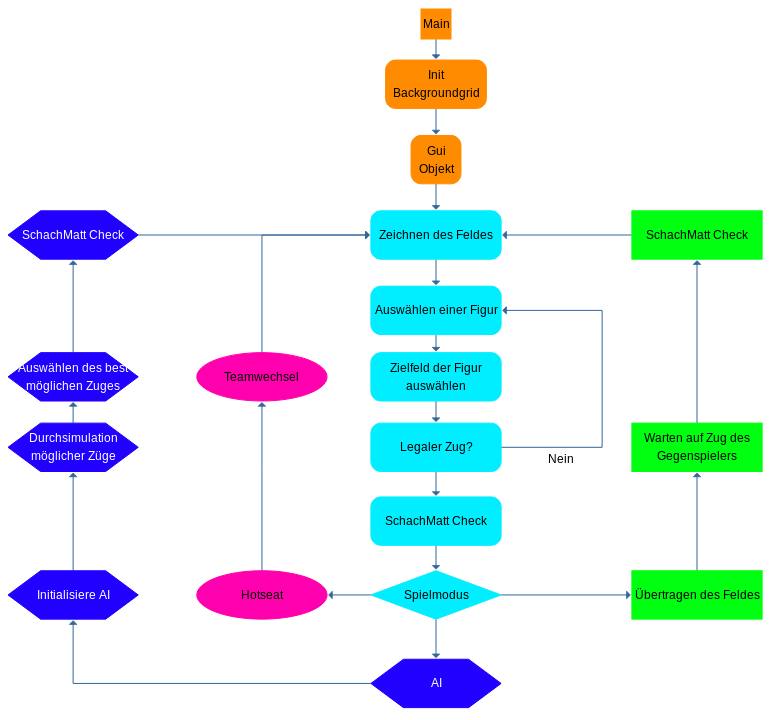
\includegraphics[width=14cm]{graphics/block.png}
  \caption{Das Blockschaltbild}
  \label{fig:block}
\end{figure}

\newpage
\subsection{Package- und Klassenübersicht}
\label{SUBSEC:PACKAGE}

Im Folgenden werden die groben Inhalte und Funktionen der Packages und Klassen zusammengefasst.\

\subsubsection{audio}

Dieses Package beinhaltet alle Klassen, die benötigt werden, um die Soundeffekte im Spiel abzuspielen. Zusätzlich sind die benötigten Audiofiles enthalten.\

\begin{itemize}
	\item{\textbf{AudioManager.java}: Diese Klasse managt die zwei Möglichkeiten, Audiodateien im Programm abzuspielen. Warum dies notwendig ist, wird in der entsprechenden Sektion erklärt. %TODO
Auch die Einstellungsvariablen für die Sounds (z.B. Lautstärke) werden hier gespeichert. }
	
	\item{\textbf{JavaFxAudio.java}: Mit dieser Klasse werden die Sounds für den JavaFX - Soundplayer geladen und abgespielt. }	
	
	\item{\textbf{NativeAudio.java}: Dies Klasse wurde nachträglich hinzugefügt und ermöglicht das Abspielen von Sounds auf Systemen, welche den JavaFX-Soundplayer nicht unterstützen, wie Ubuntu Version 14.1 und später.}
	
\end{itemize}

\subsubsection{backgroundmatrix}

In diesem Package sind Klassen beheimatet, die für die Spiellogik verantwortlich sind.

\begin{itemize}
	\item{\textbf{BackgroundGrid.java}: Dies ist eine ,,Basisklasse'' der Spiellogik. In ihr werden Schach- und Schachmattabfragen durchgeführt. Zusätzlich werden in ihr verschiedene spielrelevante Variablen gespeichert, beispielsweise das aktuell ziehende Team.}
	
	\item{\textbf{Move.java}: In dieser Klasse werden die erlaubten Zugmuster für jede einzelne Figur vermerkt und ausgewertet.  }

\end{itemize}
 
\subsubsection{game}

Die Klassen für die einzelnen Spielmodi werden in diesem Package abgelegt. 


\begin{itemize}

	\item{\textbf{AI.java}: Ist quasi Schnittstelle zwischen AILogic und dem restlichem Spiel. Sie wird als neuer Thread gestartet, um das restliche Spiel nicht zu beeinträchtigen. Ruft AILogic auf.}
	
	\item{\textbf{AILogic.java}: Hier ist der eigentliche KI-Algorithmus. Wertet alle möglichen Züge nach dem Bestmöglichen aus.}

	\item{\textbf{AIvsAI.java}: Diese Klasse reguliert den ,,geheimen Spielmodus'', in dem der Computer gegen sich selbst spielt. }
	
	\item{\textbf{LAN.java}: In dieser Klasse werden alle Variablen für den LAN-Spielmodus gespeichert. Zudem werden die Schnittstellen zur Netzwerkkommunikation bereitgestellt.}
	
	\item{\textbf{Local.java}: Diese Klasse beinhaltet die Variablen für den lokalen Modus. }

	\item{\textbf{MovePos.java}: Diese Klasse stellt eine Hilfsklasse dar. Sie wird benutzt, um die momentane, zukünftige, vergangene oder Spezialposition von Figuren zu bestimmen.}

\end{itemize}

\subsubsection{gui}

In diesem Package sind alle Klassen zusammengefasst, die etwas mit der GUI, also mit dem ,,Graphical User Interface'' zu tun haben. 

\begin{itemize}

	\item{\textbf{About.java}: Diese Klasse generiert ein Popup, welches Auskunft über die Entwickler und die Lizenz gibt. }
	
	\item{\textbf{BoardGui.java}: In dieser Klasse wird das Schachbrett gezeichnet. Außerdem werden hier Usereingaben mit der Maus verarbeitet und es werden graphische Effekte erzeugt. Auch wird in dieser Klasse ein Teil des Spielflusses, insbesondere das Senden und Empfangen des LAN-Modus, geregelt. }
	
	\item{\textbf{GUI.java}: Diese Klasse erweitert die FX - Applikationsklasse. Sie stellt alle graphischen Elemente dar und regelt deren Platzbedarf. Manche Funktionen, wie beispielsweise das Starten eines neuen Spiels oder das Laden eines Spielfeldes, sind hier enthalten }
	
	\item{\textbf{Help.java}: Die Helpklasse erzeugt ein Popup, in welchem die Spielanleitung angezeigt wird.}
	
	\item{\textbf{Menu.java}: Die Menüklasse erzeugt das Spielmenü. Alle Funktionen aus dem Menü werden hier ausgeführt oder zumindest aufgerufen. Konkret werden Spielmodi gewechselt, Felder gespeichert oder geladen, neue Spiele gestartet und es werden die Popups aufgerufen.}
	
	\item{\textbf{Popup.java}: Diese Klasse erzeugt ein Popup, in dem viele Spielelemente konfiguriert werden können. Genauer werden die Lautstärke, AI-Schwierigkeit, und weitere kleine Einstellungen angeboten. Zusätzlich werden Informationen zum Spiel angezeigt. }
	
	\item{\textbf{Tile.java}: Diese Klasse repräsentiert ein Feld auf dem Schachbrett und enthält dessen Informationen.}

\end{itemize}

\subsubsection{images}

Dieses Package enthält alle Bilddateien, die benötigt werden, um das Spielfeld darzustellen. 

\subsubsection{launchpad}

In diesem Package sind alle Klassen beinhaltet, welche den Launchpad-Support ermöglichen. 

\subsubsection{network}

Dieses Package beinhaltet alle Klassen, die benötigt werden, um den Netzwerkspielmodus zu ermöglichen.

\begin{itemize}
	\item{\textbf{Heartbeat.java}: Diese Klasse stellt sicher, dass der Verlust einer Netzwerkverbindung erkannt wird.}
	\item{\textbf{hostingJob.java}: Diese Klasse wird benötigt, um das Hosten eines Netzwerkspieles zu regeln. Genaueres dazu unter (\ref{SUBSUBSEC:CONHOST})} %TODO
	\item{\textbf{ReadingJob.java}: Diese Klasse ermöglicht es, Objekte vom Netzwerk zu empfangen. }
\end{itemize}

\subsubsection{saveload}

\begin{itemize}

	\item{\textbf{Load.java}: Diese Klasse enthält alle notwendigen Funktionen, um Spielstände zu laden. Außerdem werden alle Fehler, die beim Ladevorgang auftreten können, hier bearbeitet.  }
	
	\item{\textbf{Save.java}: Um Spielstände zu speichern, wird diese Klasse benötigt. Sie enthält alle notwendigen Funktionen dazu und bearbeitet Fehler, die beim Speichern auftreten können. }


\end{itemize}

\subsubsection{start}

Dieses Package enthält die Klasse ,,\textit{Main.java}'', welche nur dazu dient, das Spiel zu starten.

\newpage
\subsection{Initialisierung}
\label{SUBSEC:INIT}

\cmnt{Hier soll erklärt werden wie JavaChess initialisiert wird.}

Als Referenz bzw. Hilfe siehe \ref{SUBSUBSEC:BLOCKSCHALTBILD}.
Zuerst startet das Programm in der Main-Methode der Main-Klasse. Als Nächstes wird das Backgroundgrid-Objekt und das GUI-Objekt von der GUI-Klasse initialisiert. \\
Dieses Objekt ladet im Anschluss die BoardGui-Klasse, welche eine Abstraktion eines Canvas ist. In einem Canvas ist eine gewisse Art des Zeichnens möglich. Dadurch wird auch das Schachbrett gezeichnet und weiteres findet in dieser Klasse der ,,Spielfluss'' statt. \\ 
Im Default-Modus startet das Spiel im Hot-Seat Game-Mode, siehe \ref{SUBSEC:LOCAL_MODE}. Hier spielt der Spieler zuerst einen Zug, woraufhin kontrolliert wird, ob der Zug legal ist. Da das Spiel im Hot-Seat-Mode startet, wechselt der Spieler und das Schachbrett wird mit der Aufstellung nach Zug eins neu gezeichnet.

\subsection{Repräsentation der Figuren:}

Die Figuren werden über eine Zahlenmatrix repräsentiert. Dabei bekommt jede Figur eine individuelle Zahl zugeteilt. \\
Eine solche Zahl besteht aus drei Ziffern, z.B.: 102. Diese ist der zweite weiße Bauer, die erste Ziffer gibt dabei an, ob es Team Weiß (1) oder Schwarz (2) ist. Die zweite Ziffer gibt den Figurentyp an, also Bauer, Turm, etc. Die dritte Ziffer gibt an, die wievielte Figur es ist. \\
Diese Matrix ist in einem Objekt von der ,,Background-Matrix'' gespeichert. \\
Zu Beginn einer jeden Partie wird einmal die Startaufstellung im ,,Konstruktor'' der ,,Background-Matrix'' initialisiert:

	\begin{table}[H]
		\centering
		\begin{tabular}{| c | c | c | c | c | c | c | c |}
			\hline
			110 & 120 	& 	130 & 140 	& 150 	& 131 	& 121 	& 	111 \\ \hline
			101 & 102 	& 	103 & 	104 & 	105 & 	106 & 	107 & 	108 \\ \hline
			0	&	0	& 	0	&	0	&	0	&	0	&	0	&	0	\\ \hline
			0	&	0	& 	0	&	0	&	0	&	0	&	0	&	0 	\\ \hline
			0	&	0	& 	0	&	0	&	0	&	0	&	0	&	0 	\\ \hline
			0	&	0	& 	0	&	0	&	0	&	0	&	0	&	0 	\\ \hline
			201 &	202 &	203	&	204	&	205	&	206	&	207	&	208	\\ \hline
			210 & 	220	&	230	&	240	&	250	&	231	&	221	&	211 \\ 
			\hline	
		\end{tabular}
		\caption{Repräsentation der Figuren}
		\label{TABLE:REPRESENTATION-MEEPLES}
	\end{table}

\subsection{Zugmechanik und Local-Mode}
\label{SUBSEC:LOCAL_MODE}

Sobald das Spiel geladen und initialisiert ist, wird automatisch der Hot-Seat Spiel- modus ausgewählt. Beim Hot-Seat Modus spielt man auf einem Device nacheinander. Dieses eigentliche Spiel geschieht in einem Objekt der ,,BoardGui'' Klasse. Die BoardGui Klasse ist ein Canvas Objekt, also ein Objekt, auf dem man zum Beispiel zeichnen kann. Diese Funktion wird ausgenutzt, um das Spielfeld zu zeichnen. Wie dies genau geschieht wird in \ref{SUBSUBSEC:BOARDGUI}
erläutert.  \\
Nun ist der weiße Spieler an der Reihe. Welches Team an der Reihe ist, wird durch den Boolean ,,team'' bestimmt. Dieser Spielstand wird in einem Objekt der Backgroundgrid Klasse gespeichert. True bedeutet, dass der weiße Spieler am Zug ist, false, dass der schwarze am Zug ist. \\
Der Spieler kann nun die Figur anwählen, die er bewegen möchte, oder die linke Maustaste gedrückt halten und so die Figur via Drag \& Drop aufnehmen. In dieser Position werden alle möglichen Bewegungen des Spielsteins angezeigt. Hier ist zu erwähnen, dass potenzielle Angriffe in rot und mögliche Bewegungen in grün dargestellt werden.\\
Nun muss der Spieler nur noch das Feld, auf das er ziehen möchte, anklicken bzw. die Figur darüber absetzen. Der Move Algorithmus berechnet nun, ob dieser Zug auch möglich ist. Falls dieser Zug erlaubt ist, wird die Hintergrundmatrix, also das Spielfeld, entsprechend mit den neuen Positionen der Figuren, umgeschrieben. \\
Im Hot-Seat Modus wird jetzt das Team gewechselt und die GUI neu gezeichnet, damit die Änderungen in der Matrix sichtbar werden. 

\subsubsection{Die Move-Klasse - Funktion}
\label{SUBSUBSEC:MOVE}

Wie in \ref{SUBSEC:LOCAL_MODE} beschrieben, gibt es eine Abfrage, ob ein Zug erlaubt ist. Dafür gibt es aber mehrere Möglichkeiten:\\
Der erste Ansatz besteht darin, dass jede Figur ihren erlaubten Zug selber überprüft. Hierbei muss klar sein, dass wir für jede Figur ein eigenes Objekt des jeweiligen Klassentypes (z.B.: Bauer) angelegt haben. Für die Zugüberprüfung wird an die Figur die Position übergeben, wohin sie ziehen soll und das momentane Spielfeld, als 8x8 Matrix. Ein Boolean als Rückgabewert indiziert, ob dieser Zug legal ist. \\
Bevor eine solche Move-Abfrage aber überhaupt durchgeführt werden kann, muss diese auch aufgerufen werden und erkannt werden, welcher Spielstein ausgewählt wurde. Dies geschieht in einem Abschnitt der BoardGui-Klasse. \\
Der erste Ansatz ist somit nicht wirklich eine Klasse, sondern auf viele Klassen verteilt. Dies funktioniert ohne bekannte Bugs, dadurch wird der Code aber stellenweise sehr unübersichtlich. Weiteres verbraucht das Spiel teilweise mehr Ressourcen als unbedingt notwendig. Eine AI und eine Zugindikation mit diesem Ansatz zu schreiben ist, aber schlicht unvorstellbar. \\[2ex]
Der zweite Ansatz besteht darin, alle Zugabfragen in einer Klasse zu implementieren. Dazu wurde dem Objekt dieser Klasse die aktuellste Position und die Zielposition in Form von Koordinaten wie auch das Spielfeld übergeben. Geprüft wird wieder, ob der Spielzug erlaubt ist. Die Abfrage, welcher Spielstein ausgewählt wurde, geschieht über eine separate Klasse.\\ 
Vorteile ergeben sich aus der Übersicht. Die Nachteile sind aber nach wie vor der Ressourcenverbrauch, die Schwierigkeit eine Zugindikation zu programmieren und eine KI-Kompatibilität zu schaffen.\\[2ex]
Der dritte Ansatz beschäftigt sich mit der Vorschau der möglichen Züge. Man gibt dem Objekt der Move Klasse einfach alles, was bereits im zweiten Ansatz übergeben wurde. Nun wird aber ein Integer-2D-Array aus möglichen Zügen zurückgegeben. Dies funktioniert ohne Probleme. \\
Das Einzige, das als Problem deklariert werden kann, ist, dass dadurch das ,,DRY''-Prinzip (Don't repeat yourself)  verletzt wird. In der Move Klasse gibt es nun einmal die Abfrage, ob der Zug erlaubt ist und einmal die Abfrage, welche Züge möglich sind. Für die KI ist es von Vorteil, wenn sie alle möglichen Züge eines Spielsteines bekommt. Es sollte aber auch klar sein, welcher Spielstein zuvor auf dem Feld stand, was durch diese Methode nur indirekt möglich ist. \\[2ex]
Der vierte Ansatz nimmt sich allen diesen Problemen an, indem der dritte Ansatz ausgebaut wird und eine neue ,,MovePos''-Klasse eingeführt wird. Die Move-Klasse kann nun als eine Art Black-Box verstanden werden: Man sagt der Move Methode, welche Figur man ausgewählt hat und man erhält alle möglichen Züge als MovePos-ArrayList zurück. Der eigentliche Zug muss aber extern durchgeführt werden. \\
Das Objekt der Klasse MovePos beinhaltet die alte Position des Spielsteins, die neue Position, die ID des Spielsteins, die ID des Feldes, auf das gezogen wurde und für die Rochade bzw. den En-Passant noch zwei weitere Informationen zu den Feldern, wo und was darauf war. Die Klassen der Figuren werden nicht mehr benötigt. \\
Dadurch wird für die KI-Berechnung, für die Schachmatt-Methode, für die Zugüberprüfung und für das Anzeigen aller möglichen Züge die gleiche Basisstruktur der Zugberechnung verwendet. Der Unterschied besteht darin, dass die KI direkt die Zugberechnung aufruft, währenddessen die Zugüberprüfung und das Anzeigen der möglichen Züge indirekt, durch die GetMove-Methode, darauf zugreift.\\

\newpage
\subsubsection{Die Move-Klasse - Code}
\label{SUBSUBSEC:MOVECODE}

Die folgende Dokumentation erfolgt als Pseudo-Code. \\
Zuerst wird die GetMove-Methode beschrieben. Diese wird für die Spielerzüge verwendet. Sobald ein Spieler auf ein Feld klickt, bzw. bereits eines angeklickt hat und nun einen Zug tätigen will, wird diese Methode ausgeführt. \\

\lstset{language=Java}
\begin{lstlisting}
import...
...
public class Move{
	...
	public Move(){
		_bSelect = false;
		...
		das Standardmaessig keine Figur ausgewaeht wurde
		...
	}			
	...
	//Methode fuer Spielerzug bzw. zum anzeigen aller moeglichen Positionen
	public int[][] GetMove(Position und ID von Spielfigur, Objekt von Hintergrundmatrix){
		...
		iDif = Differenz zwischen zuvor ausgewaehlter und jetzt ausgewaehlter Figur/ ausgewaehltem Spielfeld
		
		if(Die Figrur darf bewegt werden){
			//ArrayList von der Klasse MovePos-moegliche Zuege
			ArrayList MoveList = Bekomme alle moeglichen Zuege der Figur (getMoveMeeple)
			for(Durch alle moeglichen Zuege){
				if(Die Figur darf auf das ausgewaehlte Feld ziehen){
					...
					Das Feld wird mit den neuen Positionen ueberschrieben
					Das ,,Feld'' wird in der BackgroundGrid Klasse als iBackground[][] gespeichert
					Der Zug wird als getaetigter Zug in die zuletzt-getaetigter-Zug ArrayList geschrieben
					...		
				}
				
			}
		} else {
			...
			
			...
			if(Position ist Figur){
				ArrayList MoveList = Bekomme alle moeglichen Zuege der Figur (getMoveMeeple)
				for(Durch alle moeglichen Zuege){
					if(Zug auf Leeres Feld){
						_MoveList.add(GezogenesFeld)
					}else{
						_HitList.add(GezogenesFeld)
					}
				}
			}
		}	
		return GeaendertesSpielfeld		
	}
	\end{lstlisting}
	Die getMoveMeeple-Methode gibt alle möglichen Spielzüge einer Figur zurück. Die Rückgabe erfolgt als eine MovePos-ArrayList. Ein Objekt der Klasse MovePos beinhaltet einen möglichen Zug einer Figur, z.B.: Bauer von A2 auf A3. \\
	Die getMoveMeeple-Methode unterscheidet zuerst nach der ausgewählten Figur, sprich Bauer, Turm, Läufer, Springer, Dame oder König. \\
	Je nach Figur wird überprüft, ob die figurspezifischen Züge möglich sind. Falls ein solcher Zug möglich ist, wird dieser in die ArrayList geschrieben, welche am Ende zurückgegeben wird.
	
	\lstset{language=Java}
	\begin{lstlisting}
	//Herzstueck der Move Klasse - gibt alle moeglichen Zuege zurueck
	public ArrayList getMoveMeeple(Spielfeld, Position von Spielfigur){
		new ArrayList MovePos...MP
		if(Bauer){
			//Zuege
			if(einfacher Zug moeglich){
				MovePos Zug...
				...
				MP.add(Zug) 
				...			
			}
			if(zweifacher Zug moeglich){
				MovePos Zug...
				....
				MP.add(Zug)
				...
			}
			//Schlaege
			if(weisses Team){
				if(Schlag diagonal nach links moeglich){
					MovePos Zug...
					....
					MP.add(Zug)
					...
				}
				if(Schlag diagonal nach rechts moeglich){
					MovePos Zug...
					....
					MP.add(Zug)
					...
				}
			} else {
				if(Schlag diagonal nach links moeglich){
					MovePos Zug...
					....
					MP.add(Zug)
					...
				}
				if(Schlag diagonal nach rechts moeglich){
					MovePos Zug...
					....
					MP.add(Zug)
					...
				}
			}
			//EnPassant
			if(min. 2. Zug){
				...
				letzerZug = getLastMove
				...
				if(wenn feindlicher Bauer danebensteht && ID letzer Zug == id Bauer daneben && Im letzen Zug 2 Felder bewegt worden sind){
					MovePos Zug...
					....
					MP.add(Zug)
					...
				}
			}	
		}else if(Turm){
			for(i=1 bis 7){
				if(Feld in X bzw. Y Richtung Ziehbar bzw. Figur schlagbar && keine Figur dazwischen) {
					MovePos Zug...
					....
					MP.add(Zug)
					...
				}
			}
		
		}else if(Springer){
			if(Feld auf eine von acht Arten ziehbar / schlagbar){
				MovePos Zug...
				....
				MP.add(Zug)
				...
			}
		}else if(Lauefer){
			for(i=1 bis 7){
				if(Feld in eine von vier Richtungen schlagbar/ziehbar){
					MovePos Zug...
					....
					MP.add(Zug)
					...
				}
			}
		}else if(Dame){
			for(i=1 bis 7){
				if(Feld in eine von vier Richtungen schlagbar/ziehbar){
					MovePos Zug...
					....
					MP.add(Zug)
					...
				}
				if(Feld in X bzw. Y Richtung Ziehbar bzw. Figur schlagbar && keine Figur dazwischen) {
					MovePos Zug...
					....
					MP.add(Zug)
					...
				}
			}
		
		}else if(Koenig){
			if(Standard Zuege moeglich){
				MovePos Zug...
				....
				MP.add(Zug)
				...
			}
			if(Feld 4 Felder links vom Koenig leer){
				if(Check Rochade Bedingungen-alle Felder dazwischen leer-kein Feld ist bedroht){
					MovePos Zug...
					....
					MP.add(Zug)
					...
					
				}
			}
			if(Feld 3 Felder rechts vom Koenig leer){
				if(Check Rochade Bedingungen-alle Felder dazwischen leer-kein Feld ist bedroht){
					MovePos Zug...
					....
					MP.add(Zug)
					...
				}
			}
		
		}
		
		return MP;
	}
	
	...
	Methode Bauerntausch - falls ein Bauer die entsprechende Position erreicht hat, wird auf diese Position eine Dame gesetzt
	...
	getSchach //ueberprueft ob Koenig im Schach ist (=vl. illegaler Zug)-via Schachmatt Methode
	getSchach2 //ueberprueft ob Koenig im Schach ist (Warnung an Spieler)-via Schachmatt Methode
	...
	getter und setter Methoden fuer Private Variablen
}
\end{lstlisting}
%\lstset{language=German}

\newpage
\subsection{Schach-, Schachmatt- und Patt-Abfrage}
\label{SUBSEC:checkmate}

\subsubsection{BackgroundGrid - Klasse}

Die Schachmatt-Abfrage befindet sich in der BackgroundGrid-Klasse. Diese Klasse beinhaltet alle wichtigen Variablen und dient intern quasi als Speicher. So wird in der BackgroundGrid-Klasse das momentan am Zug befindliche Team und die Zughistorie abgespeichert. \\
Diese Klasse implementiert auch ,,Serializeable'', womit ein Objekt dieser Klasse in der Speichern-Funktion in eine Datei geschrieben wird. \\

\subsubsection{Schachmatt - Übersicht}

Die Schachmatt-Abfrage teilt sich in drei Methoden innerhalb der Backgroundgrid Klasse auf:
\begin{itemize}
	\item{\nameref{SUBSUBSEC:check}}
	\item{\nameref{SUBSUBSEC:checkmate}}
	\item{\nameref{SUBSUBSEC:checkking}}
\end{itemize}



\subsubsection{Schach}
\label{SUBSUBSEC:check}

Die Schachmethode kann auf JEDE Figur angewendet werden und gibt TRUE zurück, wenn diese von einer anderen Figur angegriffen werden kann. Logisch gesehen gibt sie FALSE zurück, wenn die Figur nicht angegriffen werden kann. \\
Im Prinzip werden alle Figuren aufgerufen und überprüft, ob diese die ausgewählte Figur angreifen können. \\
\newpage
\textbf{Pseudo Code:}

\lstset{language=Java}
\begin{lstlisting}
private boolean Schach(Spielfeld, Lokation der Spielfigur auf die Schach angewendet werden soll){
	for(alle Figuren){
		if(Figur ist Bauer und kann Spielfigur angreifen){
			return true;		
		} else if(Figur ist Turm und kann Spielfigur angreifen){
			return true;
		} else if(Figur ist Springer und kann Spielfigur angreifen){
			return true;
		} else if(Figur ist Laeufer und kann Spielfigur angreifen){
			return true;
		} else if(Figur ist Dame und kann Spielfigur angreifen){
			return true;
		} else if(Figur ist Koenig und kann Spielfigur angreifen){
			return true;
		}
		
	}
	
	return false;	
}
\end{lstlisting}
%\lstset{language=German}

\subsubsection{Schachmatt}
\label{SUBSUBSEC:checkmate}

Die Schachmatt-Methode kann nur auf den König angewendet werden. Diese überprüft nacheinander alle Bedingungen, die erfüllt sein müssen, damit der König wirklich schachmatt ist. Anfangs wird überprüft, ob er dem Angreifer ausweichen kann bzw. schlagen kann. Falls dies nicht möglich ist, wird überprüft, ob der Angreifer selbst geschlagen werden kann. \\
Anschließend wird überprüft, ob es möglich ist, zwischen dem Angreifer und dem König mit irgendeiner Figur zu springen. \\
Pseudo-Code:

\lstset{language=Java}
\begin{lstlisting}
private boolean Schachmatt(Spielfeld, ID und Postion des Koenigs, Backgroundgrid Objekt){
	for(Positionen wo Koenig hinziehen kann){
		if(Position nicht bedroht){
			return false;
		}
	}
	
	if(Schach Methoden auf Angreifer anwenden == TRUE){
		return false;
	}
	
	for(alle moeglichen Zuege des Angreifers){
		for(alle Figuren des anderen Teams){
			for(alle Zuege der Figur)
				if(Zug moeglich && dadurch Koenig nicht mehr im Schach){
					return false;
				}
			}			
		}
	}
}
\end{lstlisting}
%\lstset{language=German}


\subsubsection{Schachking}
\label{SUBSUBSEC:checkking}

Die Schachking-Methode wird immer am Ende eines Zuges aufgerufen und überprüft, ob ein Team schachmatt ist. Falls dieses nicht schach, also der König im schach steht, oder schachmatt ist, wird nachgesehen, ob eine Patt-Situation vorherrscht. Dies geschieht in der Draw-Methode. \\
Falls ein Team schach ist, wird nachgesehen, ob dieses auch schachmatt ist. \\
Pseudo-Code:

\lstset{language=Java}
\begin{lstlisting}
public boolean Schacking(team,Spielfeld,auf welche Figur/Position die Abfrage gemacht werden soll, Schachmatt/Schach, simulierter Koenig){
	ID = ID des Koenigs
	
	Schach Abfrage auf ID
	
	if(wenn Schach nicht zutrifft und Schachmatt ausgefuehrt werden soll){
		Patt Situation soll ermittelt werden
	}
	if(wenn Schach zutrifft und Schachmatt ausgefuehrt werden soll){
		Schachmattabfrage
		if(Schachmatt trifft zu und weisses Team){
			weisses Team verliert
		}	
		if(Schachmatt trifft zu und schwarzes Team){
			schwarzes Team verliert
		}
	}
}
\end{lstlisting}
%\lstset{language=German}

\subsubsection{DRAW (Patt)}
\label{SUBSUBSEC:draw}

Die CalcDraw-Methode überprüft, ob ein Unentschieden entstanden ist. Welche Möglichkeiten es für ein Unentschieden gibt, findet man in den \nameref{SUBSEC:GAMERULES}. \\
Zuerst wird gezählt, wie viele Figuren das jeweilige Team noch hat. Wenn nur mehr der König übrig ist, wird überprüft, ob ein Patt vorherrscht. Es werden alle möglichen Züge des Königs durchsimuliert und falls kein gültiger dabei ist, herrscht ein Patt vor. \\
Weiters wird geprüft, ob sich ein Patt durch zu wenige Spielfiguren ergeben hat, falls dies ebenso nicht der Fall ist, werden noch Threefold-Repetition und die 50 Zug Regel überprüft. \\[2ex]
Die Methode CalcDraw ist eine Methode mit einem privaten Zugriffsmodifikator, womit nur Methoden innerhalb der BackgroundGrid Klasse darauf Zugriff haben. Die Methode ist eine Erweiterung der SchachKing-Methode, womit diese auch von dort aufgerufen wird. \\
Der Rückgabetyp der Methode ist ein boolean, welches true zurückgibt, wenn ein Unentschieden vorliegt und ansonsten false.

 \subsubsection{DRAW (Code)}
 \label{SUBSUBSEC:DRAW-CODE}

Folgende Dokumentation des Codes geschieht als Pseudo-Code:

\textbf{\lstset{language=Java}}
\begin{lstlisting}
private boolean CalcDraw(int iID, int[][] iBackground, int KingX, int KingY, boolean team, BackgroundGrid BGG ){
	
	int iSum1 = CountMeeplesForTeamWhite;
	int iSum2 = CountMeeplesForTeamBlack;
	
	if(Wenn der Koenig die letzte Spielfigur eines Teams ist){
		ArrayList-Typ-MovePos KingMoves = Bekomme alle moeglichen Zuege des Koenigs;
		for(Durch alle moeglichen Zuege durch gehen){ 
			...Mache den Zug auf der Hintergrundmatrix...
			if(Wenn bei einem Zug kein Schach vorherrscht){
				return false; //kein Draw
			}		
			..Mache den Zug rueckgaengig...
		}		
	} else if(Wenn zu wenige Spielfiguren uebrig sind, um ein Schachmatt noch zu erreichen){
		return true;		//Draw
	}
	
	if(Die Zugrunde ist >= 50){
		iMeeples = Alle nocht vorhandenen Figuren;
		
		for(bekomme Spielfelder der letzten 50 Zuege und gehe durch diese durch){
			iMeepleRef = Noch vorhandene Figuren zu Zug x
			if(iMeeples == iMeepleRef){
				count++; //Ein Zug wurde keine Figur geschlagen
			}
			
			if(Wenn die letzten 50 Zuege keine Figur geschlagen wurde und kein Bauer bewegt hat){
				return true;
			}
			if(Wenn sich in den letzten 50 Zuegen ein Bauer bewegt hat){
				return false;
			}
		}
		
	}else if(TurnRound >= 6){
		Bekomme alle Spielfelder 	
	
		if(Wenn eine Spielposition (ganzes Brett) drei Mal im Spiel vorkommt){
			Der Spieler kann ein Unentschieden proklamieren durch ,,threefold'' repetition
		}
	}
}
\end{lstlisting}



\newpage
\subsection{Die grafische Benutzeroberfläche}
Was wäre ein Spiel ohne grafische Benutzeroberfläche? Eine ansehnliche GUI (engl.: \textit{Graphical User Interface}) ist ein Kernbestandteil jeden Spieles. Um unsere Oberfläche vom Jahre 1998, dem Erscheinungsjahr von Swing, dem Toolkit das zuvor von uns verwendet und auch im Unterricht erlernt wurde, in die Gegenwart zu befördern, wird JavaFX verwendet. Mit JavaFX wurde ein modernes und Plattformunabhängiges Framework ausgewählt, um die grafische Oberfläche umzusetzen.

\subsubsection{JavaFX}
\label{SUBSUBSEC:JAVAFX}
JavaFX ist, wie schon erwähnt, das von uns verwendete Grafikframework für Java. Es stellt den designierten Nachfolger von Swing dar. Das Framework soll das Erstellen von plattformübergreifenden, multimedialen GUIs erleichtern und die Lücken, welche die veralteten Frameworks beinhalten, füllen.
Um JavaFX zu verstehen, wird nun die grundsätzliche Funktionsweise beschrieben.\\ [2ex]
Nach dem Start, der nicht mehr mit der ,,main-Methode'', sondern über eine Launch-Methode erfolgt, wird eine so genannte ,,Stage'' angezeigt. Vereinfacht kann man sagen, dass es sich dabei um das Fenster handelt, das angezeigt wird.\\
Auf der Stage werden überlicherweise eine oder auch mehrere ,,Scenes'' dargestellt. Eine Scene kann man sich wie einen Container vorstellen, der die grafischen Objekte des Programmes enthält. \\
Der Szenengraph besteht weiters aus Nodes (also Knoten). Es gibt ,,Parent-Nodes'', die weitere Nodes als Kinder enhalten können. Eine Node ohne weitere Kinder nennt man ,,Leaf''. Diese Leafs stellen die sichtbaren Elemente der GUI dar, also beispielsweise Buttons, Textfenster oder Ähnliches. Die Parent-Nodes sind sozusagen ,,innere Knoten'', die man sich als unsichtbare strukturelle Elemente vorstellen kann. Eine Applikation muss die Root-Node für eine Scene angeben. \\
Die Scene stellt das Bindeglied zwischen dem aus Nodes bestehenden Szenengraphen und dem vom Betriebssystem zur Verfügung gestellten Fenster dar. Um dies zu verstehen, nehmen wir beispielsweise an, wir wollen die Größe eines Fensters ändern. Sobald die Größe des Fensters verändert wurde, versucht die Scene, die Änderung an die Root-Node weiterzugeben. Dabei wird die Methode ,,isResizable'' der Root-Node aufgerufen, welche der Stage mitteilt, ob die Node auf Änderungen reagieren möchte. Ist dies der Fall, verändert die Scene die Größe der Nodes, ansonsten belässt die Scene die bestehenden Größen. Auf diese Weise vermittelt die Scene zwischen der Stage und den Nodes. 

\subsubsection{Das Darstellen des Schachfeldes}
\label{SUBSUBSEC:BOARDGUI}

Die erste Frage, die bei dem Erstellen der Gui aufgetreten ist, war wie das eigentliche Schachfeld seinen Weg auf den Bildschirm findet. 
Um diesen ursprünglichen Zweck zu erfüllen, wurde die Klasse ,,BoardGui.java'', die mittlerweile den Kern der grafischen Oberfläche, in dem das hauptsächliche Spielgeschehen stattfindet, eingeführt. \\
Die Klasse ist eine Erweiterung der Klasse ,,Canvas.java'', die mit dem JavaFX Framework Einzug in die Welt von Java gefunden hat. Das Canvas stellt eine Node dar (vgl.  \ref{SUBSUBSEC:JAVAFX}) und kann somit direkt auf einer Scene angezeigt werden.\\
Ein Canvas (dt. Leinwand) kann mit einer Zeichenfläche verglichen werden: Mithilfe eines sogenannten ,,GraphicsContext'', einer Klasse, die vom Canvas beinhaltet wird, können Methoden aufgerufen werden, die das Canvas in seiner Darstellung verändern. Somit ist es möglich, auf dem Canvas Linien, Formen, Farben und sogar Bilddateien ,,zu zeichnen''. \\
Da das Schachfeld im Spielverlauf sehr oft neu gezeichnet werden muss, wurde dieser Vorgang auf eine Methode ausgelagert. Diese nennt sich ,,redraw''. Was genau geschieht, wenn diese Methode aufgerufen wird, wird im Folgenden erläutert. \\[2ex]
Als erstes wird mithilfe des GraphicsContext auf der Größe des gesamten Canvas ein braunes Rechteck erstellt, um eine Grundierung für das Spielfeld zu erhalten. 
Im Anschluss wird die Methdoe ,,DrawGrid(Hintergrundmatrix)'' aufgerufen, die mithilfe der Hintergrundmatrix (vgl. Abb. \ref{TABLE:REPRESENTATION-MEEPLES}) das eigentliche Spielfeld mitsamt den Figuren darstellt.\\ 
Dort werden zuerst Skalierungsfaktoren erstellt, die es ermöglichen, die Längeneinheiten, die verwendet werden, um Formen zu generieren, unabhängig von der aktuellen Größe des Canvas, anzugeben. Diese Faktoren ergeben sich aus der simplen Teilung der aktuellen Canvasgröße durch den Faktor 100. Dadurch erhält man einen Wert, der einem Prozent der Canvasgröße entspricht. Nun ist es komfortabel möglich, die Positionen und Längen der anzuzeigenden Objekte am Bildschirm mithilfe dieses Skalierungswertes in einer prozentuellen Form anzugeben.\\
Im nächsten Schritt wird begonnen, ein Raster aus zuerst vertikalen und dann horizontalen schwarzen Linien zu ,,zeichnen''. Diese bestehen aus dünnen Rechtecken und sollen später die eigentlichen Schachfelder voneinander separieren und für eine saubere Trennung zwischen diesen sorgen.\\
In einer Schleife werden Werte nach oben gezählt, mit deren Hilfe die Linien in regelmäßigen Abständen dargestellt werden können. Die Abstände, in denen sich die Linien befinden, setzen sich zusammen aus dem Wert, den der Zählstand erreicht hat, multipliziert mit dem Skalierungsfaktor und der Summe aus der Breite einer Linie und der Breite eines späteren Schachfeldes.\\
Im Folgenden werden die bisherigen Schritte in Form von Pseudo-Code deutlich gemacht.\\
\lstset{language=java}
\begin{lstlisting}

		SkalierungX = Aktuelle Canvasbreite/100;
		SkalierungY = Aktuelle Canvashoehe/100;
		
		/* Zeichnen eines Rechtecks: 
		zeichneRechteck(PoistionX, PositionY, LaengeX, LaengeY);
		*/
	
	//vertikale Linien
		gc.setFill(Color.BLACK);
		for (Zaehlen von 1 bis 9) {
			 Abstand in X = (Zaehlstand * (Linienbreite in Prozent + Feldbreite in Prozent) * SkalierungX;
			 
			zeichneRechteck(Abstand in X, 0, Linienbreite * SkalierungX, aktuelle Canvashoehe);
		}

	//horizontale Linien		
		for (Zaehlen von 1 bis 9)) {
			 Abstand in Y = (Zaehlstand * (Linienbreite in Prozent + Feldbreite in Prozent) * SkalierungY;
			 
			zeichneRechteck(0, Abstand in Y, aktuelle Canvasbreite, Linienbreite * Skalierungsfaktor);
		}
		
\end{lstlisting}
Anmerkung: \textit{Im eigentlichen Code wird jeweils noch ein ,,Offset'' hinzugefügt, um Platz für die Beschriftung der Schachfelder zu lassen. Aus Verständlichkeitsgründen wurde hier jedoch auf die Erwähnung von diesem verzichtet.} \\[2ex]
Im Anschluss dazu werden die eigentlichen Schachfelder eingefärbt. Dies erfolgt in zwei verschachtelten for-Schleifen, wobei immer eine Zeile von links nach rechts eingefärbt wird, um dann in die nächste Zeile zu springen. Die Farbe der Felder wird nach dem Zählstand der zwei verschachteltetn Schleifen ausgewählt: Je nachdem, ob die Feldanzahl gerade oder ungerade ist, muss auch die passende Farbe verwendet werden. Die Positionierung der Felder geschieht mithilfe einer ähnlichen Formel wie zuvor für die Trennlinien. Diese setzt sich zusammen aus dem Zählstand der Schleifen, den Breiten der Felder und Linien und dem Skalierungsfaktor. Nach dem Determinieren der Farben und Längen wird ein Objekt der Klasse ,,Tile.java'' erstellt, dem für spätere Zwecke eine ID zugewiesen wird. Zusätzlich erhält es die Positionierungs- und Farbparameter, die benötigt werden, um ein Schachfeld darzustellen. Danach werden die Felder gezeichnet. 
Mithilfe des folgenden Pseudo-Codes sollen auch diese Schritte veranschaulicht werden.
\lstset{language=java}
\begin{lstlisting}

	
		for (y von 1 bis 8 zaehlen) {
			for (x von 1 bis 8 zaehlen) {
				if ((y == gerade) { // Even Odd
					if ((x == gerade) {
						farbe1();
					} else {
						farbe2();
					}
				} else {
					if ((x == gerade) {
						farbe2();
					} else {
						farbe1();
					}
				}
				
				PositionInX = Zahelstand in X * Linienbreite + Zaehlstand in X * Feldbreite;
				PositionInY = Zahelstand in Y * Linienbreite + Zaehlstand in Y * Feldbreite;
				Tile Feld = new Tile(PositionInX, PositionInY);
 				...  //eigenschafte des Feldes setzen (Farbe, ID etc.)
				ZeichneRechteck(PositionInX * SkalierungX, PositionInY * SkalierungY, Breite * SkalierungX, Hoehe * SkalierungY);

	
\end{lstlisting}
Anmerkung: \textit{Auch hier wurden die ,,Offsets'' für die Feldbeschriftungen der Einfachheit halber nicht erwähnt.}\\[2ex]
Die Darstellung der Figuren erfolgt über eine ähnliche Technik. Wieder handelt es sich um zwei verschachtelte Schleifen, die Zeile für Zeile abgearbeitet werden. Diesmal wird jedoch nicht unterschieden, ob die Zähler in den Schleifen gerade oder ungerade sind, sondern nach dem zugrundeliegenden Hintergrundraster unterschieden.\\
Die Figuren werden nicht über vordefinierte Formen dargestellt, sondern als Bilddateien geladen und mithilfe des GraphicsContext auf die Canvas gebracht. Die Position der Figuren unterscheidet sich bis auf einen Faktor, der die Figuren in die Mitte eines Feld setzt, nicht von den Positionen der Spielfelder. \\[2ex]
In folgendem Pseudo-Code wird auch dieser Teil des Codes veranschaulicht.
\lstset{language=java}
\begin{lstlisting}

		for (y von 1 bis 8 zaehlen) {
			for (x von 1 bis 8 zaehlen) {	
				PositionInX = PositionDesFeldesInX+Figurenkorrektur;
				PositionInY = PositionDesFeldesInX+Figurenkorrektur;
				Figurenzahl = Hintergrundraster bei Zeile x und Spalte y;
				//weisses team
				if (Figurenzahl < 110 && Figurenzahl >= 100) {
					ZeichneFigur(PositionInX, PositionInY, weisser Bauer);
				} else if (Figurenzahl >= 110 && Figurenzahl < 120) {
					ZeichneFigur(PositionInX, PositionInY, weisser Turm);
				} else if (Figurenzahl >= 120 && Figurenzahl < 130) { 
					ZeichneFigur(PositionInX, PositionInY, weisser Springer);
				} else if (Figurenzahl >= 130 && Figurenzahl < 140) { 
					ZeichneFigur(PositionInX, PositionInY, weisser Laeufer);
				} else if (Figurenzahl >= 140 && Figurenzahl < 150) { 
					ZeichneFigur(PositionInX, PositionInY, weisse Koenigin);
				} else if (Figurenzahl == 150) { // white king
					ZeichneFigur(PositionInX, PositionInY, weisser Koenig);
				}				
				 //schwarzes Team
				if (Figurenzahl < 210 && Figurenzahl >= 200) {
					ZeichneFigur(PositionInX, PositionInY, schwarzer Bauer);
				} else if (Figurenzahl >= 210 && Figurenzahl < 220) {
					ZeichneFigur(PositionInX, PositionInY, schwarzer Turm);
				} else if (Figurenzahl >= 220 && Figurenzahl < 230) {
					ZeichneFigur(PositionInX, PositionInY, schwarzer Springer);
				} else if (Figurenzahl >= 230 && Figurenzahl < 240) {
					ZeichneFigur(PositionInX, PositionInY, schwarzer Laeufer);
				} else if (Figurenzahl >= 240 && Figurenzahl < 250) { 
					ZeichneFigur(PositionInX, PositionInY, schwarze Koenigin);
				} else if (Figurenzahl == 250) { // black king
					ZeichneFigur(PositionInX, PositionInY, schwarzer Koenig);
				}
			}
		}

\end{lstlisting}
Um die Erstellung des Spielfeldes abzuschließen und eine Beschriftung für das Schachfeld einzubauen, werden zwei weitere Schleifen (diesmal allerdings nicht mehr verschachtelt) eingebaut. Anhand der Zählstände der Schleifen werden die passende Position der Beschriftung und der passende Buchstabe bzw. die passende Zahl bestimmt. Bevor der Text eingefügt wird, werden noch braune Flächen generiert, die genau in den zuvor freigelassenen Offset passen.
Anhand von folgendem Pseudo-Code wird auch dieser Vorgang veranschaulicht.
\lstset{language=java}
\begin{lstlisting}

	for (y von 0 bis 7 zaehlen) { 
			gc.fillRect(BreiteEinerLinie*SkalierungX, y*Offset*SkalierungY, Breite*SkalierungX, BreiteEinesFeldes*SkalierungY);
			bezeichnung=y+1;
			schreibeText(y);
		}

		for (x von 0 bis 7 zaelhen) {
			gc.fillRect(x*Offset*SkalierungX, BreiteEinerLinie*SkalierungY, BreiteEinesFeldes*SkalierungX,Breite*SkalierungY );

			switch (x) {
			case 0:
				s = "A";
				break;
			case 1:
				s = "B";
				break;
			
			...			
			
			case 7:
				s = "H";
				break;
			}
			schreibeText(s);
		}
	}

\end{lstlisting}
\newpage

\subsubsection{Klickbarkeit der Schachfelder}
\label{SUBSUBSECTION:CLICKABLE}
Um den dargestellten Feldern nun auch eine Funktion zu geben, muss man sie dazu bringen, auf Mauseingaben zu reagieren. \\
Unter JavaFX können die meisten Nodes mit so genannten ,,ActionListener'' bzw. ,,EventListener'' versehen werden. Dies sind Objekte, die ab ihrem Erstellungszeitpunkt auf einen bestimmten Typus von Ereignis warten. Die beschriebenen Ereignisse können Mauseingaben, aber auch Tastatureingaben oder die Veränderung einer bestimmten Variable sein. \\
Auch die Klasse ,,BoardGui.java'' kann mit solchen Event-Handlern versehen werden, da sie ja eine Tochterklasse der unter JavaFX standardmäßig enthaltenen Canvas-Klasse ist.\\
Um die Schachfiguren zu bewegen, wurde die Methode ,,setOnMouseReleased'' der BoardGui-Klasse verwendet. Diese Methode ist ein EventListener, der seinen Code ausführt, sobald ein Mausklick aufhört.
In diesem Listener wird nun jener Code ausgeführt, der die korrekte Aktion für den gerade aktiven Spielmodus ausführt. \\
In folgendem Pseudo-Code wird dies deutlich gemacht.

\lstset{language=java}
\begin{lstlisting}

for(jedes Feld){

	if(Feld ageklickt && Feld mit Figur besetzt){
		Figur angewaehlt;
	}else if(Feld angeklickt && Feld nicht mit Figurbesetzt && Figur angewaehlt){
			zugabfrage();
			if(Zug ist gueltig){
				if(Spielmodus ist lokal){
				... 	//Lokaler Modus
				}
				if(Spielmodus ist LAN){
				...		//LAN-Modus
				}
				if(Spielmodus ist AI){
				...		//AI-Modus
				}
			}	
	}
}

\end{lstlisting}
\subsubsection{Drag and Drop}
\label{SUBSUBSECTION:DRAGANDDROP}
Um eine alternative Möglichkeit zu bieten, die Figuren zu bewegen, wurde implementiert, Züge auch mittels Ziehen und Loslassen der Figuren durchführen zu können.\\
Dafür wurden zwei weitere Event-Listener benötigt: ,,setOnMouseDragged'' und \\ ,,setOnMousePressed''. Das Anwählen einer Figur wurde von der zuvor benutzten Methode ,,setOnMouseReleased'' in die neue Listener-Methode ,,setOnMousePressed'' verschoben. Diese führt ihren Code aus sobald ein Mausklick beginnt und nicht sobald er aufhört. Dies ist notwendig, da bei einem ,,Drag'', also beim Ziehen einer Figur, die Maus gedrückt gehalten werden muss.\\
Die Methode ,,setOnMouseDragged'' ruft immer, sobald eine Figur gezogen wird, die Redraw-Methode, also die Methode zum Zeichnen des Feldes, auf, wobei die Figurenposition der gezogenen Figur nun einfach auf die Position des Mauszeigers gesetzt wird.\\
Wenn das Ziehen einer Figur beendet ist, wird wieder der Code in der Methode ,,setOnMouseReleased'' ausgeführt (vgl. \ref{SUBSUBSECTION:CLICKABLE}).


\subsubsection{Hervorheben bestimmter Felder}
\label{SUBSUBSECTION:TILEHIGHLIGHT}
Um auch Schachanfängern ein gutes Spielerlebnis zu ermöglichen, wurde die Funktion eingebaut, Felder hervorzuheben, auf die eine Figur ziehen kann.\\
Es gibt drei verschiedene Fälle, in denen Felder speziell markiert werden: 
\begin{itemize}

\item{Wenn auf eine Figur geklickt wird, werden alle leeren Felder, auf die die Figur ziehen kann, mithilfe einer Methode blau umrandet. Dafür wird für jedes leere Feld ermittelt, ob die Figur darauf ziehen darf. Ist dies der Fall, so wird die Markierung durchgeführt. }

\item{Ähnlich dem Markierungsvorgang für leere Felder werden schon besetzte Felder auch überprüft. Ist ein Zug möglich, darf die Figur auf dem Feld also geschlagen werden, so wird das entsprechende Feld, mithilfe einer eigenen Methode, rot umrandet.}

\item{Wenn ein Zug stattgefunden hat, wird das Feld, auf dem die Figur zuvor gestanden ist und jenes, auf dem die Figur nach dem Zug steht, grün eingefärbt. Dazu werden die betreffenden Felder nach dem Zug gespeichert. Das Einfärben geschieht dann direkt in der redraw-Methode, die um diese Funktion erweitert wurde. }


\end{itemize}

\subsubsection{Startup-Bildschirm und Informationsbildschirm}
\label{SUBSUBSEC:BLURRYMENU}
Um beim Starten des Programmes oder beim Warten auf eine Verbindung im LAN-Modus einen ansprechenden Informationsbildschirm darzustellen, wurden mehrere Methoden implementiert, die zwar unterschiedliche Schaltflächen anzeigen, jedoch im Kern gleich aufgebaut sind. Im Folgenden wird die grundsätzliche Erstellung dieser Informationsbildschirme erläutert\\
\begin{figure}[H]
  \centering
   	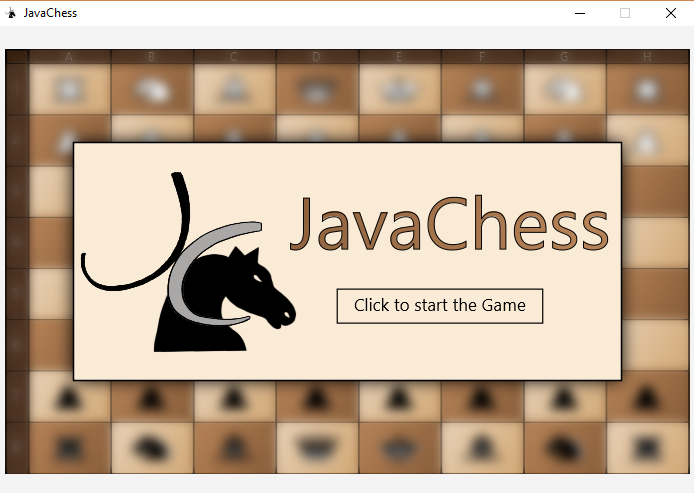
\includegraphics[width=14cm]{graphics/Startup.png}
  \caption{Informationsbildschirm beim Starten des Spiels}
  \label{fig:Startup}
\end{figure}

Als erstes wird die Klickbarkeit der Schachfelder mittels einer speziellen Deaktivierungsvariable entfernt. Im Anschluss wird ein Objekt der Klasse ,,BoxBlur'' erstellt. Dies ist ein graphischer Effekt, der standardmäßig mit JavaFx ausgeliefert wird. Man kann ihn vergleichen mit einer Art Filter, den man über graphische Objekte legen kann. Alles hinter diesem Filter erscheint dann verschwommen. \\
Mithilfe des GraphicsContext wird dieser Effekt dann auf unsere ,,BoardGui'' angewand. 
Im Anschluss wird ein braunes Rechteck generiert, das in die Mitte des Bildschirms gezeichnet wird. Auf diesem Rechteck wird später der Text des jeweiligen Informationsbildschirmes angezeigt. Um dieses Rechteck in den Vordergrund zu heben, wird ihm der Effekt ,,dropShadow'' hinzugefügt. Dies ist auch ein mit JavaFX mitgelieferter Effekt, der bewirkt, dass das dargestellte Objekt einen dezenten Schatten wirft.
Der dargestellte Text wird je nach Situation ausgewählt. Beim Starten des Programmes wird das Logo und der Titel angezeigt, im LAN-Spielmodus die entsprechenden Informationen (vgl. \ref{SUBSUBSEC:CONHOST}) angezeigt. \\
Zum Schluss wird noch ein ,,Event-Handler'' hinzugefügt, der auf Mausklicks reagiert. Je nach Situation bewirkt dieser Klick entweder nur ein Verschwinden des Informationsbildschirmes, oder es werden zusätzliche Befehle ausgeführt (vgl. \ref{SUBSUBSEC:CONHOST}). \\




\subsubsection{Die Menüleiste}
Um den Spielmodus zu ändern, das Schachfeld abspeichern zu können, oder weitere Optionen und Hilfefenster aufrufen zu können, soll am oberen Rand des Bildschirmes eines Menüleiste angezeigt werden. \\
Diese Menüleiste wird mithilfe der in JavaFx enthaltenen ,,MenuBar'' - Klasse realisiert. Diese stellt eine weitere Node dar, die speziell dafür gedacht ist, weitere Nodes in Form von Menüpunkten zu beinhalten und darzustellen.  Die von uns verwendete Klasse ,,Menu'' erbt von dieser Klasse. Im Folgenden wird beschrieben, wie die ,,Menu''-Klasse arbeitet. \\
Als erstes werden alle benötigten Untermenüs, in Form von den JavaFx bereitgestellten Untermenüs, erstellt. Im Gesamten werden vier dieser Menüs benötigt:
\begin{itemize}

	\item{\textbf{Game}: Dieses Menü beinhaltet alle Menüpunkte, die verwendet werden, um ein neues Spiel zu starten oder Spielstände zu laden und zu speichern.}
	
	\item{\textbf{Gamemodes}: In diesem Menü werden die verschiedenen Spielmodi ausgewählt. Zudem wird, wenn der LAN-Modus aktiv ist, eine Option angezeigt, um die Verbindung zu trennen.  
	}
	\item{\textbf{Other}: Weitere Informationen und die Option, ein Patt auszulösen, werden in diesem Menü untergebracht.}
	\item{\textbf{Help}: In diesem Menü können Informationen zum Spiel und die Hilfeseite aufgerufen werden. }
\end{itemize}
Dem jeweiligen Untermenü werden dann die entsprechenden Menüpunkte hinzugefügt. Auf jeden dieser Menüpunkte wird ein ,,EventListener'' aufgesetzt, der den richtigen Code beim Auswählen eines Menüpunktes ausführt. Die genaue Funktionalität der einzelnen Menüpunkte wird unter anderem in \ref{SUBSUBSEC:OPTIONS} beschrieben. 

\subsubsection{Die GUI - Klasse}
In der GUI-Klasse werden die Nodes zusammengeführt. Diese Klasse erweitert die ,,Applikation''-Klasse, also jene Klasse, die als Hauptklasse einer JavaFX Applikation angesehen werden kann. Sie wird beim Starten des Programmes initialisiert. In ihr werden die BoardGui-Klasse, die benötigt wird, um das Spielfeld zu zeichnen, und die Menu-Klasse, welche die Menüleiste mit allen ihren Untermenüs darstellt, initialisiert. Im Anschluss wird ein Objekt der Klasse ,,BorderPane'' erstellt. Dies ist auch eine Node, welche die Funktion hat, das Layout anderer Nodes auf dem Bildschirm zu regeln. Im Anschluss werden die Nodes ,,BoardGui'' und ,,Menu'' zu dieser BorderPane hinzugefügt. Diese BorderPane wird nun zu einer neu erstellten Scene hinzugefügt, welche wiederum zu der neu erstellten Stage hinzugefügt wird. Diese Stage wird dann am Bildschirm angezeigt. 
Zuletzt wird noch der Startupbildschirm (vgl. \ref{SUBSUBSEC:BLURRYMENU}) angezeigt (vgl. Abb. \ref{fig:Startup}).

\subsubsection{Informations- und Optionspopups}
\label{SUBSUBSEC:OPTIONS}
Um zusätzliche, nicht spielrelevante Informationen anzuzeigen, wurden die drei Folgenden Klassen erstellt: 
\begin{itemize}
\item{Popup.java}
\item{Help.java}
\item{About.java}
\end{itemize}
Die Klassen ,,About'' und ,,Help'' ähneln sich strukturell sehr. Das liegt daran, dass beide Klassen nur dazu da sind, Informationen anzuzeigen. Um diese Popups anzuzeigen, werden jeweils in der Klasse eine neue Stage und eine neue Scene erstellt, die bei Bedarf angezeigt werden können. \\
In der ,,About''-Klasse werden Informationen in Form von Labels, also Textflächen, bezüglich der Entwickler und der Lizenz des Programmes angegeben. Auch das Schachlogo wird angezeigt. Diese Nodes werden zur neu erstellten Scene hinzugefügt. Die Positionierung der Nodes erfolgte nicht skalierbar, also in absoluten Positionen.\\
In der ,,Help''-Klasse werden die anzuzeigenden Objekte prinzipiell gleich erstellt wie in der ,,About'' - Klasse. Da die Spielanleitung, die diese Klasse beinhaltet, allerdings relativ umfangreich ist, wurde der Text zu einer ,,ScrollPane'' hinzugefügt. Dies ist eine Node, die sich der Länge des Textes anpasst, der ihr übergeben wird. Wenn der Text über die Größe der ScrollPane hinausgeht, wird ein Scrollbalken angezeigt, mit dem durch den Text gescrollt werden kann. \\
In der ,,Popup''-Klasse werden zusätzliche Optionen zum Spiel bereitgestellt. Diese Optionen werden mithilfe von ,,Slidern'', ,,Buttons'' und ,,Checkboxen'', welche alle Kontrollelemente aus der JavaFX-Bibliothek darstellen, und auch zu einer neuen Scene und Stage hinzugefügt werden, verändert. 
Mithilfe von Listenern kann auch hier wieder ein spezieller Code beim Betätigen eines solchen Objektes ausgeführt werden.\\
Zusätzlich werden in dieser Klasse Informationen über das aktuelle Spiel, genauer die Rundenanzahl und das aktuell ziehende Team, mithilfe von Labels angezeigt. \\
Da alle drei Klassen eine neue Stage eröffnen, können sie parallel zum Spielfenster neue Fenster anzeigen. Dies muss auch nicht manuell auf neue Threads ausgelagert werden, da die JavaFX-Applikation diesen Vorgang automatisch beim Öffnen einer neuen Stage vornimmt. 
\begin{figure}[H]
  \centering
   	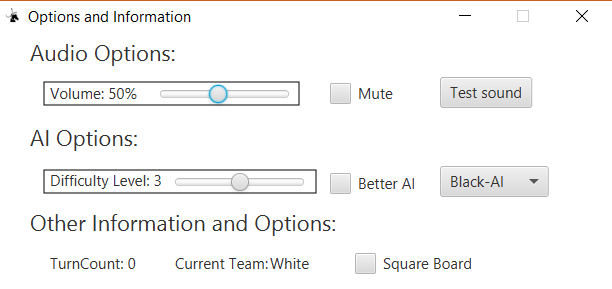
\includegraphics[width=14cm]{graphics/Menu.png}
  \caption{Optionspopup }
  \label{fig:options}
\end{figure}

\newpage
\subsection{Sounds}
Um dem Spieler eine bessere Erfahrung zu bieten, wurde die Entscheidung getroffen, Soundeffekte in das Spiel einzubinden. Die Entscheidung, das durch JavaFX bereitgestellte Sound - Framework zu verwenden, war naheliegend.

\subsubsection{Der JavaFX - Soundplayer}
Der Soundplayer sollte als eigene Klasse ausgeführt werden. Um ein einfaches Implementieren der Effekte zu ermöglichen, sollten die Sounds über eine spezielle Methode ausgewählt und abgespielt werden. \\
Als erstes werden die Audiodateien in das Programm geladen. Danach wird für jeden Sound  mithilfe dieser Dateien ein Objekt der Klasse ,,Media'' erstellt. Dies ist eine von JavaFX mitgelieferte Klasse und repräsentiert den Soundeffekt im Programm. Um die Effekte in der Lautstärke verändern zu können, oder sie ganz auszuschalten, werden zwei Variablen eingebaut. Diese können zur Laufzeit in den Optionen (vgl. \ref{SUBSUBSEC:OPTIONS}) verändert werden.\\
Um die Sounds später im Progamm abspielen zu können, wird die zuvor genannte Methode vorbereitet. Der Methode wird beim Aufrufen ein String mitgegeben, mit dem ausgewählt werden kann, welcher Sound abgespielt wird.\\
Zuerst wird in dieser Methode überprüft, ob der Sound ausgeschaltet ist. Im Anschluss wird anhand des Strings ausgewertet, welcher Effekt abgespielt werden soll. Nach der Auswertung wird ein Objekt der Klasse ,,MediaPlayer'' erstellt, welches es ermöglicht, die zuvor erstellten ,,Media'' - Objekte abzuspielen. Ihm wird das entsprechende ,,Media'' - Objekt mitgegeben. Danach wird die Lautstärke des ,,MediaPlayer'' - Objektes entsprechend der Variable gesetzt und der Sound wird abgespielt. \\
Der folgende Pseudo-Code veranschaulicht den beschriebenen Vorgang.

\lstset{language=java}
\begin{lstlisting}

//Constructor
	public JavaFxAudio() {
		Effekt1 = new Media(Soundfile1);
		Effekt2 = new Media(Soundfile2);
		...
		Effekt3 = new Media(Soundfile3);
	}
	
//Methode zum Abspielen der Sounds
public void playSound(Auswahlt) {
		if (Sound ist nicht Ausgeschaltet) {
			switch (Auswahl) {
				case "move":
					Player = new MediaPlayer(Effekt1);
					break;
				case "menu":
					Player = new MediaPlayer(Effekt1);
					break;
				case "startup":
					Player = new MediaPlayer(Effekt1);
					break;
			//Wenn kein Effekt ausgewaehlt wird
				default:
					break;
			}
			Player.setzeLautsaerke(Lautstaerke);
			Player.abspielen();
		}
	}
\end{lstlisting}

\subsubsection{Der alternative  Soundplayer}
\label{SUBSUBSEC:SOUNDBUG}

Nach dem Veranstalten interner Tests wurde festgestellt, das unter manchen Linux-Betriebssystemen die Initialisierung des Soundplayers fehlschlägt.\\
Nach umfangreichen Recherchen wurde das Problem festgestellt: Der JavaFX-Soundplayer verwendet Bibliotheken, die seit Ubuntu 14.0 nicht mehr unterstützt werden. Ohne diese Bibliotheken ist ein Abspielen des Sounds nicht möglich. \\Um das Problem zu umgehen wurde entschieden, einen Soundplayer zu entwickeln, der ohne die JavaFX - Bibliotheken auskommt. Dieser verwendet das Standard - Audioframework unter Java.  Das Konzept dieser Klasse ähnelt dem des ursprünglichen Soundplayers und wird deshalb nicht näher erläutert. Für Details ist der beiligende Code zu Rate zu ziehen. \\
Der Nachteil, den der native Soundplayer bietet ist, dass er weniger optimiert, ist und im Vergleich zum ursprünglichen Soundplayer wesentlich mehr RAM verbraucht. Um eine optimale Nutzung zu gewährleisten wurde eine ,,Audiomanager'' - Klasse eingebaut, die beim Start des Spiels versucht, den ,,FX - Soundplayer'' zu initialisieren. Im Falle, dass dies fehlschlägt, wird stattdessen der alternative Soundplayer eingesetzt. 

\newpage
\subsection{LAN-Mode}

Der LAN-Modus ist jener Spielmodus, mit dem die Spieler auch auf getrennten Computern miteinander spielen können. Dabei müssen sie sich in einem LAN, also im Local Area Network, befinden. Um zu verstehen, wie der LAN-Modus arbeitet, wird eine kurze Einführung in die Netzwerkprogrammierung unter Java gegeben. 

\subsubsection{Netzwerkprogrammierung unter Java}

Um unter Java eine Verbindung zwischen zwei Computern herzustellen werden so genannte ,,Sockets'' verwendet. Ein Socket ist ein Objekt, das die Netzwerkverbindung zwischen zwei Maschinen repräsentiert.\\
Unterschieden wird zwischen den Sockets der Clients, also jenen Teilnehmern, die eine Verbindung aufbauen wollen, und den Sockets der Server, also den Teilnehmern, die auf eine eingehende Verbindung warten.\\
Ein Objekt der Klasse Socket repräsentiert die Verbindung einens Clients, ein Objekt der Klasse ServerSocket die eines Servers.\\
Der große Unterschied zwischen den beiden Klassen ist, dass mit dem Serversocket keine Daten gesendet oder empfangen werden. Er ist einfach nur dazu da, auf  Verbindungen zu warten und diese anzunehmen. Sobald eine gültige Verbindung vorliegt, gibt der Serversocket ein Objekt der Klasse Socket zurück, über das der Server dann mit dem Client kommunizieren kann.\\[2ex]
Ein Problem an diesem System ist, dass der Serversocket während seiner Wartezeit den weiteren Ablauf des Programmes blockiert. Es kann also nicht weiter bedient oder gar beendet werden. Die Lösung dafür ist jedoch denkbar simpel: Der Serversocket wird während seiner Wartezeit auf einen anderen Thread, also einen Ausführungsstrang, ausgelagert. Dies erlaubt dem Programm, weiter auf Benutzereingaben zu antworten.\\[3ex]
Um nun auch Daten senden zu können, muss eine Kette aus ,,Streams'' erstellt werden. Streams sind Objekte, mit deren Hilfe Daten in ein Javaprogramm eingelesen oder geschrieben werden können. 
Um Objekte senden und empfangen zu können, werden Object-Input-, beziehungsweise Object-Output-Stereams verwendet. Dies sind Streams zur ,,Vorverarbeitung'', welche die Daten für einen ,,lowlevel-Stream'' vorbereiten. Der lowlevel-Stream kümmert sich dann um das schlussendliche Versenden der Daten. \\[2ex]
Wenn man nun Objekte mithilfe der Sockets versenden will, so erstellt man einen Object-Stream, welchem man den lowlevel-Stream des entsprechenden Sockets als Argument mitgibt. Diesen erhält man von einer Funktion des Sockets. War der Vorgang erfolgreich können nun ganz bequem mittels Funktion des entsprechenden Streams Daten gesendet und empfangen werden.

\subsubsection{Netzwerkprogrammierung in JavaChess}
\label{SUBSUBSEC:NETWORKJC}

In JavaChess gibt es einen Host und einen Client. Diese unterscheiden sich nur beim Verbindungsvorgang. Der Host wartet auf eine eingehende Verbindung, der Client baut aktiv eine Verbindung auf. Nach dem Aufbauen einer Verbindung wird der Serversocket vom Host zu einem ,,normalen'' Socket umgewandelt. Ab diesem Zeitpunkt befinden sich die beiden Teilnehmer im Spielfluss und führen den selben Code aus. Das bedeutet, dass sowohl der Code für den Host als auch der Code für den Client, bis auf die Verbindungsvorgänge, absolut identisch sind. 


\begin{figure}[H]
  \centering
   	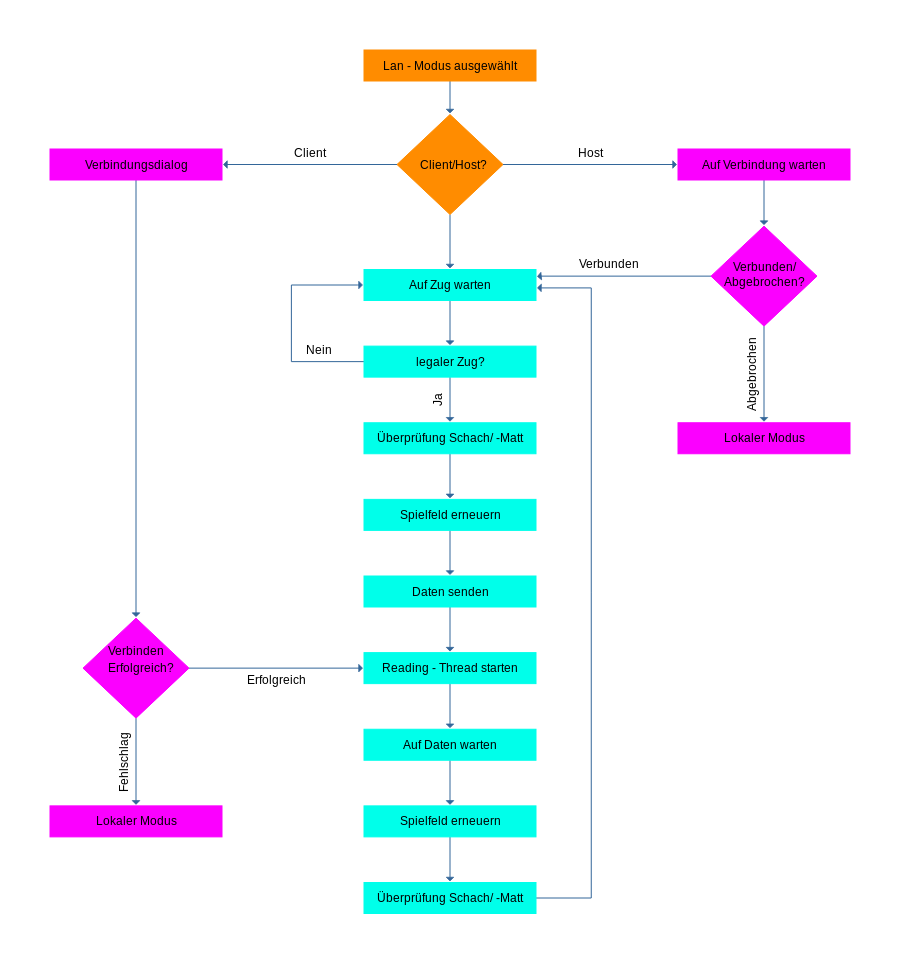
\includegraphics[width=16cm]{graphics/SpielflussLAN.png}
  \caption{Spielzyklus im LAN-Modus}
  \label{fig:lan}
\end{figure}


\subsubsection{Verbindungsvorgang des Clients}
\label{SUBSUBSEC:CONCLI}

Um mit dem Client eine Verbindung aufzubauen, muss in der Menüleiste der entsprechende Punkt angewählt werden. Es öffnet sich ein Dialogfenster. Wird in diesem Dialogfenster der Punkt ,,Join'' angewählt, beginnt der Verbindungsvorgang. \\[2ex]
Ein neues Dialogfenster wird angezeigt. Der Benutzer muss hier seine IP-Adresse eingeben. 
Ist die eingegebene Adresse korrekt, so wird der Socket der LAN-Klasse mit dieser IP-Adresse und einem fest vorgegebenen Port initialisiert. 
Ist auch dies erfolgreich, so wird das Team des Clients auf Schwarz gesetzt, die Streams zur Kommunikation erstellt und es werden ein Reader Thread und ein Heartbeat Thread gestartet.\\[2ex]

Folgender Pseudo-Code zeigt den Verbindungsvorgang: \\
\lstset{language=Java}
\begin{lstlisting}

if(join ausgewaehlt){				

					wechsleSpielmodus(Lan);				
					neuerDialog();
					...							//graphisches Design des Popups
					Optional<String> ipResult = ipDialogoue.showAndWait();
					if (IP Adresse eingegeben){										
						try {
								joinAdress = eingegebene Adresse();
								SocketErstellen();
								//Streams erstellen und Teams setzen	
								StreamsErstellen()
								Verbindungsstatus(Verbunden);
								Team(Schwarz);			
								//Zugverzoegerung um einen Zug		
								Zugverzoegerung(true);
								SchachfelderKlickbar(false);
								Thread rt = new Readinthread();  		
								rt.start();
								Thread th = new HeartbeatThreadThread(Heartbeat);
								th.start();
								//Menuepunke entfernen und hinzufuegen
								menuFile.getItems().removeAll(Speichern und Laden);
								menuGame.getItems().removeAll(Spielmodi);		
								menuGame.getItems().addAll(disconnect);	
								Gui.getBoardGui().DrawGrid(Hintergrundmatrix);		
								Gui.getBoardGui().redraw();
							}

						} catch (UnknownHostException) {
							...
							spielerBenachrichtigen();
							wechsleSpielmodus(Lan);		
							
						} catch (IOException e) {
							...
							spielerBenachrichtigen();
							wechsleSpielmodus(Lan);		
						} catch (ClassNotFoundException e) {
							spielerBenachrichtigen();
							wechsleSpielmodus(Lan);		
						}
\end{lstlisting}

\subsubsection{Verbindungsvorgang des Hosts}
\label{SUBSUBSEC:CONHOST}

Um ein Spiel zu hosten wird im Auswahldialog der entsprechende Punkt angewählt. 
Im Hintergund wird ein neues Spielfeld erstellt, der Spielmodus gewechselt, und es wird der ,,Hosting Thread'' gestartet.
Im Vordergrund wird eine Informationsfläche (vgl. \ref{SUBSUBSEC:BLURRYMENU}) gezeichnet. In diesem hat der Host die Option, den Wartevorgang abzubrechen und wieder in den lokalen Modus zurückzukehren. \\
Der folgende Pseudo-Code zeigt, was bei dem Abbruchvorgang passiert: 
\lstset{language=java}
\begin{lstlisting}

if(Verbindungsvorgang abgebrochen){

					SchachfelderKlickbar= true; 
					//widerherstellen der Menues
					menues ruecksetzen();		
						
					try{	
						HeartbeatThreadStoppen();
						HostingThreadStoppen();}
					} catch(Exception e){
						...			 //Fehlerbehandlung
					}
						in lokalen Modus wechseln();
						DrawGrid(_BGG);
					}
				}

\end{lstlisting}

Während die Schaltfläche für den Abbruch zu sehen ist, wird im Hintergrund der Hosting-Thread ausgeführt. Dieser erstellt den Serversocket, startet den Heartbeat-Thread (  (vgl. \ref{SUBSUBSEC:HEARTBEAT}) und wartet auf eine Verbindung. \\[2ex]
Ist der Verbindungsvorgang erfolgreich, so erzeugt der Thread den Socket der LAN - Klasse, der zum Spielen notwendig ist. Er erzeugt die Streams um die Kommunikation zu ermöglichen und setzt den Verbindungsstatus auf ,,verbunden''. \\
Anschließend muss noch die Schaltfläche zum Beenden des Wartevorganges verschwinden. Unter JavaFX kann die grafische Oberfläche allerdings nur von dem Hauptthread aus verändert werden.\\ 
Um dieses Problem zu umgehen, wird ein Objekt der Klasse Robot erstellt. Mit diesem ist es möglich, den Mauszeiger auf die Schaltfläche zu führen und einen Klick auszulösen. 
Dieser Klick wird im Hauptthread erkannt und das Feld wird neu gezeichnet. \\
Der folgende Pseudo-Code zeigt die Geschehnisse im Hosting-Thread:\\
\lstset{language=java}
\begin{lstlisting}

try {
				
				HeaertbeatThread= new Thread(Heartbeat);
				TeamSetzen(Weiss);
				//warten auf eingehende Verbindung
				tempsock = VerbindungDesServersockets();
				bgg.getLan().Streams erstellen();	//erstellen der Streams
				bgg.getLan().setIsConnectet(true);
				
				//Ruecksetzen des Menues
				Point b = Position der Maus
				int xOrig, yOrig = Urspruengliche Mausposition
		      
		            try {
		                Robot r = new Robot();
		                r.mouseMove(Position des Mauszeigers);
		                r.mousecklick(linke maustaste)
		                //mauszeiger an die originale Position bewegen
		                r.mouseMove(xOrig, yOrig);
		            } catch (Exception e) {
		                ...  	//Problembehandlung
		            }
			} catch (Exception e) {
				...	//Problembehandlung
			}		
		}

\end{lstlisting}

\subsubsection{Spielfluss im LAN-Modus}

Bis auf den Verbindungsvorgang unterscheiden sich die Mechaniken von Client und Host überhaupt nicht. Alle Variablen und Funktionen die notwendig sind, um den Spielfluss im LAN-Modus zu gewährleisten, sind in den Klassen ,,LAN.java'' und ,,BoardGui.java'' enthalten und werden sowohl vom Client als auch vom Host auf die exakt gleiche Weise verwendet. Der einzige große Unterschied ist, dass der Client zuerst mit dem Lesen, und der Host zuerst mit dem Schreiben von Daten beginnt. \\
Der Spielzyklus, der sich ergibt, wird im Folgenden von Anfang an erklärt. Für ein besseres Verständnis kann das Flussdiagramm (Abb.: \ref{fig:lan}) zu Rate gezogen werden.\\
Sowohl das Bewegen einer Figur, die Überprüfung, ob ein Zug erlaubt ist und die Schach/Schachmatt-Abfrage funktionieren exakt gleich wie im lokalen Spielmodus. Weiteres dazu ist im Kapitel \ref{SUBSEC:LOCAL_MODE} zu finden.\\[2ex]
Wird ein lokaler Zug erkannt, so müssen die Daten an den zweiten Mitspieler versendet werden. Um möglichst wenige Daten zu versenden und eine einfache Implementierung zu ermöglichen wird, anstatt der ganzen Backgroundgrid - Klasse nur die repräsentative Zahlenmatrix (vgl. Abb.: \ref{TABLE:REPRESENTATION-MEEPLES}) mit den aktuellen Figurenpositionen versendet. Dies geschieht über die, beim Verbinden der Spieler erstellte, Kette aus Streams. Direkt nach dem Versenden wird das Feld des Spielers neu geladen und dargestellt. Um den Rundenzähler aktuell zu halten, wird die Rundenzählervariable erhöht. 
Bevor das Programm in den Lesezustand geht, werden die Schachfelder noch unklickbar gemacht.\\[2ex]
Um dem Spieler die Möglichkeit zu bieten, die grafische Oberfläche weiter zu benutzen und beispielsweise das Netzwerkspiel zu verlassen oder das Spiel zu beenden, wird der Lesevorgang in einen nebenläufigen Thread ausgelagert. Dies ist notwendig, da das Programm beim Lesevorgang stehen bleiben würde und nicht weiter liefe, bis der Lesevorgang abgeschlossen wäre.\\
Im Folgenden wird der Pseudo-Code angegeben, welcher den Schreibvorgang anschaulich darstellt:

\lstset{language=java}
\begin{lstlisting}

if (Bewegung legal und Lan-Modus aktiv){
				Stream.schreiben(Hintergrundmatrix);
				zeichneSpielfeld(Hintergrundmatrix);
				erhoeheRundenzaehler();
				SpielfeldKlickbar(false);
				starteReadThread();
				
}
\end{lstlisting}
Der Lesevorgang selbst wird über eine Variable getriggert, auf die ein ChangeListener aufgesetzt wird. Der Code innerhalb eines Change-Listeners wird dann ausgeführt, wenn sich die zugehörige Variable ändert. Diese Variable wird im Reader-Thread verändert, sobald das Programm bereit ist zu empfangen.
Der Code, der zum Empfangen benötigt wird, steht zwar in der BoardGui Klasse, wird aber aufgrund der Triggerung in dem zuvor erstellten Reader-Thread ausgeführt.\\[2ex]
Beim Empfangsvorgang wird als erstes die Hintergrundmatrix neu gesetzt. Im Anschluss wird die Zuganzahl erhöht und das aktuell ziehende Team geändert.
Danach wird das Feld mit der neuen Hintergrundmatrix neu gezeichnet. Zuletzt werden noch eine Schach- und Schachmattabfrage für beide Teams durchgeführt.\\[2ex]
Im folgenden Pseudo-Code wird der Empfangsvorgang anschaulich dargestellt.

\lstset{language=java}
\begin{lstlisting}

	try {

					Hintergrundmatrix=leseStream.lesen();
					Zugnummer erhoehen
					
					if (Weisses Team am Zug){
						Teamwechsel(Schwarz);
					} else if (Schwarzes Team am Zug){
						Teamwechsel(Weiss);
					}

				} catch (IOException e) {
					
					...  //Problembehandlung
				}

	BackGroundGrid.MatrixSetzen(Hintergrundmatrix);
	SpielfeldKlickbar(true);
	neuZeichnen();
	Schachmattabfage(Team Weiss);
	Schachmattabfrage(Team Schwarz);
	Schachabfrage(Team Weiss);
	Schachabfrage(Team Schwarz);
	


\end{lstlisting}


\subsubsection{Das Heartbeat - System}
\label{SUBSUBSEC:HEARTBEAT}

Ein normales Trennen der Netzwerkverbindung ist einfach zu detektieren. Schwieriger wird es, wenn die Netzwerkverbindung abbricht oder eines der beiden System aufhört zu funktionieren. In diesen Fällen ist das Programm nicht mehr in der Lage, aktiv einen Befehl zum sauberen Trennen der Netzwerkverbindung mit dem Gegenüber zu versenden. Das kann dazu führen, dass ein Benutzer, der auf den Zug seines Gegners wartet, nichts von einem potentiellen Verlieren der Netzwerkverbindung oder einem Systemabsturz seines Gegenübers mitbekommt. Das führt  dazu, dass der User keine Anzeige erhält, dass sein Gegenüber nicht verbunden ist, da sich das Programm im Wartezustand befindet und nur weiterläuft, sobald entsprechende Daten empfangen wurden.\\
Um dem Vorzubeugen, wurde ein ,,Heartbeat''-System implementiert. Die Idee dieses Systems ist simpel: In regelmäßigen zeitlichen Abständen, wie bei einem Herzschlag, werden kleine Datenpakete über das Netzwerk zum Gegenspieler versendet, weshalb auch von Heartbeat die Rede ist. Wenn die Pakete über eine längere Zeitspanne ausbleiben, wird die Netzwerkverbindung abgebrochen.\\[3ex]
Um den Heartbeat zu realisieren, kann nicht der bestehende Socket verwendet werden, da dieser damit beschäftigt ist, die Spieldaten zu senden und zu empfangen. Das bedeutet, dass ein neuer Socket und ein neuer Serversocket für Client und Host erstellt werden müssen. Dieser Socket benötigt einen anderen Port, da die Computer, auf denen die Programme ausgeführt werden, sonst nicht unterscheiden könnten, welches Paket für welchen Thread gedacht ist.\\ Zusätzlich muss das ganze System auf einen zusätzlichen Thread ausgelagert werden, da es sonst die Abarbeitung anderer Teile des Programmes blockiert. \\
Der Thread für den Heartbeat wird jeweils zusammen mit den Verbindungsvorgängen gestartet. Auch beim Heartbeat wird zwischen Host und Client unterschieden. 
Wenn der Thread vom Client aus gestartet wurde, wird ein neuer Socket mit der gleichen IP-Adresse wie jener Socket, der für die Spieldaten zuständig ist, erstellt. Wenn der Thread vom Host aus gestartet wurde, wird ein Serversocket, der auf den neuen Port hört, erstellt. Dieser wartet dann auch direkt auf eingehende Verbindungen. \\
Ist ein Verbindungsvorgang erfolgreich, so erstellen beide Threads, also sowohl der vom Host, als auch der vom Client, ihre Input- und Outputstreams. Bei diesen handelt es sich um ObjectInput- und ObjectOutputStreams, die mit den lowlevel - Streams der jeweiligen Sockets verkettet werden. \\
Vor den ersten Sende- und Empfangsvorgängen wird auf jeden Socket noch ein Timer gesetzt, welcher angibt, wie lange der Thread wartet, bis er beim Ausbleiben der Pakete einen Trennungsvorgang einleitet. Dieser Timer wird nach jedem empfangenen Paket zurückgesetzt.\\
Im Anschluss werden die eigentlichen Sende- und Empfangsschritte eingeleitet. Damit der Host und der Client nicht gleichzeitig mit dem Schreiben beginnen, wird eine einmalige Verzögerung beim Client eingebaut, die diesen mit dem Lesen beginnen lässt. Danach wechseln sich beide Parteien mit dem Lesen und Schreiben ab. Um das Netzwerk nicht mit ,,Heartbeat-Traffic'' zu fluten, wird der jeweilige Thread nach dem Senden für eine Sekunde deaktiviert. Sobald ein Disconnect von Heartbeat erkannt wurde, wird mittels einer Triggervariable (also eine Variable mit Listener, ähnlich jener zum Empfangen der Spieldaten) ein Informationsfeld (vgl. \ref{SUBSUBSEC:BLURRYMENU}) gezeichnet, welches den Spieler über die verlorene Verbindung informiert. Dieses Informationsfeld ist klickbar und bringt den Spieler zurück in den lokalen Spielmodus.\\[2ex]
Im folgenden Pseudo-Code werden die Anweisungen im Heartbeat-Thread veranschaulicht.

\lstset{language=java}
\begin{lstlisting}

	try {
			if(Client){
	
				Socket = new Socket(Gleiche IP,neuer Port);
				erstelleStreams(Socket);
				Socket.TimeoutNach(15 Sekunden)
			}

			else if(Host){

				Serversocket = new Serversocket(neuer Port);
				Socket = Serversocket.warteAufVerbindung();
				erstelleStreams(Socket);
				Socket.TimeoutNach(15 Sekunden)

			}
			
			while(Endlos){

					if(Erster Lesevorgang des Clients){					
					Stream.lesen();
					}

				Stream.schreiben(Testdaten);
				Thread.sleep(1000);
				Stream.lesen(Testdaten);

			}


		} catch (Exception e){
			verbindungTrennen();
			TriggervariableSetzen(); //triggert das Zeichnen der hinweisflaeche
		}
	}
\end{lstlisting}




\newpage

\subsection{Computer Modus (AI-Mode)}
\label{SUBSEC:AI-MODE}

Im folgenden Kapitel wird erläutert, wie die AI des Schachspiels funktioniert. Dafür müssen zunächst folgende Punkte behandelt werden:

\begin{itemize}
	\item{\nameref{SUBSUBSEC:GenAI}}
	\item{\nameref{SUBSUBSEC:OurAI}}
	\item{\nameref{SUBSUBSEC:MinMax}}
	\item{\nameref{SUBSUBSEC:AICODE}}
\end{itemize}



\subsubsection{Prinzipielle Möglichkeiten einer AI}
\label{SUBSUBSEC:GenAI}

Die Termini ,,AI'' (Artificial Intelligence), bzw. ,,KI'' (Künstliche Intelligenz) bedeuten das gleiche und werden anschließend abwechselnd verwendet. \\
Beide werden sehr oft verwendet, jedoch gibt es Unterschiede zwischen den verschiedenen Konzepten der AIs, die größer nicht sein könnten. So gibt es zum Beispiel künstliche Intelligenzen, die auf Machine-Learning-Algorithmen basieren und andere, denen ein Min-Max Prinzip zu Grunde liegt. \\
Das Min-Max Prinzip lässt sich aber nur bei Spielen mit perfekter Information anwenden wie Schach eines ist. Ein Spiel mit perfekter Information bedeutet, dass jeder Spieler alles weiß, so haben im Schach immer beide Spieler das gesamte Spielfeld im Blick. \\[2ex]
Durch diese Art des Spiels können die theoretisch besten Züge ermittelt werden, um den besten möglichen Zug auszuführen. Dazu muss der Algorithmus alle möglichen Spielzüge analysieren, bewerten und vergleichen, um einen Zug zu tätigen. Der Nachteil von Min-Max ist, dass dies einen sehr hohen Rechenaufwand bedeutet. Der Vorteil von Min-Max ist, dass es in der Zeitspanne der Diplomarbeit möglich ist, eine KI zu entwickeln.\\[2ex]
Die andere Möglichkeit ist ein Machine-Learning-Algorithmus. Dieser versucht, ein biologisches Gehirn zu simulieren, indem er ein künstliches-neuronales-Netzwerk bildet. Diese Neuronen werden dahingehend trainiert, dass die AI aus gegebenen Datensätzen und/bzw. mit Hilfe einer Lernfunktion Rückschlüsse auf mögliche zukünftige Ereignisse schließt. Mathematisch gesehen basiert diese Art der KI auf der Wahrscheinlichkeitsrechnung.  \\
Wichtig ist noch anzumerken, dass diese Art der KI selbstständig lernen kann, damit sie besser wird. Als Beispiel nehmen wir Schach: Die KI spielt über längere Zeit gegen sich selbst und muss somit, um sich zu verbessern, nicht unbedingt gegen andere Spieler, sowohl menschlich als auch maschinell, antreten. \\
Maschinelles Lernen ist ein sehr umfangreiches Thema, zu dem hier nur noch gesagt sei, dass maschinelles Lernen in letzter Zeit einige Durchbrüche erlebt hat. Um noch ein konkretes Beispiel zu nennen: Im Dezember 2017 gewann der von Google entwickelte Algorithmus ,,AlphaZero'' gegen die Chess-Engine ,,Stockfish 8''. AlphaZero basiert auf maschinellem Lernen und Stockfish 8 auf der Vorausberechnung aller möglichen Züge.\cite{SkyNet} \\[2ex]


\subsubsection{Verwendete Schach-AI-Funktion}
\label{SUBSUBSEC:OurAI}

Wie zuvor bereits beschrieben, verwendet die Java-Chess-AI eine Abwandlung des Min-Max-Algorithmus. Dieser wird ,,alphaBeta'' Algorithmus genannt. \\
Prinzipiell sucht der Algorithmus nach dem besten Spielzug. Um dies tun zu können, benötigt es einen Algorithmus, welcher alle möglichen Spielzüge bis zu einer gewissen Tiefe durchsucht und den besten Spielzug in Folge herausschreibt. \\ 
Hierfür muss geklärt werden, welcher Spieler gerade die Oberhand hat. Im entwickelten Algorithmus besteht die fundamentale ,,Board-Evaluation'' aus der materiellen Balance, sprich welcher Spieler hat mehr und bessere Figuren. Anschließend werden noch  ,,Bauernformationen'', d.h. wenn die Bauern sich gegenseitig decken und sogenannte ,,Piece-Square-Tables'' in die Kalkulation mit eingerechnet. Piece-Square-Tables geben an, wo die Figuren statistisch gesehen am besten stehen würden. Zum Beispiel sollten Türme eher in der Mitte, als am Rand stehen, da sie dadurch mehr Bewegungsfreiheit haben, was im Schachspiel eine der wichtigsten Strategien zum Sieg ist. Hierbei muss angemerkt werden, dass die Piece Square Tables von SchachmeisternInnen erstellt wurden, welche der Öffentlichkeit zugänglich gemacht worden sind.\cite{SquareTables} \\[2ex]
Das Durchsuchen der möglichen Spielzüge läuft folgendermaßen ab: Zunächst wird festgelegt bis zu welcher Tiefe (z.B.: 5) gesucht werden soll. Anschließend wird der erste mögliche Zug getätigt. Dann ruft sich die Methode selbst rekursiv auf, wobei die Tiefe erhöht und das Team gewechselt wird und tätigt wiederum den ersten möglichen Zug. Dies geschieht so lange, bis die gewünschte Tiefe (5) erreicht ist, bei welcher die ,,Board-Evaluation'' durchgeführt wird. Dieser Wert wird zwischengespeichert und der zuletzt getätigte Zug wird rückgängig gemacht. \\
Nun befindet sich der Algorithmus wieder in der Tiefe 4, in welcher der zweite mögliche Zug getätigt wird. Falls dieser Zug besser ist, als der vorherige, überschreibt dieser den zwischengespeicherten ersten Zug. Falls nicht, wird er von nun an nicht länger berücksichtigt. \\
Dies geschieht nun solange, bis alle relevanten Züge durchsucht wurden. Die nicht Relevanten werden in \ref{SUBSUBSEC:AICODE} behandelt. \\
Sobald der beste Zug ermittelt wurde, folgt die übliche Schachmatt-Abfrage und das Überschreiben des Schachfeldes mit den neuen Positionen. Falls die KI dadurch den eigenen König bedroht, wird ein anderer Zug genommen. Anschließend ist wie in \ref{SUBSUBSEC:BLOCKSCHALTBILD} zu sehen, wieder der Spieler an der Reihe. \\[2ex]
Im fertigen Schachspiel gibt es zwei verschiedene ,,Modi'' der KI:
\begin{itemize}
	\item{Normal AI}
	\item{Better AI}
\end{itemize}
Die Einstellungen hierfür finden sich im Setup.\\
Der oben beschriebene Algorithmus ist die ,,Better AI''. Die ,,Normal AI'' unterscheidet sich in Details von der ,,Better AI'', so wird hier nicht nur jeder Zug gespeichert, der besser ist als der zuletzt errechnete, sondern auch Züge die gleich gut sind wie der Letzte. \\
In weiterer Folge gibt es mehrere gleich ,,gute'' Züge, welche die KI nehmen kann. Von diesen Zügen wird durch eine Zufallszahl einer ausgewählt. \\
Die Schwierigkeit der ,,Better AI'' ist höher, da immer jene Züge die besten sind, die als letzte die vorherigen Züge überschreiben. Da durch die ,,Normal AI'' keine Züge überschrieben werden, können auch schlechtere Züge ausgewählt werden, welche für die KI aber gleich gut wirken. In ~\ref{SUBSUBSEC:AICODE} wird aber rein auf die ,,Better AI'' eingegangen, um das Verständnis dieser zu vertiefen. Der Code für die ,,Normal AI'' befindet sich in den Source Files, Package game, Klasse AI und AILogic. \\[2ex]
Eines der größten Probleme des Algorithmus, technisch gesehen unterscheidet sich der Basisalgorithmus zwischen ,,Normal'' und ,,Better AI'' nicht, ist die Performance. Dazu ein simples Gedankenexperiment: Beim ersten Spielzug sind 20 mögliche Züge des weißen Spielers möglich und eben soviele beim darauffolgenden Zug des schwarzen Spielers. Daraus resultieren aus den beiden Spielzügen \(20 \cdot 20 = 400\) verschiedene Stellungen. \\
Gemittelt gibt es im Schach 28 mögliche Züge pro Spielzug. Nach fünf Zügen ergeben sich daraus schon 3.200.000 mögliche Stellungen, nach sechs wären es 64.000.000. Um zu einer Entscheidung zu kommen, muss der Computer alle diese Züge analysieren und bewerten. Dies benötigt Rechenleistung, weshalb ein solcher Schachalgorithmus sehr abhängig von der verwendeten Hardware ist. \\[1ex]
In der theoretischen Informatik gibt es zu obigen Beispiel die O()-Notation (Siehe \cite{pragmatic} - Seite 178), welche die voraussichtliche Laufzeit eines Algorithmus angibt. Diese kann je nach verwendetem Algorithmus konstant, logarithmisch $\log(n)$, linear, logarithmisch ($n \cdot \log(n)$), quadratisch, kubisch oder exponentiell sein, wobei exponentielle Algorithmen die rechenaufwendigsten Algorithmen sind. \\
Min-Max ist ein exponentieller Logarithmus. Die Anzahl der verwendeten Rechenschritte hängt, wie oben beschrieben, von der zu berechnenden Zugtiefe ab. Mathematisch können die zu berechnenden Fälle folgendermaßen ermittelt werden, wobei $n$ die Zugtiefe ist und $Schritte(n)$ die möglichen Züge:
\[Schritte(n) = 28^n\]
Im weiteren Sinne ist dies der Grund, warum auf Min-Max basierende künstliche Intelligenzen gegen künstliche neuronale Netzwerke verlieren (siehe \ref{SUBSUBSEC:GenAI}). Die Min-Max-Algorithmen können nicht ausreichend optimiert werden, bzw. moderne Hardware besitzt einfach nicht genügend Rechenleistung, um in diesem Wettlauf mithalten zu können. \\

\subsubsection{Der Min-Max-Algorithmus}
\label{SUBSUBSEC:MinMax}

In den Kapiteln \ref{SUBSUBSEC:GenAI} und \ref{SUBSUBSEC:OurAI} wurde erwähnt, dass die JavaChess AI nach dem Min-Max Prinzip funktioniert, im Folgenden wird darauf näher eingegangen.\\[2ex]
Min-Max ist nichts anderes, als das Erhalten des bestmöglichen Ergebnisses für einen Spieler, wenn die Züge des Gegenspielers mit eingerechnet werden. In diesem Beispiel haben wir zwei Teams, weiß und schwarz. Diese sind durch die Blasen erkenntlich. Weiteres gilt für ein kompetitives Spiel wie Schach, dass das weiße Team immer sein bestes Ergebnis herausholen möchte und das schwarze auch seines. Die Zahlen repräsentieren die Günstigkeit der Stellung für das weiße Team, wobei 10 die bestmögliche Stellung ist und 1 die schlechteste. Für das schwarze Team ist dies umgekehrt, für sie ist 10 das schlechteste Ergebnis und 1 das Beste. \\
Somit wird das schwarze Team immer das kleinere Ergebnis nehmen, also das MINIMUM herausholen (=Min) und die Weißen immer das höchstmögliche, also das MAXIMUM (=Max). Daher kommt  auch der Name, Min-Max. \\
Im oben genannten Beispiel kann Schwarz nun einmal wählen zwischen den Zahlen 5 und 3, 10 und 2 und 7 und 8. Da die Schwarzen immer die niedrigere Zahl nehmen, kann die niedrigere Zahl in die schwarzen Bubbles geschrieben werden (3, 2 \& 7). \\
Somit muss sich der weiße Spieler nur noch zwischen drei Zahlen entscheiden, bei denen er die höchste nimmt, also 7. Dies ist das bestmögliche Ergebnis für das weiße Team.
\begin{figure}[H]
  \centering
   	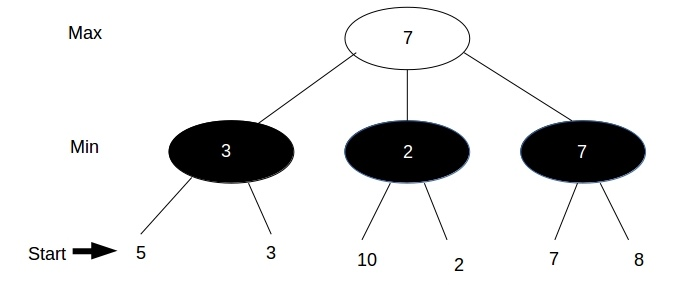
\includegraphics[width=16cm]{graphics/MinMax.jpg}
  \caption{Min-Max}
  \label{FIG:MINMAX}
\end{figure}

\subsubsection{Code}
\label{SUBSUBSEC:AICODE}

Die theoretischen Grundlagen zum Verständnis des Algorithmus sollten nun geklärt sein.\\
Die KI besteht aus zwei Klassen, AI und AILogic. AI wird als neuer Thread ausgeführt. \\
Der nachfolgende Code stellt die AI als Pseudo-Code-Dokumentation dar.\\
Die Klasse AI bekommt eine ArrayList der besten Züge (von AILogic) und führt den letzten Eintrag der Liste aus. Falls sich herausstellen sollte, dass die KI dadurch den eigenen König bedroht, nimmt sie den vorletzten Zug. Wenn dieser Zug wiederum den König in eine bedrohte Situation bringt, wird der drittletzte Eintrag ausgeführt. Dies geht solange weiter, bis alle Einträge der ArrayList aufgebraucht sind. Siehe Pseudo-Code:

\lstset{language=Java}
\begin{lstlisting}
	public class AI extends Thread{
		public void run(){
			AILogic AIL = initialisiere AILogic()
			AIL.alphaBeta() - initialisiert die AI-Berechnung in welcher der bestmoegliche Zug festgestellt wird
			
			Move = bekomme alle moeglichen Zuege der AI
			
			for(alle berechneten Zuege - beginnend beim letzten){
				...
				Der Zug wird getaetigt
				...
				if(Wenn der AI-Koenig nicht im Schach steht){					
					break;
				}
				...
				Der Zug wird rueckgaengig gemacht
				...
			}
			
			Schachmatt ueberpruefen
		}
	}	
\end{lstlisting}
\newpage
\textbf{Klasse AI-Logic:} Die Klasse AI-Logic führt die KI-Berechnung durch. Eingeteilt wird diese in die Methoden alphaBeta, aplphaBetaHelper, boardEvaluation und die verschiedenen SquareRootTables.\\
AlphaBeta bekommt die Informationen bis zu welcher Tiefe eine Suche stattfinden soll und für welches Team. Dies gibt AlphaBeta der Methode AlphaBetaHelper weiter. \\
 Da der AlphaBeta-Algorithmus durch ein sogenanntes ,,Iterative-Deepening'' modifiziert wurde, wird die weitergegebene Tiefe schrittweise erhöht. \\
 AlphaBetaHelper gibt die Günstigkeit eines Zuges als ,,Float'' zurück. Dies wird über die Methode boardEvaluation ermittelt. Falls die tiefste Ebene erreicht wurde, wird dies sofort zurückgegeben und der Rest des Codes nicht weiter ausgeführt. \\
 Andernfalls werden alle Figuren des Teams ausgewählt und nacheinander die Spielzüge simuliert. Sobald die erste Figur des Teams simuliert wurde, ruft sich der Algorithmus rekursiv mit erhöhter Tiefe und geändertem Team auf, bis die maximale Tiefe erreicht wurde (siehe ~\ref{SUBSUBSEC:MinMax}). \\
 Falls ein Spielzug in der geringsten Tiefe besonders günstig ausfällt, wird dieser in eine ArrayList geschrieben, basierend auf dieser ArrayList wird eine Figur in der AI-Klasse bewegt. \\
 
 
\lstset{language=Java}
\begin{lstlisting}
	public class AILogic{
	
		int MaximaleTiefe
		
		public float alphaBeta(tiefe, Hintergrundmatrix, Team){
			MaximaleTiefe = tiefe
			//Diese beiden Werte werden als Worst- und Best-Case Szenario verwendet.
			alpha = 10000
			beta = -10000
			//Fuer iterative deepening
			for(i=0;i<MaximaleTiefe,i++){
				//Bekommt den Wert des besten Zuges
				beta = alphaBetaHelper(starte bei Tiefe 0, Hintergrundmatrix, alpha,beta)
			}
			
		}	
	
		//der AlphaBeta Algorithmus - zur Zugevaluation 
		public float alphaBetaHelper(tiefe, Hintergrundmatrix, Team, alpha, beta){
			Sum = boardEvaluation(Hintergrundmatrix, Team)
			
			if(Sum bedeutet das feindlicher Koenig geschlagen wird){
				return 20000
			}
			
			if(tiefe >= MaximaleTiefe){
				return Sum
			}
			
			for(X und Y Positionen des Spielfeldes){
				if(Spielfigur an Position X und Y){
					Zuege = AlleMoeglichenZuegeDerSpielfigur
					for(alle Moeglichen Zuege der Figur){
						
						MovePos A = Zug der Figur					
						...
						Den Zug auf das Spielfeld uebertragen
						Spezialzuege werden hier speziell behandelt						
						...
						Sum1 = -alphaBetaHelper(tiefe+1, BackgroundGrid, Teamwechsel, -alpha, -beta)
						...
						Den Zug rueckgaengig machen	
						Spezialzuege werden hier speziell behandelt	
						...
						//groesser fuer den ,,Better-AI'' Mode, groesser gleich fuer den normalen Modus (hier aus Uebersichtsgruenden nicht angefuehrt)
						if(Better-AI && Sum1 > beta){
							beta = Sum1	
							if(Sum1 >= alpha){
								return alpha
							}			
							if(tiefe == 0){
								ZuListeGuterZuegeHinzufuegen(A)						
							}
						}
					}
				}
			}
		return beta			
		}
		
		public float boardEvaluation(Hintergrundmatrix, Team){
			//Fuer die Material Balance
			
			for(X und Y Positionen des Spielfeldes){
				if(Bauer weisses Team){
					100 Punkte zum weissen Team dazu zaehlen
					Punkte entsprechend der Bauerntabelle hinzuzaehlen
					Punkte nach Bauerntabelle hinzuzaehlen
				} else if(Turm weisses Team){
					500 Punkte zum weissen Team dazu zaehlen
					Punkte entsprechend der Turmtabelle hinzuzaehlen
				} else if(Springer weisses Team){
					325 Punkte zum weissen Team dazu zaehlen
					Punkte entsprechend der Springertabelle hinzuzaehlen
				} else if(Lauefer weisses Team){
					300 Punkte zum weissen Team dazu zaehlen
					Punkte entsprechend der Lauefertabelle hinzuzaehlen
				} else if(Dame weisses Team){
					900 Punkte zum weissen Team dazu zaehlen
					Punkte entsprechend der Damentabelle hinzuzaehlen
				} else if(Koenig weisses Team){
					10000 Punkte zum weissen Team dazu zaehlen
					Punkte entsprechend der Koenigtabelle hinzuzaehlen
				}
				
				if(Bauer schwarzes Team){
					100 Punkte zum schwarzen Team dazu zaehlen
					Punkte entsprechend der Bauerntabelle hinzuzaehlen
					Punkte nach Bauerntabelle hinzuzaehlen
				} else if(Turm schwarzes Team){
					500 Punkte zum schwarzen Team dazu zaehlen
					Punkte entsprechend der Turmtabelle hinzuzaehlen
				} else if(Springer schwarzes Team){
					325 Punkte zum schwarzen Team dazu zaehlen
					Punkte entsprechend der Springertabelle hinzuzaehlen
				} else if(Lauefer schwarzes Team){
					300 Punkte zum schwarzen Team dazu zaehlen
					Punkte entsprechend der Lauefertabelle hinzuzaehlen
				} else if(Dame schwarzes Team){
					900 Punkte zum schwarzen Team dazu zaehlen
					Punkte entsprechend der Damentabelle hinzuzaehlen
				} else if(Koenig schwarzes Team){
					10000 Punkte zum schwarzen Team dazu zaehlen
					Punkte entsprechend der Koenigtabelle hinzuzaehlen
				}
			}
		}
		
		Hier folgen die Tabellen fuer die Spielfiguren.
		Diese geben an, wo sich die Figuren am liebsten aufhalten.
		
	}	
\end{lstlisting}
%\lstset{language=German}

%=================================================================================
\clearpage\vfill\newpage{}
%=================================================================================
\section{ChessPI}
\label{SEC:chesspi}

ChessPI ist die Implementierung von JavaChess auf dem Raspberry PI. \\
Wir haben uns die Aufgabe gemacht, das Schachprogramm auf einen Mikro-Computer, wie den RaspberryPI 3b, zu portieren.\\
Die Benutzereingabe soll mittels eines Touchscreens erfolgen, weshalb am RaspberryPI ein Touchscreen angeschlossen wird. Weiteres soll für den ChessPI ein Gehäuse designt und eine Akkusteuerung entworfen werden. \\

\subsection{RaspberryPI}

Der Raspberry PI ist ein vollwertiger Computer, welcher mit einem Linux/GNU OS läuft. Am häufigsten wird die Distribution Raspbian verwendet. \\
Von uns wurde der RaspberryPI 3 Modell B verwendet. Dieser verfügt über eine Quad-Core-1.2 GHz Broadcom-BCM2837-CPU, 1 Giga Byte Random Access Memory.\cite{RaspiSpecs} Dies ist eine deutliche Steigerung gegenüber den vorherigen Modellen, womit das Problem der notwendigen Leistung gelöst wird. \\

\subsection{Touchscreen}

Als Touchscreen wird das ofizielle 7'' Touchscreen Display verwendet. Dies hat eine Auflösung von 800x480 Pixel.    \cite{RaspiScreen} \\
Zusätzlich zum Display gibt es auch eine Adapterplatine, mit welcher der Touchscreen versorgt wird. \\
Halterungen für die Adapterplatine und den Raspberry PI gibt es auf der Rückseite des Touchscreens.

\subsection{Implementierung von JavaChess}
\label{SUBSEC:IMPLEMENTJAVACHESS}

Alle benötigten Schritte beziehen sich lediglich auf die Software- und Stromversorgungs-Implementation, nicht auf die Powerbank- und Gehäuse-Implementation. \\[1ex]
\textbf{Vorbereitung:} \\[2ex]
Es wird ein RaspberryPI 3, eine Mikro SD-Karte mit Raspbian, eine Stromversorgung bzw. eine Powerbank mit einem maximalen Strom von 2,5 A, der 7" Touchscreen, die Adapterplatine, eine Internetverbindung, idealerweise über ein LAN-Kabel und eine USB-Tastatur benötigt. \\

\begin{enumerate}
	\item{Die SD-Karte mit Raspbian wird in den Raspberry PI gesteckt.}
	\item{Die Adapterplatine und der Raspberry PI wird auf den Touchscreen geschraubt.}
	\item{Die Stromversorgung für das Display (VCC \& GND Pin, rotes und blaues Kabel, siehe \cite{RaspiScreen}) wird sichergestellt. Das Flachbandkabel / Datenkabel wird zwischen Raspberry PI und Adapterplatine angebracht.}
	\item{Der Raspberry PI wird an die Stromversorgung angeschlossen, dadurch sollte dieser nun booten und das Display automatisch erkennen.}
	\item{Sobald Raspbian gebootet hat, wird das LAN-Kabel angeschlossen.}
	\item{Nun sollten folgende Befehle in der BASH ausgeführt werden:}
	\begin{enumerate}
		\item{sudo apt-get update}
		\item{sudo apt-get upgrade}
		\item{sudo apt-get install oracle-java8-jdk}
		\item{reboot}
	\end{enumerate}
	\item{Nach der Java Installation muss noch JavaFX ,,dazuinstalliert'' werden, da dies nicht in der Java-Embedded-JDK Serie enthalten ist.}
	\item{Es muss OpenJFX gedownloaded werden. URL: https://chriswhocodes.com/}
	\item{Hier ist die Version für den Raspberry PI zu downloaden (ARMv6)}
	\item{Die gedownloadete OpenJFX-Zip Datei muss im Installationsverzeichnis von Java-JDK8 entpackt werden.}
	\item{In der Commandline wird nun folgender Befehl ausgeführt: unzip openjfx-sdk-overlay-linux-arm6hf.zip -d /<installations-verzeichnis-von-Java \\
	(z.B.: /home/pi/jdk1.8.0\_92)>}
	\item{Das aktuelle Schachspiel wird nun gedownloaded. Achtung: Es muss die ChessPI Version verwendet werden, siehe \ref{SUBSEC:USEDJAVACHESS}}.
	\item{Das Schachspiel wird in ein Verzeichnis nach Wahl abgelegt.}
	\item{Nun kann das Schachspiel gestartet werden, dazu muss der Touchscreen aber noch konfiguriert werden, da sonst ein ,,interessanter'' Offset geschieht. Siehe \ref{SUBSEC:SCREENCONFIG}, bzw. in der Auflistung Punkt 17.}
	\item{Dazu muss zuerst der Touchscreen identifiziert werden: cat /sys/class/input/event1/uevent}
	\item{Bei dem Versuchs-Raspberry PI war dieses Input Device: 0/0/0/0}
	\item{Um das Schachspiel bequem zu öffnen, wird empfohlen ein BASH-Skript zu erstellen. Bei diesem Startvorgang muss noch angegeben werden, an welcher Position OpenJFX die Bildschirmeingaben verwendet werden sollen. Dazu wurden die besten Werte empirisch ermittelt:}
	\item{\#!/bin/bash \\
	sudo java -Dmonocle.input.0/0/0/0.minX=0 -Dmonocle.input.0/0/0/0.minY=0 \\
	-Dmonocle.input.0/0/0/0.maxX=800 -Dmonocle.input.0/0/0/0.maxY=500 \\
	-jar chess.jar
	}
	\item{Das Skript muss noch als ausführbar markiert werden: sudo chmod 777 <skript>}
	\item{Nun das Skript öffnen: sudo ./<skript>}
	\item{Das Schachspiel sollte sich nun öffnen.}
	\item{Damit sich das Spiel direkt nach dem Bootvorgang öffnet, muss ein Skript in dem Ordner /etc/init.d/ erstellt werden. Dieses muss das bereits erstellte Skript ausführen.}
	\item{\#!/bin/bash \\
	/bin/bash <Pfad zum Skript>/<Skript.sh>}
\end{enumerate}

\newpage
\subsection{Wieso reicht die offizielle JDK nicht aus?}

Oracle (Entwickler von Java) hat 2015 die Unterstützung für JavaFX auf \ac{ARM} Plattformen gestrichen. Die OpenJDK besitzt, je nach Version, eine unvollständige bzw. ebenfalls keine JavaFX Unterstüzung für ARM. \\
Dies hat zur Folge, dass JavaChess auf einem RaspberryPI eigentlich gar nicht funktionieren sollte. \\
Aufgrund einiger Recherchen, konnte das Spiel dennoch lauffähig gemacht werden, da zusätzlich zu der offiziellen JavaJDK von Oracle, das OpenJFX Paket installiert wurde. \\
 \\


\subsection{Konfiguration des Touchscreens}
\label{SUBSEC:SCREENCONFIG}

Der Touchscreen muss konfiguriert werden, da OpenJFX nicht weiß, wie groß das Display ist. Dies muss konfiguriert werden, indem beim Starten der .jar diverse Startvariablen angegeben werden. Dies wird in Punkt \ref{SUBSEC:IMPLEMENTJAVACHESS}, Auflistungspunkt 17, behandelt.

\subsection{Verwendete JavaChess Version}
\label{SUBSEC:USEDJAVACHESS}

Die ChessPI-Version unterscheidet sich leicht von der JavaChess-Version. Diese beinhaltet keine Einstellungsmöglichkeiten und weiters kein Speichern/Laden des Spiels.\\
Die KI befindet sich standardmäßig im ,,Better-AI''-Modus auf Schwierigkeitsstufe drei. Bei höheren Schwierigkeitsgraden wäre die erforderliche Performance nicht gegeben.\\[2ex]
Die ChessPI-Version befindet sich aus organisatorischen Gründen nicht auf GitHub. \\Für die ChessPI-Version bitte Alexander Beiser anschreiben (E-Mail: alex@itbeiser.at, GitHub: alexl4123).

%=================================================================================
\clearpage\vfill\newpage{}
%=================================================================================
\section{Akkusteuerung}
\label{SEC:AKKUSTEUR}

Ziel ist es, eine Akkusteuerung zu entwerfen. Diese soll es ermöglichen, den ChessPI auch unterwegs verwenden zu können. \\
Die mobile Spieldauer soll größer als eine Stunde sein. \\[1ex]
Für eine Akkusteuerung gibt es prinzipiell mehrere Möglichkeiten, angefangen bei der Powerbank, über bestimmte ICs bis hin zu einer selbst entwickelten Akkusteuerung. Als Ziel ist eine selbst entwickelte Akkusteuerung definiert.\\

\subsection{Kenngrößen des benötigten Akkumulators}
\label{SUBSEC:AKKU-NEEDS}

Um einen Akku auswählen zu können, muss zuerst einmal definiert werden, was gebraucht wird.\\
\begin{itemize}
	\item{Minimale Betriebsdauer $t_{min}= 1h$}
	\item{Stromaufnahme RaspberryPI-Max: $I=2,5A_{\cite{RaspiPower}}$ - zu beachten ist hierbei, dass die Stromaufnahme bei angeschlossenem Bildschirm ca. zwei Ampere beträgt, falls noch weitere Peripheriegeräte angeschlossen werden, erhöht sich die Stromaufnahme entsprechend.}
	\item{Versorgungsspannung RaspberryPI: $U_V = 5V$}
\end{itemize}

\subsection{Wählen des Akkumulators}
\label{SUBSEC:CHOOSE-AKKU}

Akkumulatoren-Typen gibt es viele, für den Einsatz als RaspberryPI-Versorgung schieden alle aus, bis auf folgende Akkumulatorentypen: Lithium-Ionen (Li-Ion), Nickel-Cadmium (NiCd),  Lithium-Polymer (LiPo) und Lithium-Eisenphosphat ($LiFePO_4$). Jeder dieser Akkutypen bietet verschiedene Vorteile, so bietet LiPo relativ hohe Entladeströme und Li-Ion eine ziemlich hohe Energiedichte \cite{wiki:akku}. \\
Für den Einsatz als Versorgung für den RaspberryPI sollte ein Akku möglichst an die 5V Versorgungsspannung herankommen. Dies in Betracht ziehend, scheiden NiCd (1,2V) und $LiFePO_4$ (3,3V) ebenfalls aus. \\
So bleiben entweder der LiPo (3,7V) oder der Li-Ion (ca. 3,6V) Akkumulator übrig. Von beiden wurden gleichwertige Akkus verglichen, aufgrund der niedrigeren Kosten eines $Li-Ion_{\cite{akku-liion}}$ Akkumulators gegenüber eines $LiPo_{\cite{akku-lipo}}$ Akkumulators, ist die Entscheidung für den Li-Ion Akku gefallen.

\subsection{Der Li-Ion Akku}
\label{SUBSEC:LIION}

Der Lithium-Ionen Akkumulator wird durch das Konstantspannungs-Ladeverfahren geladen. Hierbei wird eine Spannungsquelle mit konstanter Spannung an den Akku angeschlossen. Eingestellt wird die Spannung auf die Standardladespannung des Akkus. Bei 3,7V durchschnittlicher Spannung ist die Ladespannung typ. 4,2 Volt. \\
Die minimal benötigte Kapazität berechnet sich wie folgt, wenn eine Stromaufnahmen von 2,5 Ampere angenommen wird.:
\[Q_{min} = t*I = 1h * 2,5A = 2,5 Ah = 2500 mAh\]
Bei der Verkäuferseite Reichelt wurde ein Akku mit diesen Vorgaben gefunden: \cite{akku-liion}\\
Dieser Akku hat eine maximale Kapazität von 2600 mAh, einen maximalen Entladestrom von 2,5 A und eine Ladespannung von 4,2V. \\[1ex]
Das Datenblatt zu allen technischen Eigenschaften befindet sich auf der Seite von Reichelt \cite{akku-liion} bzw. im Anhang (Siehe Abbildung~\ref{datasheet:akku} auf Seite ~\pageref{datasheet:akku}).

\subsection{Idee der ersten Akkusteuerungsschaltung}
\label{SUBSEC:AKKUSTEUR1}

Die ursprüngliche Idee war es, die Akkus über eine Micro-USB Buchse zu laden und damit den Raspberry PI zu betreiben. Da USB eine Spannung von 5V aufweist, muss diese zum Laden der Akkus auf 4,2 V reduziert werden. Für den Betrieb des Raspberry PIs muss diese Spannung wieder auf 5V erhöht werden. \\
Geladen werden die Akkus parallel und entladen seriell, so muss eine Schaltung entwickelt werden, die eine Umschaltung von seriell auf parallel und umgekehrt, ermöglicht. \\
Weiteres muss die Schaltung für den sicheren Betrieb der Akkus sorgen, so muss diese bei Unter- oder Überspannung abschalten und falls ein Kurzschluss auftritt Schlimmeres verhindern. \\
Eine Akkuladestandanzeige wird mittels zwei LEDs realisiert, die eine schaltet bei 1/3 VCC und die andere bei 2/3 VCC. 

\subsubsection{Laden der Akkus}
\label{SUBSUBSEC:AKKULOAD1}

Durch die Eingangsschaltung der Akkus wird die Versorgungsspannung auf unter 4,2 V gesenkt. Dies geschieht durch zwei in Serie liegende Dioden, eine SI-Diode mit einer Durchschaltspannung von ca. 0,7V und eine Shottky-Diode mit einer Durchschaltspannung von ca. 0,2V. \\
Der Ladestrom darf maximal 2,5A betragen, sollte aber geringer sein, um den Akku nicht zu beschädigen. Als Begrenzung kommt ein Leistungsvorwiderstand zum Einsatz. Dieser hat 4$\Omega$ und begrenzt den Strom auf 1,25 Ampere. \\
Da die Akkus parallel geladen werden, muss dies für jeden Akku einzeln aufgebaut werden. \\
In Punkt \ref{SUBSUBSEC:CIRCUIT-1} befindet sich die Schaltung des ersten Versuches. Folgende Bauteile dieser Schaltung werden für das Laden verwendet:\\
 $D_1,R_{sen1},R_{sen2},D_{s8},D_{S2},S_{I1},S_{I2}, Akku1, Akku2$ \\


\subsubsection{Entladen der Akkus}
\label{SUBSUBSEC:AKKUENTLOAD1}

Das Entladen der Akkus erfolgt durch die Seriellschaltung der Akkus (siehe \nameref{SUBSUBSEC:SERPAR}). Seriell geschalten addiert sich die Spannung der beiden Akkus ,,normal'' auf 7.4 V, maximal auf 8.4V. Diese Spannung wird mittels Step-Down-Converter (LM2596) auf 5 V herunter geregelt.  Dies kann als Versorgung für den Raspberry PI verwendet werden. \\
Die Beschaltung erfolgt gemäß des Datenblattes (Siehe Abbildung ~\ref{datasheet:LM2596-2} auf Seite ~\pageref{datasheet:LM2596-2}). Die Berechnung der beiden Widerstände erfolgt ebenfalls gemäß Datenblatt.
\[R_2 = R_1 \cdot \left(\frac{V_{out}}{V_{ref}} - 1 \right)\]
\[V_{ref} = 1.25 V - R_1 = 1 k\Omega - V_{out} = 5V\]
\[R_2 = 1000*(4-1) = 3 k\Omega\]
Zum Ein- und Ausschalten des Raspberry PIs wird noch ein Schalter verbaut. \\
In Punkt \ref{SUBSUBSEC:CIRCUIT-1} ist die Schaltung des ersten Versuches ersichtlich. Folgende Bauteile dieser Schaltung werden für das Entladen verwendet:\\ $LM2596,C_1,D_{s1},L_1,R_1,R_2,C_2,Schalter,Akku1, Akku2$ \\

\subsubsection{Seriell-Parallel-Schaltung}
\label{SUBSUBSEC:SERPAR}

Die Seriell-Parallel-Umschaltung ermöglicht das Wechseln zwischen dem parallelen Laden und dem seriellen Entladen. Es wird erkannt, ob eine Versorgung angeschlossen ist. Wenn diese angeschlossen ist, schalten die Transistoren so, dass der ohmsche Widerstand zwischen den beiden Akkus zu groß ist, um einen Einfluss auf die Schaltung zu haben.\\
Weiteres wird das Potential des negativen Anschlusses des zweiten Akkus auf Ground gesetzt, um das Laden zu ermöglichen. Die Versorgung wird direkt vor dem Schalter des Ausganges angeschlossen, womit der Akku überbrückt wird, damit er sich nicht gleichzeitig entladen und laden muss. \\[2ex] 
Sobald das Micro-USB-Kabel ausgesteckt wurde, wird VCC mit GND leitend verbunden (Micro USB nicht vorhanden - also Potential undefiniert). Die Verbindung zwischen dem Pluspol von Akku1 und dem Minuspol des zweiten Akkus wird wiederhergestellt. Dabei wird die Verbindung zwischen dem Minuspol des zweiten Akkus und GND aufgehoben, um einen Kurzschluss zu verhindern.  \\
Die Verbindung zwischen dem zweiten Akku und dem LM2596 wird aufgetrennt, um ein Entladen des Akkus zu verhindern. \\
In Punkt \ref{SUBSUBSEC:CIRCUIT-1} ist die Schaltung des ersten Versuches ersichtlich. Folgende Bauteile dieser Schaltung werden für das Entladen verwendet:\\ $T_1,R_{T1},T_3,R_{T3},T_6,R_{T6},T_{m3},T_{m4}, Akku1, Akku2$ \\

\subsubsection{Sicherheit}
\label{SUBSUBSEC:Security1}

Unter Sicherheit werden alle Sicherheitsmaßnahmen verstanden, die eine Fehlfunktion des Akkus verhindern. \\
Dafür gibt es einen Spannungsteiler, welcher alle kritischen Spannungen für Komperatoren zur Verfügung stellt. \\
Die Spannungen sind: 
\begin{itemize}
	\item{Minimale Abschaltspannung: $U_{ref4} = 3 V$}
	\item{Akku zu 33\% geladen:$ U_{ref3}=3,3V$}
	\item{Akku zu 66\% geladen: $U_{ref2} = 3,7V$}
	\item{Maximale Ladespannung erreicht: $U_{ref1} = 4,1V$}
\end{itemize}
Wird die minimale Spannung unterschritten, wird die Verbindung zwischen dem Ausgang und den Akkus gekappt. \\
Wird die maximale Ladespannung erreicht, wird die Verbindung zwischen VCC und den Akkus getrennt. Diese beiden Schutzmechanismen werden für jeden Akku verbaut.\\
In der Schaltung sind drei Vier-Ampere-Sicherungen verbaut, diese sorgen für die nötige Kurzschlusssicherheit.  \\
Die Spannungen $ U_{ref3}=3,3V$ und $U_{ref2} = 3,7V$ geben den Ladestand des ersten Akkus an. Zwei Komperatoren vergleichen fortlaufend die Referenzspannungen mit der Akkuspannung und geben mit Hilfe von zwei LEDs den Akkustand wieder. Da beide Akkus immer den gleichen Ladestand haben sollten, braucht man keine zusätzliche Schaltung für den zweiten Akku.
In Punkt \ref{SUBSUBSEC:CIRCUIT-1} ist die Schaltung des ersten Versuches ersichtlich. Folgende Bauteile dieser Schaltung werden für das Entladen verwendet:\\ $OPV_1, OPV_2,T_2,T_4, T_5,LED_1,LED_2,R_{LED1},R_{LED2},R_{T2}, R_{T4},T_{T5}$ 
\newpage
\subsubsection{Schaltung}
\label{SUBSUBSEC:CIRCUIT-1}
\begin{figure}[H]
  \centering
		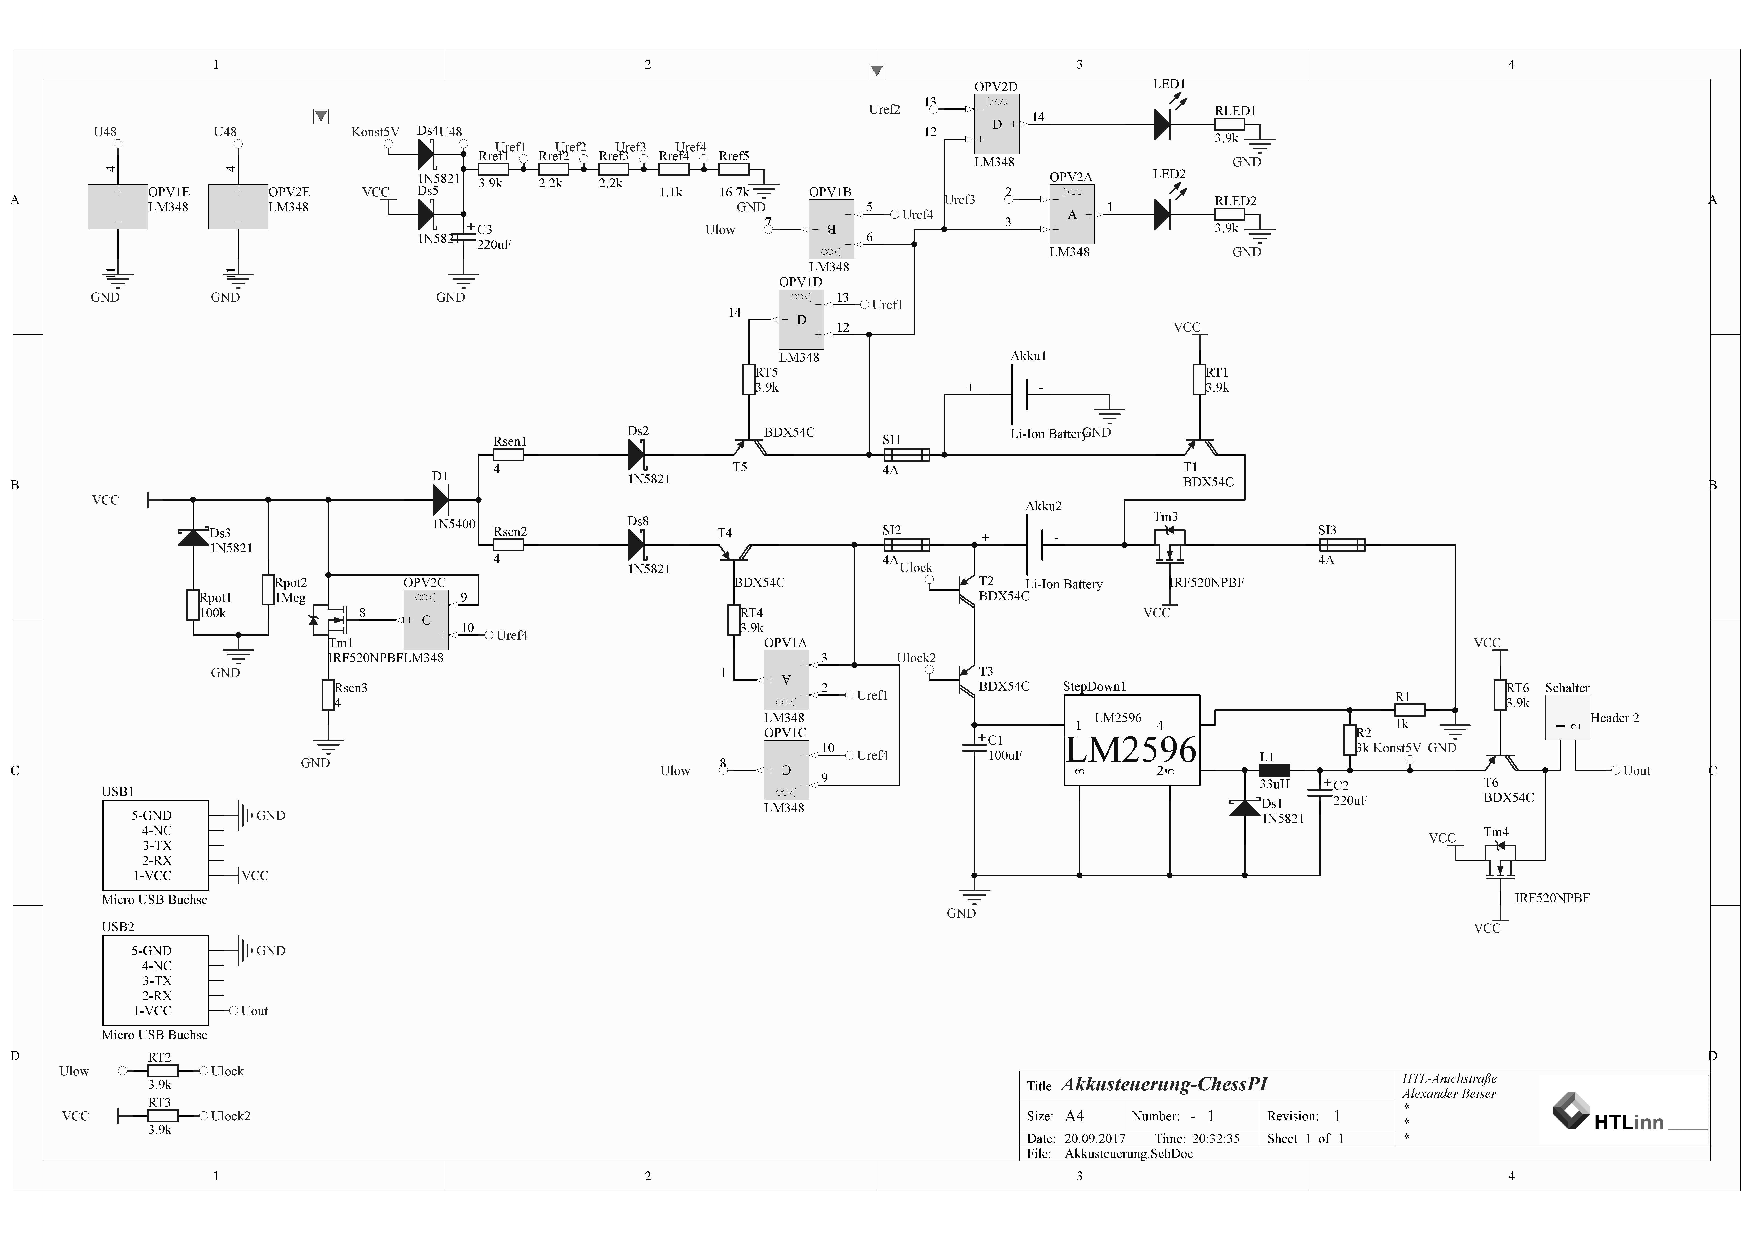
\includegraphics[scale=0.7, angle=90]{graphics/20170920-Shematic.pdf}
		\caption{Die 1. Schaltung}
		\label{fig:circuit1}
\end{figure}

\newpage
\subsubsection{Messung}
\label{SUBSUBSEC:MEASUREMENT1}

Alle Messungen werden auf mehreren Steckbrettern aufgebaut. \\
Die Messung wird in mehrere Phasen gegliedert:
\begin{enumerate}
	\item{Messung der Ausgangsschaltung}
	\item{Messung der Eingangsschaltung}
	\item{Umschalten zwischen den Schaltungen}
	\item{Gesamtschaltungsmessung}
\end{enumerate}
\textbf{Messung der Ausgangsschaltung:}  Es werden ausschließlich die in \ref{SUBSUBSEC:AKKUENTLOAD1} erwähnten Bauteile verwendet. Damit die Akkus nicht gefährdet werden, wird die Messung mit einem Labornetzteil durchgeführt. \\
Dieses wird auf 8,4V (max Akkuspannung) gestellt, anschließend wird der Ausgang gemessen. \\
Die Ausgangsspannung beträgt, wie gefordert, 5V.
Der maximale Ausgangsstrom beträgt mit $T_6$ lediglich 2,0 Ampere, ansonsten 3,2 Ampere. $T_6$ wird hierbei voll ausgesteuert. Zwei Ampere reichen für den RaspberryPI ohne Peripherie, aber mit Display aus. \\
Anschließend wird die Messung mit den Akkus wiederholt, wobei sich das Ergebnis nicht wesentlich ändert.\\[2ex]
\textbf{Messung der Eingangsschaltung:} Es werden ausschließlich die in \ref{SUBSUBSEC:AKKULOAD1} erwähnten Bauteile verwendet. Die Akkus werden sofort eingebaut. Als VCC wird ein Labornetzteil verwendet, welches auf VCC=5V eingestellt wird. \\
Die Messung der Spannungspunkte ergibt das jeweils gewünschte Ergebnis. \\
Der Ladestrom ist aber viel zu niedrig, 2 mA. Zu Testzwecken werden die Sicherheitstransistoren $T_4$ und $T_5$ ausgebaut. Ohne diese beiden Transistoren kommt man auf einen maximalen Eingangsstrom von etwa 25 mA, was ebenfalls zu niedrig ist. \\
Es werden noch mehrere Versuche unternommen, die Schaltung zu retten, was aber nicht gelingt. Somit wird eine komplett neue Eingangsstufe entworfen, siehe hierfür auch die \nameref{SUBSEC:AKKUSTEUR2} (\ref{SUBSEC:AKKUSTEUR2}).


\subsection{Idee der zweiten Akkusteuerungsschaltung}
\label{SUBSEC:AKKUSTEUR2}

Die zweite Akkusteuerungsschaltung unterscheidet sich primär von der ersten in der Eingangsschaltung bzw. der Akkuladeschaltung. Diesmal sind die Akkus ständig in Serie geschalten. Die Sicherheitsvorkehrungen wurden reduziert, sind aber immer noch ausreichend.

\subsubsection{Laden der Akkus}
\label{SUBSUBSEC:AKKULOAD2}

Das Micro-USB-Kabel hat wiederum 5V Versorgungsspannung. Die beiden Akkus sind in Serie geschaltet, weshalb die Ladespannung 8,2V (2*4,1V) betragen muss. Diese Spannung wird durch einen StepUp Converter vom Typ LT1370 erreicht. Dieser ist ein verstellbarer Step-Up-Down-Converter. \\
Die Beschaltung des ICs und die Formel zur Berechnung der Widerstände wird wiederum aus dem Datenblatt entnommen (Siehe Abbildung ~\ref{datasheet:LT1370-2} auf Seite ~\pageref{datasheet:LT1370-2}). \\
\[V_{out}=8,2V;V_{ref}=1,245V;R_{SU2}=10k\Omega\]
\[V_{out}=V_{ref} \cdot \left( 1 + \frac{R_{SU1}}{R_{SU2}} \right)\]
\[R_{SU1} = R_{SU2} \cdot \left( \frac{V_{out}}{V_{ref}} - 1 \right) = 55,8 k\Omega \rightarrow E-12 \rightarrow R_{SU1} = 56 k \Omega\]
Dieses Widerstandsverhältnis transformiert die Spannung von 5V auf 8,2V, wodurch die in Serie geschalteten Akkus geladen werden können.  \\
In Punkt \ref{SUBSUBSEC:CIRCUIT-2} ist die Schaltung des zweiten Versuches ersichtlich. Folgende Bauteile dieser Schaltung werden ausschließlich für das Laden verwendet:\\ $LT1370,C_{SU1},C_{SU2},C_{SU3}, L_{SU1},R_{SU1},R_{SU2},R_{SU3},D_{SU1}$ 

\subsubsection{Entladen der Akkus}
\label{SUBSUBSEC:AKKUENTLOAD2}

Die Entladeschaltung der zweiten Schaltung entspricht exakt der Entladeschaltung des ersten Versuches (siehe: \nameref{SUBSUBSEC:AKKUENTLOAD1} (\ref{SUBSUBSEC:AKKUENTLOAD1})).\\
In Punkt \ref{SUBSUBSEC:CIRCUIT-2} ist die Schaltung des zweiten Versuches ersichtlich. Folgende Bauteile dieser Schaltung werden für das Laden verwendet:\\ $LM2596,D_{S1},L_{SD1},C_{SD2},R_{SD1},R_{SD2}$. 

\subsubsection{Sicherheit}
\label{SUBSUBSEC:Security2}

Als Sicherheit wird wiederum ein Über- und Unterladeschutz verwendet. So gibt es eine automatische Abschaltung, wenn der Akku vollgeladen oder entladen ist. Die Überwachung greift für jeden Akku einzeln. Dies geschieht über Komperatoren, aber nur einen Transistor. Dieser sperrt, wenn der Schutz greift und ist geöffnet, wenn der Akku geladen oder verwendet werden darf. \\
Um den Schutz beider Akkus zu ermöglichen, ist in der Serienschaltung eine Subtrahiererschaltung eingebaut. Die Differenz dieser Schaltung ergibt den momentanen Ladezustand des zweiten Akkus.\\
Die Referenzspannungen der Komperatoren ergeben sich aus einem Spannungsteiler zu:
\begin{itemize}
	\item{$V_{41} = 4,1V$}
	\item{$V_3 = 3V$}
\end{itemize}
\subsubsection{Messung}
\label{SUBSUBSEC:MEASUREMENT2}

Die Ausgangsschaltung wurde schon in \ref{SUBSUBSEC:MEASUREMENT1} geprüft und kann somit ausgelassen werden.  \\
Das Hauptaugenmerk liegt auf der Eingangsstufe, welche die erste Schaltung nutzlos gemacht hat. \\[1ex]
\textbf{Eingangsschaltung: }Die Messung der Eingangsschaltung erfolgt auf einem Steckbrett. VCC wird mittels eines Labornetzteils auf 5V eingestellt. \\
Die Spannungslevel stimmen bei allen Messpunkten. Der Eingangsstrom ist aber wiederum viel zu niedrig (10 mA mit $T_1$, ohne 50 mA). \\
\textbf{Sicherheit:} Es wird überprüft, ob die Sicherheitsabschaltung funktioniert. Dazu wird anstelle der Akkus ein Labornetzteil geschalten, welches einmal auf 8V $U_{A2}$ und einmal auf 2,5V $U_{A2}$ eingestellt wird. Durch diese Einstellung wird der Transistor $T_1$ hochohmig. \\
Die Schaltung kann somit theoretisch als sichere Ladeschaltung verwendet werden. Das Laden eines Akkus dauert allerdings eine Woche. Da das Entwickeln einer neuerlichen Schaltung aufgrund zeitlicher Beschränkungen nicht mehr möglich ist, wird eine Einigung mit Prof. Signitzer getroffen. \\
In dieser wird statt eines Akkumulators und einer Schaltung eine Powerbank verwendet. Für technische Daten siehe \ref{SUBSEC:POWERBANK}.

\subsubsection{Schaltung}
\label{SUBSUBSEC:CIRCUIT-2}
\begin{figure}[H]
  \centering
		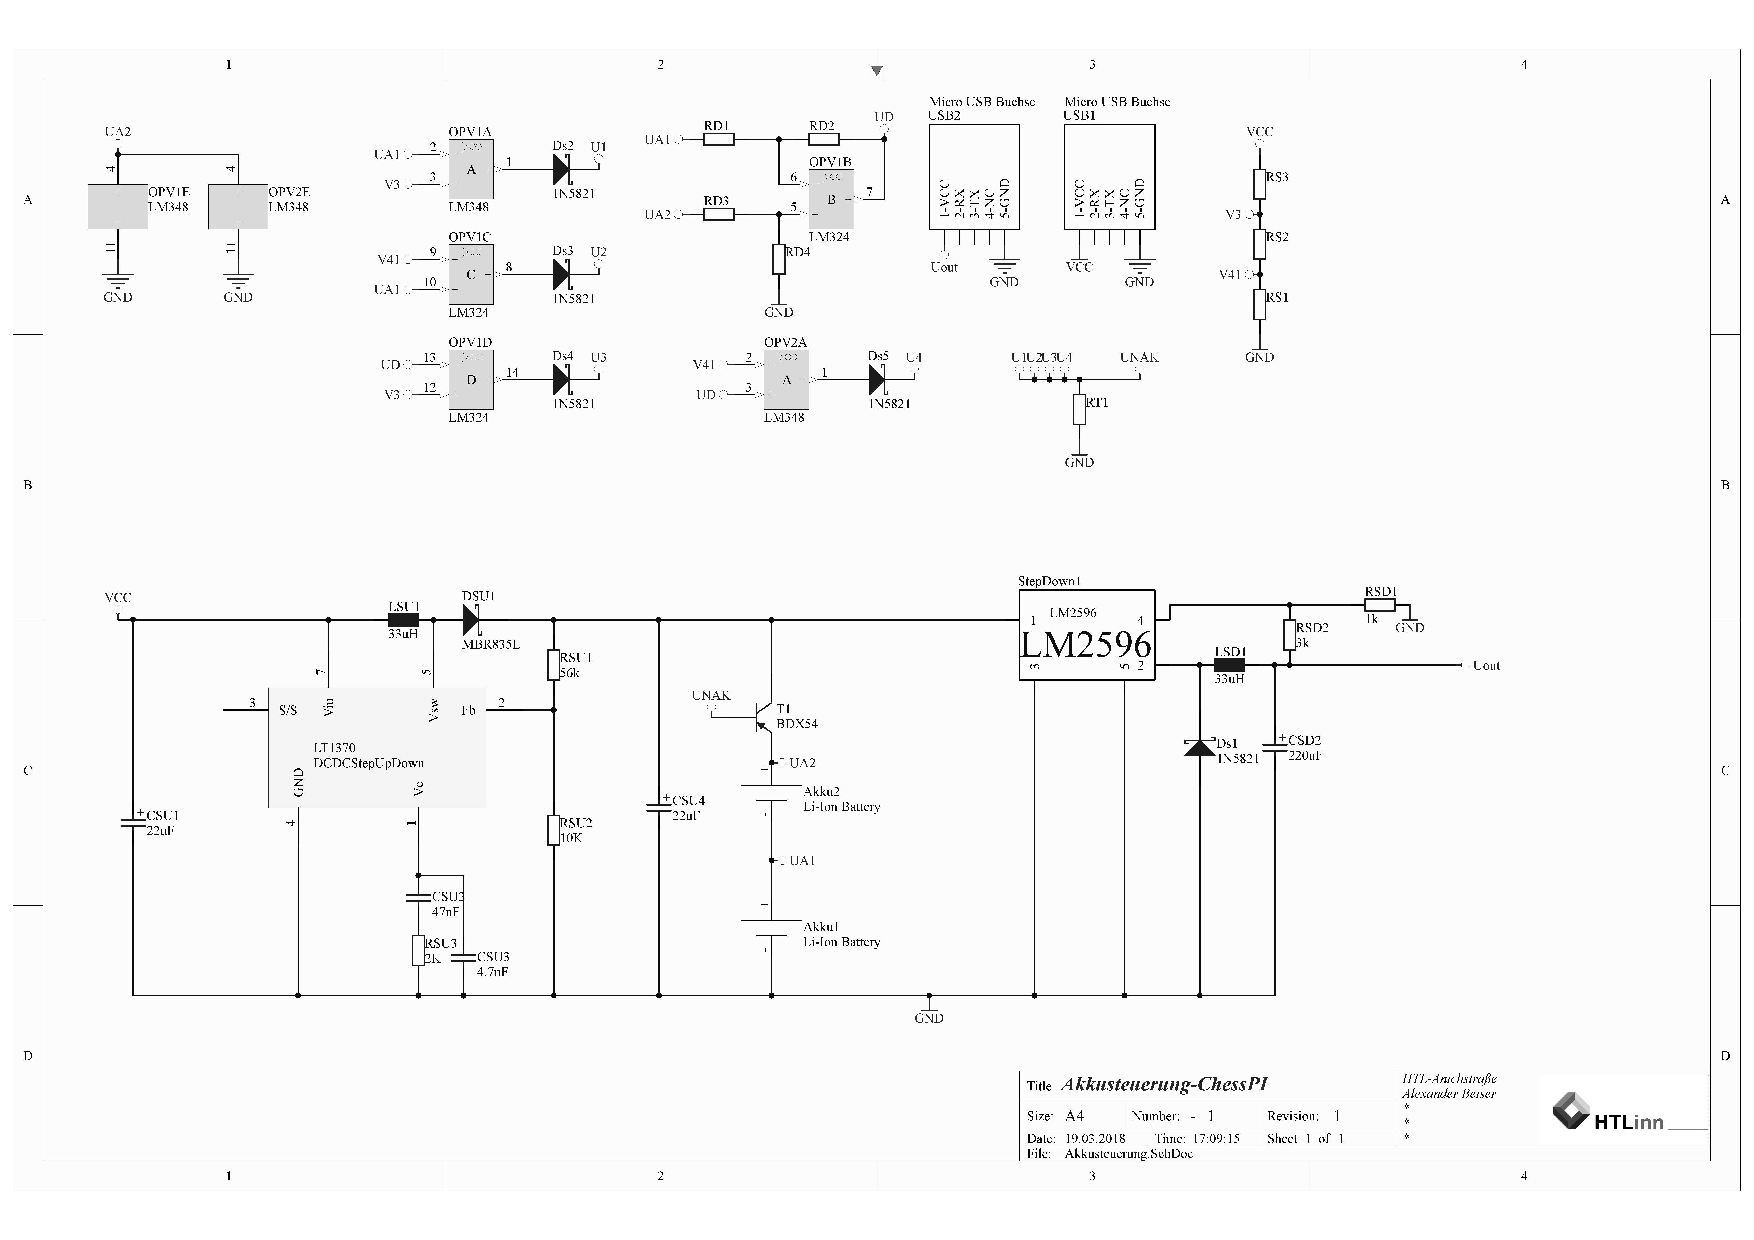
\includegraphics[scale=0.7, angle=90]{graphics/20171104-shematics.pdf}
		\caption{Die 2. Schaltung}
		\label{fig:circuit2}
\end{figure}

\newpage
\subsection{Verwendete Lösung}
\label{SUBSEC:POWERBANK}

Um einen ChessPI-Prototypen rechtzeitig fertigzustellen, wird auf eine selbst entwickelte Schaltung innerhalb des ChessPI verzichtet. Stattdessen soll eine Powerbank verwendet werden. \\
Diese muss folgende Aufgaben erfüllen:
\begin{itemize}
	\item{Min. Entladestrom von 2 A}
	\item{Spielzeit von >1h}
\end{itemize}

Als Powerbank gibt es zwei zur Auswahl stehende Modelle:
\begin{itemize}
	\item{Das Modell RP-PB17 von RAVPower: Dieses erfüllt alle Anforderungen, welche die Powerbank erfüllen muss. Sie hat einen maximalen Ausgangsstrom von 2,4 Ampere und eine Kapazität von 5600 mAh, womit ein Betrieb von bis zu 2,5h möglich ist. Die Größe ist kleiner als der RaspberryPI, womit die Powerbank einfach in das Gehäuse integriert werden kann. \\
Datenblattreferenz für die Powerbank siehe Abbildung ~\ref{datasheet:powerbank} auf Seite ~\pageref{datasheet:powerbank}.
	\item{Das Modell FREEPMULTI10000 von Cellularline - Dieses hat den Vorteil einer erhöhten Kapazität von 10.000 mAh gegenüber den 5600 mAh des anderen Modells. Dafür sind die Abmessungen der FREEPMULTI10000 Powerbank größer, womit ein Einbau in das Gehäuse nur schwer möglich ist.}
}
\end{itemize}
Schlussendlich wird das erste Modell (RP-PB17) verbaut, da das zweite Modell nicht im Gehäuse Platz hat.

%=================================================================================
\clearpage\vfill\newpage{}
%=================================================================================
\section{Gehäuse}
\label{SEC:case}

Aufgabe war es, ein Gehäuse für den RaspberryPI mit Bildschirm und Akkusteuerung zu designen. Anstatt der Akkusteuerung wird nach \ref{SUBSEC:POWERBANK} eine Powerbank verwendet. Für diese sollen noch Ein- und Ausschalter und eine Mikro-USB Buchse für die Versorgung eingebaut werden. \\
Das Gehäuse soll mittels 3D-Drucker erstellt werden, bzw. falls dies nicht in entsprechender Qualität geschehen kann, soll eines in der Kunststoffwerkstätte produziert werden.\\

\subsection{Maße der Bauteile}

Die Maße für den Bildschirm, den Akku und den RaspberryPI können im Anhang \nameref{SEC:DATASHEET} (\ref{SEC:DATASHEET}) gefunden werden.

\subsection{Geplantes mit dem 3D-Drucker gefertigtes Gehäuse}

Das Gehäuse wird nach den vorherigen Kriterien entwickelt.  Als Akkumodell wird das größere verwendet (FREEPMULTI10000).\\
Da das Gehäuse mit einem 3D-Drucker gefertigt werden soll, unterliegt die Fertigung gewissen Beschränkungen. Unter anderem ist ein Gehäuse in der ursprünglich gewünschten Größe nicht möglich, da der Drucker kein Gehäuse von 180x110x50mm, in einer realistischen Zeit und mit wirtschaftlichen Materialverbrauch drucken kann. Dies führt zu einer Aufteilung des geplanten Gehäuses in drei Teile: \\
Die Basis soll auf den RaspberryPI geschraubt werden, darauf soll die Akkuhalterung geklebt werden. Da die Akkuhalterung oben offen ist, wird für diese auch ein Deckel geplant, welcher ebenfalls aufgeklebt wird. \\
Das Gehäuse kann produziert werden, allerdings muss das Aussehen vor einem eventuellen kommerziellen Vertrieb noch auf ein ansprechendes Design geprüft werden. Diese Prüfung hat in unserem Fall ergeben, dass es für Endverbraucher mit großer Wahrscheinlichkeit nicht ansprechend wäre, weshalb wir eine verbesserte Version gefertigt haben (Siehe \ref{SUBSEC:KUNST}).

\begin{figure}[H]
  \centering
		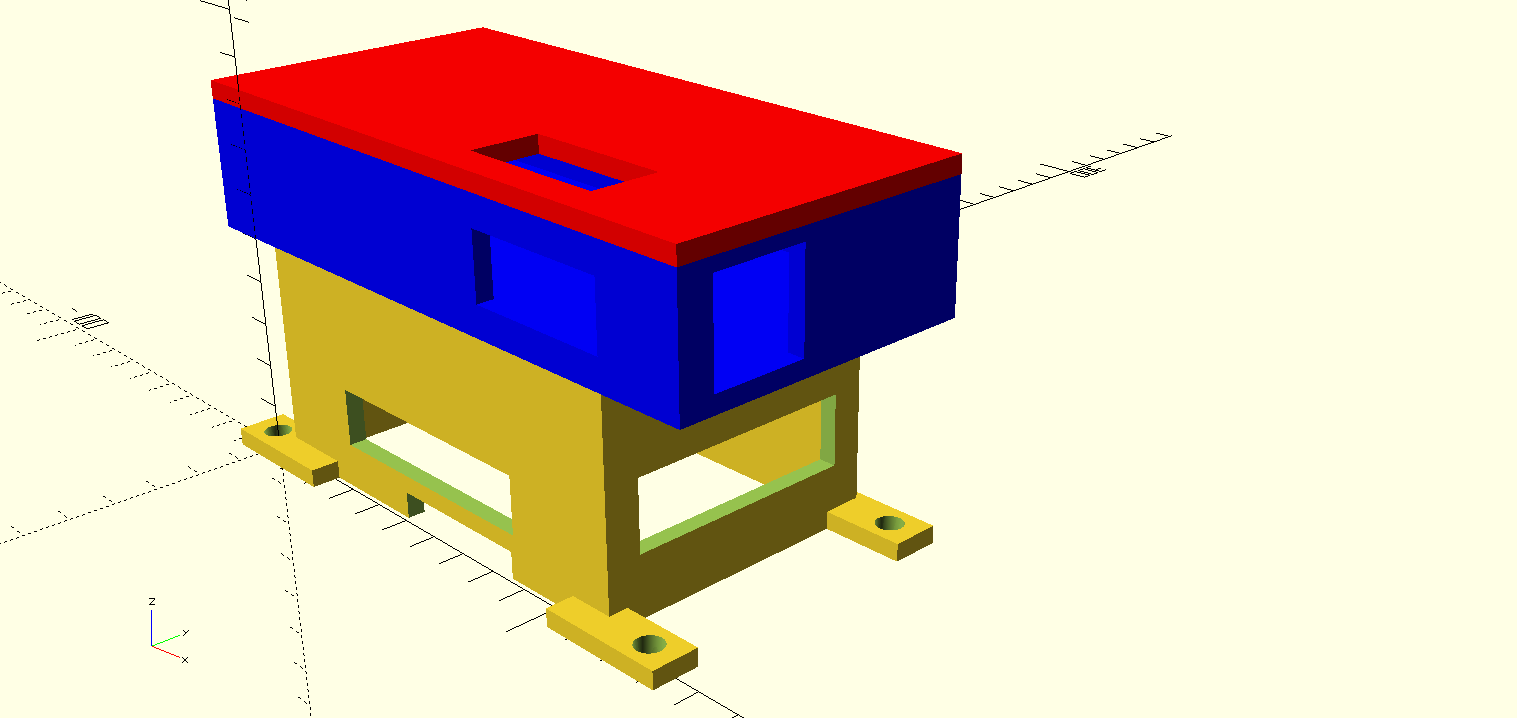
\includegraphics[scale=0.6, angle=90]{graphics/gehaeuse.png}
		\caption{Das Gehäuse in den drei Teilen}
		\label{fig:case-3D}
\end{figure}

\newpage
\subsection{Gehäuse - Kunststoffwerkstätte}
\label{SUBSEC:KUNST}

Als Alternativlösung wird das Gehäuse in der Kunststoffwerkstätte gefertigt. Dieses soll aus poliertem weißem Kunststoff bestehen. \\
Dazu soll noch eine Ladebuchse und ein Schalter verbaut werden. \\
Nach Absprache mit Fachlehrer Strohmaier, welcher mich hier dankenswerter Weise unterstützt hat, wurde das Gehäuse in folgenden Schritten produziert:
\begin{itemize}
	\item{Die Bodenplatte und die beiden Seitenteile werden aus weißem Kunststoff, durch einen Lasercutter, herausgeschnitten.}
	\item{Die Bodenplatte wird gebogen und mit den beiden Seitenteilen verklebt.}
	\item{Es werden vier Löcher in das Gehäuse, für die Befestigungsschrauben gebohrt.}
	\item{Die Platte für den Bildschirm wird ausgeschnitten und die Senkung für den Bildschirm hineingefräst.}
	\item{Die Abstandshalter (innen) werden ausgeschnitten und in beide werden Löcher für die Schrauben gebohrt.}
	\item{Die Löcher für die Mikro-USB-Buchse und für den Ein-Ausschalter werden hineingeschnitten (Lasercutter).}
	\item{Es werden Schrauben für das Verschließen des Displays gesucht. Da es keine >50mm langen M3 Schrauben gibt, wird eine Gewindestange abgeschnitten und das Gehäuse mit einer Mutter befestigt.}
	\item{Damit die Mutter nicht gesehen wird, werden vier Standfüße besorgt, in denen die Mutter Platz hat.}
	\item{Der Akku wird mittels Kabelbindern und selbsthaftenden Pads befestigt.}
	\item{Von diesem geht ein aufgezwicktes USB-Kabel zum Schalter, um das Ein- und Ausschalten zu ermöglichen. \\
Das Laden des Akkus erfolgt mittels Mikro-USB Kabel, von der Mikro-USB Buchse zum Akku.}
\end{itemize}
 
Ein Bild des fertigen ChessPI befindet sich auf der nächsten Seite.

\newpage

\begin{figure}[H]
  \centering
		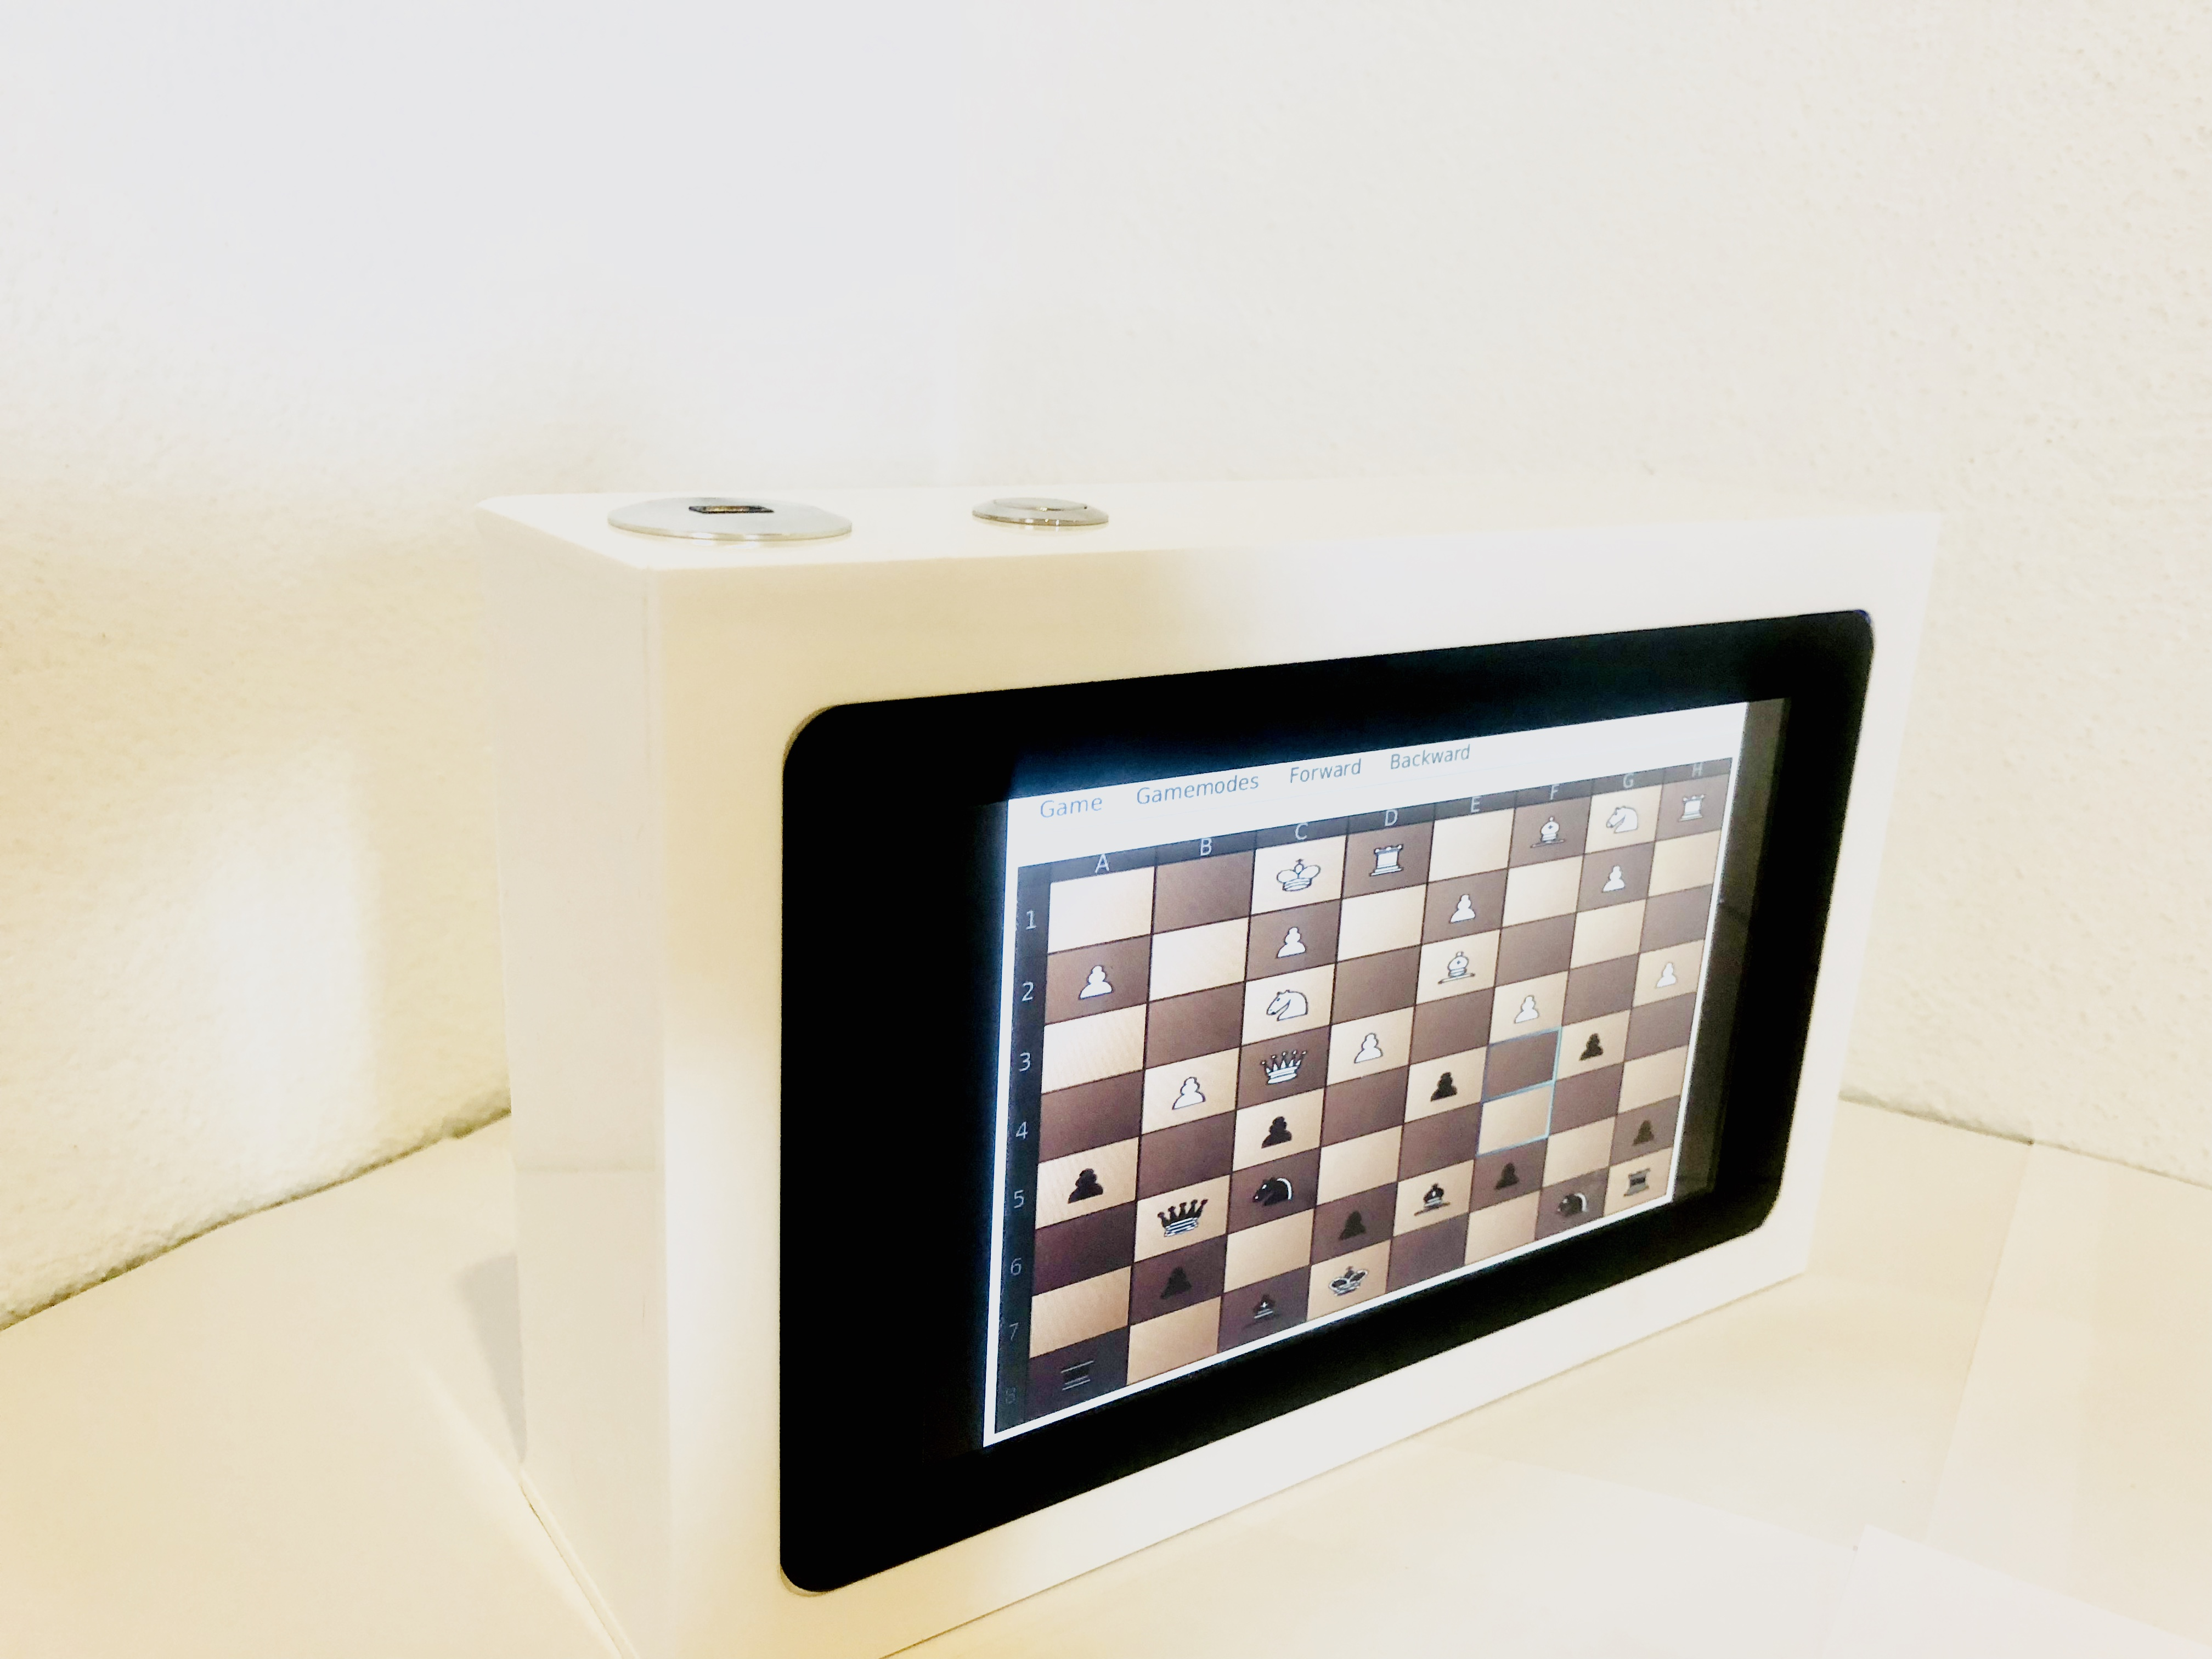
\includegraphics[height =  16cm, angle=90]{graphics/chesspi.jpg}
		\caption{Der ChessPI}
		\label{fig:case}
\end{figure}

%=================================================================================
\clearpage\vfill\newpage{}
%=================================================================================
\section{Android}
\label{SEC:android}

Um das Schachspiel überall spielen zu können, wird geplant, eine Version für die Plattform ,,Android'' zu entwickeln. \\
Diese soll eine vollständige Portierung von JavaChess darstellen und alle diese Funktionen beinhalten. Die Menüführung soll auf Benutzung mittels Wischgesten optimiert werden.\\ [2ex]
Da die Entwicklung der App eine komplett neue Implementierung der graphischen Benutzeroberfläche erfordern würde, und die Entwicklung der App zu einem relativ späten Zeitpunkt geplant ist, zudem die Desktop-Variante noch große Probleme beinhaltet, wird in Rücksprache mit dem Betreuer beschlossen, die Portierung der Android - App in der Frühphase abzubrechen. 

%=================================================================================
\clearpage\vfill\newpage{}
%=================================================================================
\section{Beta}
\label{SEC:beta}

Der letzte Meilenstein war die Beta-Phase. In dieser sollten alle Funktionen des Spiels durch ausgewählte Tester noch einmal auf Herz und Nieren geprüft werden. Die Beta Tester sind deshalb aus verschiedenen Hintergründen ausgewählt worden, zum Beispiel eine professionelle Schachspielerin oder Software-EntwicklerInnen. Dies hat den Vorteil unterschiedliche Nutzerverhalten zu testen. \\[1ex]
Sowohl Alexander Beiser (\ref{SUBSEC:BETAGAME}) als auch Marcel Huber (\ref{SUBSEC:BETALAN}) hatten fünf Tester zu den Punkten:
\begin{enumerate}[I]
	\item{Generelles Spielgefühl}
	\item{Eventuell gefundene Bugs bzw. Verbesserungsvorschläge}
\end{enumerate}

\subsection{AI und Spielmechanik}
\label{SUBSEC:BETAGAME}

\subsubsection*{Chiara Polterauer (Schach-Staatsmeisterin)}
\begin{enumerate}[I]
	\item{Findet das Spiel eigentlich ganz in Ordnung, hat aber ein paar Verbesserungsvorschläge für eine eventuelle Weiterentwicklung des Spiels.}
	\item{Hat die KI im ,,Better-AI'' Modus auf dem maximalen Level geschlagen (bis jetzt einzige TesterIn) und wünscht sich somit eine bessere KI. }
\end{enumerate}

\subsubsection*{Jonas Bangratz}
\begin{enumerate}[I]
	\item{Um hier Jonas Bangratz wörtlich zu zitieren (22.03.2018): ,,Neben einigen Unregelmäßigkeiten, welche die Beta-Version zu diesem Zeitpunkt enthielt, war es für die Software dennoch möglich mir ein relativ gutes Spielgefühl zu vermitteln.''}
	\item{Im Computermodus auf der niedrigsten Schwierigkeitsstufe, war es möglich den feindlichen König zu schlagen. Genauer betrachtet ist der feindliche König auf ein Feld gefahren, dass bedroht wird, wodurch dieser im nächsten Zug geschlagen werden konnte. Dies kann eigentlich gar nicht geschehen, da die KI nie den eigenen König bedrohen würde. Da die KI auf der niedersten Schwierigkeitsstufe aber keine Züge voraus berechnet, weiß diese nicht, dass der König durch diesen Zug bedroht werden kann. Aus diesem Grund wurde die KI mit einem menschlichem Spieler in der Spiellogik vollständig gleichgestellt und darf diesen Zug nun nicht mehr ausführen. Dies hat Performance-Einbußen zur Folge, welche aber verschmerzbar sind. }
\end{enumerate}

\subsubsection*{Nadja Nicolussi}
\begin{enumerate}[I]
	\item{Findet das Design ansprechend und die verschiedenen Spielmodi vernünftig.}
	\item{Annahme: Ein Team hat als letzte Figur nur mehr den König. Dieser ist aber nicht ins Schach zu setzen, er weicht aus. Dies geschieht daher, dass es in der DRAW()-Methode eine Abfrage gibt, ob eine Patt Situation entstanden ist. Diese Abfrage wird erst gestartet, wenn der König die letzte verbleibende Figur ist. Diese Abfrage hatte einen Bug, welcher den König ,,ausweichen'' lies.}
\end{enumerate}

\subsubsection*{Moritz Schnell}
\begin{enumerate}[I]
	\item{Findet das Spielgefühl ziemlich intuitiv.}
	\item{Kompletter Spielabsturz durch einen Logikfehler in der AI Klasse. Die GUI war nicht mehr anklickbar, da das Überschreiben des aktuellen Spielstandes nicht funktioniert, wodurch ein Weiterspielen unmöglich war. Dieser Fehler ist durch ,,Race Conditions'' aufgetreten und wurde behoben.}
\end{enumerate}

\subsubsection*{Alina Schärmer}
\begin{enumerate}[I]
	\item{Hier wird Alina Schärmer wörtlich zitiert:,,Ich finde das Spiel echt gut gelungen.''}
	\item{Annahme: Der Spieler des weißen Teams bewegt einen Bauern im Hot-Seat-Modus, anschließend wird in den KI-Modus (Standard-Einstellungen) gewechselt. Nach neuerlichem Anklicken des Spielfeldes, sollte die KI einen Zug tätigen. Die KI tätigt aber zwei Züge, was nicht erlaubt ist. Dieser Fehler trat durch Race-Conditions beim Setzen des Boolean Team auf und ist mittlerweile behoben. }
\end{enumerate}

\subsection{LAN und GUI}
\label{SUBSEC:BETALAN}

\subsubsection{Josef Scharmer}
\begin{enumerate}
	\item{Findet das Spiel unterhaltsam und ansprechend.}
	
	\item{Joseph Scharmer fand in Zusammenarbeit mit Stefan Pichler einen Bug, der im LAN-Modus verhinderte, dass die Informationspopups bezüglich Schach und Schachmatt angezeigt werden. Dies lag an einer nicht ausgelösten Schach- bzw. Schachmattabfrage beim Empfangen des neuen Spielfeldes. Um das Problem zu lösen, wurden zusätzliche Schach- und Schachmattabfragen beim Empfangen eines Spielfeldes eingebaut.}
\end{enumerate}

\subsubsection{Sabrina Schiestl}
\begin{enumerate}
	\item{Findet das Spielgefühl intuitiv und gelungen.}

	\item{Sabrina Schiestl entdeckte Fehler beim Verändern der Größe des Spielfeldes. In manchen Spielzuständen wurde die graphische Oberfläche beim Verändern der Größe des Fensters nicht richtig mitverändert. Diese Fehler wurden größten Teils behoben. Bei manchen Gelegenheiten wird das Verändern der Fenstergrößte deaktiviert, um die Fehler zu vermeiden. }
\end{enumerate}

\subsubsection{Katharina Weide}
\begin{enumerate}
	\item{Nach den anfänglichen Abstürzen in der Betaphase gefiel ihr das Spielgefühl gut.}

	\item{Katharina Weide stellte bei ihrem ersten Spielstart fest, dass das Spiel direkt abstürzt. Dies lag an einem Crash des Soundplayers, der auf ihrem Betriebssystem nicht verfügbar war. Die Lösung dieses Problems wurde im Kapitel \ref{SUBSUBSEC:SOUNDBUG} behandelt.}
	
\end{enumerate}

\subsubsection{Fabian Thurnes}
\begin{enumerate}
	\item{Lieferte folgendes Statement zum Programm ab: ,,Bei Casual Games ist mir ein besonders intuitives Nutzererlebnis wichtig. Ich freue mich, zum Erfolg dieses Projektes beigetragen zu haben.''}

	\item{Fabian Thrunes war zwar weniger an der Bugfindung beteiligt, half aber sehr bei der Bewertung der Nutzerfreundlichkeit mit und machte Vorschläge diese zu verbessern. Konkret unterbreitete er den Vorschlag für die neue Menüführung.}
\end{enumerate}


%=================================================================================
\clearpage\vfill\newpage{}
%=================================================================================

\section{\sc Benutzerdokumentation}
	Im folgenden Kapitel ist eine Bedienungsanleitung für JavaChess angegeben. Auch mögliche Fehlermeldungen, die das Programm ausgeben kann, werden im Folgendem abgehandelt. 
	
 \subsection{Installationsanleitung}
	Grundsätzlich ist keine Installation von JavaChess notwendig. Zur Ausführung wird allerdings die aktuelle Version der ,,Java Runtime Environment'' oder kurz JRE, benötigt.\\
Um diese zu installieren, öffnet man einen Webbrowser und navigiert zur Homepage von Oracle. Dort wählt man im Menü den Punkt ,,Downloads'' aus. In den darauf folgenden Submenüs navigiert man weiter zum Punkt ,,Java'', und dann zu ,,Java RuntimeEnviroment'' (es kann auch dieser Link verwendet werden: https://java.com/de/download/).  Dort klickt man auf den ,,Download'' Button und wählt die gewünschte Version zum Download aus. 
Die heruntergeladene Datei muss ausgeführt werden. Um die Installation abzuschließen, muss den Anweisungen im Wizard gefolgt werden. \\
Nach der erfolgreichen Installation der JRE kann JavaChess einfach ausgeführt werden.

 \subsection{Benutzung des Spiels}
	
	\subsubsection{Der Hot-Seat-Modus}
	\label{SUBSUBSEC:USERDOCHOTSEAT}
	
 Um ein Spiel zu starten, muss einfach im Titelbildschirm mit der Maus geklickt werden. Das Programm wird automatisch in den ,,Hot-Seat'' - Spielmodus springen.\\
Im ,,Hot-Seat'' - Modus, oder auch lokaler Modus, können zwei Spieler am selben Computer gegeneinander spielen. \\
Um eine Figur zu bewegen, gibt es 2 Möglichkeiten:
\begin{itemize}

	\item{Eine Figur kann durch Klicken bewegt werden. Mit dem ersten Klick wird eine Figur ausgewählt. Daraufhin erscheinen Hilfen, die anzeigen, wohin die Figur bewegt werden kann. Leere Felder, auf die sich die Figur bewegen kann, werden blau umrandet. Felder, auf denen sich eine Figur befindet, die geschlagen werden kann, werden rot umrandet. Mit dem zweiten Klick auf eines der markierten Felder bewegt sich die Figur.}
	
	\item{Die zweite Möglichkeit, eine Figur zu bewegen, funktioniert mittels ,,Drag and Drop''. Die zu bewegende Figur wird angeklickt, die Maustaste wird gehalten. Daraufhin erscheinen wieder die bekannten Hilfen, die im vorhergehenden Punkt erwähnt wurden. Um die Figur nun zu bewegen, wird sie über das gewünschte Feld gezogen und losgelassen.

Wenn ein Spieler in den Zustand ,,Schach'' gerät, wird er mithilfe eines Popups darüber benachrichtigt. Dieses kann mit der vorgesehenen Schaltfläche geschlossen werden.\\
Erreicht ein Spieler den ,,Schachmatt'' - Zustand, so wird er ebenfalls mit einem Popup darüber informiert. Betätigt er auch hier die Schaltfläche, so wird das Popup geschlossen und ein neues Spiel wird gestartet. \\
Um von einem anderen Spielmodus in den Hot-Seat - Modus zurückzukehren, muss der Punkt ,,Hot-Seat'' im Menü ,,Gamemodes'' ausgewählt werden.
	}

\end{itemize}
	
	\subsubsection{Der LAN - Modus}
	\label{SUBSUBSEC:USERDOCLAN}
	
Mithilfe des LAN-Modus, auch Netzwerkmodus oder Onlinemodus genannt, können zwei Spieler auf unterschiedlichen Computern miteinander spielen.\\
Vorraussetzung dafür ist die Konnektivität mit einem Netzwerk, in dem sich beide Computer befinden. \\
Unterschieden wird in diesem Modus zwischen ,,Host'' und ,,Client''. Der Host wartet auf eine eingehende Verbindung, der Client initiiert diese.\\
Um im LAN-Modus zu spielen, wird der Punkt ,,Network'' im Menü ,,Gamemodes'' ausgewählt.\\
Nach dem Auswählen dieses Spielmodus öffnet sich ein Dialogfenster. In diesem gibt es 3 Möglichkeiten zur Auswahl: ,,host'', ,,join'' und ,,abort''. \\
Wird die Schaltfläche ,,host'' ausgewählt, so erscheint ein Wartebildschirm. Auf diesem wird unter anderem die IP-Adresse angezeigt, die der Client zum Verbindungsaufbau benötigt. Während der Wartebildschirm angezeigt wird, wartet das Programm im Hintergrund auf eingehende Verbindungen. Mittels Mausklick kann der Wartevorgang abgebrochen werden. Dies versetzt das Programm zurück in den lokalen Modus. Verschwindet der Wartebildschirm automatisch, so war der Verbindungsvorgang erfolgreich. \\
Wird die Schaltfläche ,,join'' im Dialogfenster ausgewählt, so erscheint ein weiteres Popup. In diesem Popup befindet sich ein Eingabefeld und zwei Schaltflächen.\\
Die Schaltfläche ,,abort'' versetzt das Programm zurück in den Hot-Seat - Modus.\\
Wird die Schaltfläche ,,Ok'' betätigt, so startet der Verbindungsvorgang zu der im Eingabefeld beschriebenen IP-Adresse.\\[2ex]
Sobald eine erfolgreiche Verbindung besteht, kann das Spiel beginnen. Standardmäßig bewegt der Host die weißen Figuren und der Client die schwarzen Figuren. Die Steuerung des Spiels verläuft äquivalent zum Hot-Seat - Modus. Das bedeutet, die Figuren lassen sich sowohl durch Klicks, als auch durch Klicken und Ziehen bewegen. Auch die Informationspopups, die auf Schach- und Schachmattzustände hinweisen, sind im LAN - Modus vorhanden.\\
Um eine bestehende Verbindung zu trennen, muss im Menü ,,Gamemodes'' der Menüpunkt ,,disconnect'' ausgewählt werden. Anschließend befindet sich das Spiel wieder im Hot-Seat - Modus. 

	\subsubsection{Der AI - Modus}
	\label{SUBSUBSEC:USERDOCAI}
	
Der AI - Modus, auch KI - Modus oder Computermodus genannt, ermöglicht es, alleine gegen einen Computergegner zu spielen. \\
Um in diesem Modus zu spielen, muss im Menü ,,Gamemodes'' der Menüpunkt ,,Computer'' ausgewählt werden. Ohne weitere Umwege startet der Modus.\\
Standardmäßig übernimmt der Computer die schwarzen Figuren. \\
Die Steuerung des Spiels verläuft auch hier äquivalent zum Hot-Seat - Modus. Das bedeutet, dass die Figuren auch in diesem Modus durch Klicken oder Drag and Drop bewegt werden können. Auch die bekannten Informationspopups treten in diesem Spielmodus auf.\\
Nachdem ein Zug getätigt wurde, beginnt der Computer, seinen Gegenzug zu berechnen. \textbf{Achtung:} Dieser Berechnungsvorgang kann je nach Rechenleistung des Computers, auf dem das Spiel gestartet wurde, und der Schwierigkeitsstufe der AI, einen längeren Zeitraum in Anspruch nehmen. Um ein optimales Spielgefühl zu gewährleisten wird empfohlen, auf schwacher Hardware eine der niedrigeren Schwierigkeitsstufen auszuwählen. 
\\Um den Computermodus wieder zu verlassen, muss im Menü ,,Gamemodes'' einer der anderen Spielmodi, also der Punkt ,,Network'' oder ,,HotSeat'' ausgewählt werden. 

	\subsubsection{Die erweiterten Optionen}
	\label{SUBSUBSEC:USERDOCSETUP}
	
	Im Menü ,,other'' unter dem Menüpunkt ,,setup'' sind die erweiterten Einstellungen und Anzeigen zu finden. Diese werden in Form eines Popups zugänglich gemacht und sollen dazu dienen, mehr Informationen über das aktuelle Spiel zu erhalten und allgemeine Einstellungen zu verändern. \\
Grob gesagt unterteilt sich das Popup in drei Sektionen: \\
\begin{itemize}

	\item{\textbf{Audio Options}: In dieser Sektion werden Möglichkeiten gegeben, die Lautstärke des Spiels mithilfe eines Schiebereglers zu verändern oder den Sound mithilfe einer Checkbox aus- oder einzuschalten. Zusätzlich wird neben dem Schieberegler die aktuelle Lautstärke angezeigt und es wird eine Schaltfläche angezeigt, mit deren Hilfe ein Testgeräusch abgespielt werden kann. } 

	\item{\textbf{AI Options}: Diese Sektion bietet die Möglichkeit, die Schwierigkeit des Computergegners anzupassen. Auch wird eine Einstellung zur Verfügung gestellt, mit deren Hilfe die Farbe, welche der Computergegner übernimmt, angepasst werden kann. Mit der Checkbox ,,Better-AI'' kann ein alternativer AI-Algorithmus aktiviert werden, der einen noch schwierigeren Gegner bietet. }

	\item{\textbf{Other Information and Options}: Unter dieser Sektion sind Informationen über den aktuellen Rundenstand zu finden und das aktuell ziehende Team wird angezeigt. Aufgrund der Wünsche unserer Betatester wurde die Checkbox ,,Square Board'' eingebaut. Diese hat die Funktion, das Schachfeld auf ein quadratisches Seitenverhältnis zu beschränken.}
	
\end{itemize}

	
	\subsubsection{Alle Menüpunkte}

\begin{itemize}
	\item{\textbf{Game}: \begin{itemize}
			\item{\textbf{New}: Mit diesem Menüpunkt kann ein neues Spielfeld erzeugt werden. Im LAN-Modus steht diese Funktion nicht zur Verfügung.  }
			
			\item{\textbf{Save}: Dieser Menüpunkt ermöglicht es, das aktuelle Schachfeld für einen späteren Zeitpunkt zu speichern. Wenn er ausgewählt wird, öffnet sich je nach laufendem Betriebssystem der entsprechende File - Explorer. Diese Funktion steht im LAN-Modus nicht zur Verfügung. }
			
			\item{\textbf{Load}: Um die gespeicherten Spielfelder wieder laden zu können, wird dieser Menüpunkt verwendet. Auch hier öffnet sich nach dem Auswählen des Punktes der File - Explorer des Betriebssystems. Auch diese Funktion steht im LAN-Modus nicht zur Verfügung.  }
			
			\item{\textbf{Exit}: Dieser Menüpunkt stellt eine  Möglichkeit dar, das Programm zu beenden. Als Alternative kann der Betriebssystemspezifische ,,Close - Button'' verwendet werden.}
		\end{itemize}}
		
	\item{\textbf{Gamemodes}: \begin{itemize}
			
		\item{\textbf{Hot-Seat}: Dieser Menüpunkt erlaubt es, den Hot-Seat - Spielmodus auszuwählen (vgl. \ref{SUBSUBSEC:USERDOCHOTSEAT}).}
	
		\item{\textbf{Network}: Mit dem Auswählen dieses Menüpunktes beginnt die Konfiguration des LAN - Spielmodus (vgl. \ref{SUBSUBSEC:USERDOCLAN}). }
		
		\item{\textbf{Computer}: Durch das Auswählen dieses Menüpunktes startet der AI - Modus (vgl. \ref{SUBSUBSEC:USERDOCAI}). }
		
		\item{\textbf{Launchpad}: Solange der Launchpad - Modus aktiv ist, ist es möglich, die Schachfiguren mithilfe des ,,Launchpad'' zu verschieben. Er funktioniert nur, wenn ein Launchpad verbunden ist. Dieser Modus ist durch eine Kooperation mit der Diplomarbeit ,,Launchpad'', von Alexander Hold und Thomas Klotz, entstanden. Weitere Informationen über das Launchpad sind in deren Arbeit enthalten (siehe GitHub: DarkSunHD - STM32F1 MIDI Serial Bridge).}	
	\end{itemize}}
	
	\item{\textbf{Other}: \begin{itemize}
	
			\item{\textbf{Setup}: Mit dem Anwählen dieses Menüpunktes öffnen sich die erweiterten Optionen und Informationen. Mehr dazu unter \ref{SUBSUBSEC:USERDOCSETUP}. }
			
			\item{\textbf{Draw}: Dieser Menüpunkt wird verwendet, um im Falle eines Patts das Spiel neu zu starten.}
			
	\end{itemize}}
	
	\item{\textbf{Help}: \begin{itemize}

		\item{\textbf{About}: Wenn dieser Menüpunkt ausgewählt wird, öffnet sich ein Popup, in dem Informationen über die Entwickler, die verwendete Lizenz und die GitHub - Repository und das Logo des Spiels angeführt sind. }	
		
		\item{\textbf{Help}: Beim Auswählen dieses Menüpunktes öffnet sich ein weiteres Popup, in dem eine Kurzfassung dieser Anleitung zu finden ist. }	
	
	\end{itemize}}
	
	\item{\textbf{undo}: Mit dieser Schaltfläche ist es möglich, den letzten Zug ungeschehen zu machen. Diese Funktion ist nicht im LAN-Modus verfügbar.}
	
	\item{\textbf{redo}: Um die Aktion des ,,Undo'' Menüpunktes umzukehren, wird dieser Menüpunkt verwendet. }
		
\end{itemize}
 
 \subsection{Fehlermeldungen und Hinweise auf Fehlerursachen}
 
 \subsubsection{Fehler beim Starten des Spiels}
 
  Wenn die ,,.jar - File'' nicht ausgeführt werden kann, überprüfen Sie bitte, ob eine funktionierende Version der ,,Java Runtime Environment'' auf ihrem System installiert ist, und ob Sie über die aktuelle Version von JavaChess verfügen. 
 
 \subsubsection{Fehler beim Speichern eines Spielstandes}
 
Wenn beim Speichern eines Spieles ein Fehler auftritt, erscheint ein Popup mit der Beschriftung ,,File could not be saved!''. Dies kann folgende Ursachen haben:
\begin{itemize}

\item{In dem Dateinamen, unter dem das Feld gespeichert werden sollte, ist ein Sonderzeichen enthalten, das nicht vom Dateisystem unterstützt wird. In diesem Fall muss der Name der zu speichernden Datei angepasst werden. }

\item{Das Programm hat keine Schreibrechte. In diesem Fall muss dem Programm die Berechtigung zum Schreiben gegeben werden, bzw. muss das Programm als Administrator/Superuser gestartet werden. }

\end{itemize}

	\subsubsection{Fehler beim Laden eines Spielstandes}

Wenn beim Laden eines Spieles ein Fehler auftritt, erscheint ein Popup mit der Beschriftung ,,File could not be loaded!''. Dies kann folgende Ursachen haben:

\begin{itemize}

\item{Die Datei, die versucht wird zu laden, ist keine .sav Datei, die vom Programm JavaChess gespeichert wurde. Stellen Sie sicher, dass Sie die richtige Datei ausgewählt haben. }

\item{Die zu ladende Datei wurde verändert und deshalb beschädigt. In diesem Fall ist der Spielstand leider verloren und nicht wiederherzustellen.}


\end{itemize}

	\subsubsection{Fehler im LAN - Modus}
Folgende Fehlermeldungen könne im LAN - Modus auftreten:



\begin{itemize}
 
\item{Wenn eine bestehende Netzwerkverbindung verloren geht, wird ein Informationsbildschirm mit der Meldung ,,The other player disconnected'' angezeigt. Diese Meldung können Sie mit einem Mausklick bestätigen. Im Anschluss kann das Spiel im HotSeat - Modus oder Computer - Modus fortgesetzt werden.} 

\item{Wenn beim Verbinden zu einem Host die Fehlermeldung ,,Connection Failed - the desired Host is not reachable'' auftritt, so ist die eingegebene IP-Adresse zwar gültig, jedoch antwortet der Host nicht. In diesem Fall sollten beide Spieler überprüfen, ob sie sich im selben Netzwerk befinden.}

\item{Wenn beim Verbinden zu einem Host die Fehlermeldung ,,Connection Failed - It seems that something is wrong with the IP address!'' erscheint, so ist die eingegebene IP-Adresse falsch. Bitte überprüfen Sie, ob der Host im Netzwerk existiert und achten Sie darauf, ob die eingegebene Adresse dem Muster ,,127.0.0.0'' entspricht.} 
 
\end{itemize}








%=================================================================================
\clearpage\vfill\newpage{}
%=================================================================================
\renewcommand{\thepage}{\Roman{page}}% Roman for page counter
\setcounter{page}{1}

\setcounter{section}{2000}
\renewcommand\thesection{I}
\renewcommand\thesubsection{\thesection.\Roman{subsection}}
\renewcommand\thesubsubsection{\thesubsection.\Roman{subsubsection}}

	\part*{\sc Anhang}
\section{Abbildungsverzeichnis}\noindent%
\begingroup
\renewcommand{\section}[2]{}
	\listoffigures
\endgroup

%\section{\sc \;}\hfill\\[-23mm]
	%Tabelle 1: Arbeitsaufstellung	9
	\renewcommand\thesection{II}
\section{\sc Tabellenverzeichnis}\noindent%
\begingroup
\renewcommand{\section}[2]{}	
	\listoftables
\endgroup









%=================================================================================
\clearpage\vfill\newpage{}
%=================================================================================
%\renewcommand{\thepage}{\rom{page}}% Roman for page counter
%\vspace*{-8mm}
\renewcommand\thesection{III}
\section{Literaturverzeichnis}
\cmnt{
	{\yhbu
	Beispiele:
	\\[0mm]{\fontsize{10pt}{10pt}\selectfont
	(Übernommen aus dem Leitfaden des BMBF Reife- und Diplomprüfungen März 2014)
	\\[0mm]
	\begin{description*}
	\item[1. Werke eines Autors] Nachname, Vorname: Titel. Untertitel. -
		Verlagsort: Verlag, Jahr. Nachname,
		Vorname: Titel. Untertitel. Auflage - Verlagsort: Verlag, Jahr.
		\\[1mm]Beispiele:
		\\Sandgruber, Roman: Bittersüße Genüsse. Kulturgeschichte der Genußmittel. – Wien:
		Böhlau, 1986. Messmer, Hans-Peter: PC-Hardwarebuch. Aufbau, Funktionsweise,
		Programmierung. Ein Handbuch nicht nur für Profis. 2. Aufl. - Bonn: Addison-Wesley,
		1993.
		\vspace*{2mm}
	\item[2. Werke mehrerer Autoren] Nachname, Vorname; Nachname, Vorname; Nachname, Vorname: Titel.
		Untertitel. Auflage - Verlagsort: Verlag, Jahr.
		\\[1mm]Beispiel:
		\\Bauer, Leonhard; Matis, Herbert: Geburt der Neuzeit. Vom Feudalsystem zur
		Marktgesellschaft. - Mün- chen: Deutscher Taschenbuch Verlag, 1988.
		\vspace*{2mm}
	\item[3. Sammelwerke, Anthologien, CD-ROM mit Herausgeber] Nachname, Vorname (Herausgeber):
		Titel. Untertitel. Auflage - Verlagsort: Verlag, Jahr. Nachname, Vorname: Titel.
		Untertitel. In: Nachname, Vorname (Herausgeber): Titel. Untertitel. Auflage -
		Verlagsort: Verlag, Jahr.
		\\[1mm]Beispiele:
		\\Popp, Georg (Hg.): Die Großen der Welt. Von Echnaton bis Gutenberg. 3. Aufl. -
		Würzburg: Arena, 1979. Killik, John R.: Die industrielle Revolution in den Vereinigten
		Staaten. In: Adams, Willi Paul (Hg.): Die Vereinigten Staaten von Amerika. Fischer
		Weltgeschichte Bd. 30. - Frankfurt am Main: Fischer Taschenbuch Verlag, 1977. Killy,
		Walther (Hg.): Literatur Lexikon. Autoren u. Werke deutscher Sprache. – München:
		Bertelsmann, 1999. (Digitale Bibliothek, 2)
		\vspace*{2mm}
	\item[4. Mehrbändige Werke] Nachname, Vorname: Titel. Bd. 3 - Verlagsort: Verlag, Jahr.
		\\[1mm]Beispiel:
		\\Zenk, Andreas: Leitfaden für Novell NetWare. Grundlagen und Installation. Bd. 1 - Bonn:
		Addison Wesley, 1990.
		\vspace*{2mm}
	\item[5. Beiträge in Fachzeitschriften, Zeitungen] Nachname, Vorname des Autors des bearbeiteten
		Artikels: Titel des Artikels. In: Titel der Zeitschrift, Heftnummer, Jahrgang, Seite
		(eventuell: Verlagsort, Verlag).
		\\[1mm]Beispiel:
		\\Beck, Josef: Vorbild Gehirn. Neuronale Netze in der Anwendung. In: Chip, Nr. 7, 1993,
		Seite 26. - Würzburg: Vogel Verlag.
		\vspace*{2mm}
	\item[6. CD-ROM-Lexika]\hfill
		\\[1mm]Beispiel:
		\\Encarta 2000 - Microsoft 1999.
		\vspace*{2mm}
	\item[7. Internet] Nachname, Vorname des Autors: Titel. Online in Internet: URL: www-Adresse, Datum.
		(Autor und Titel wenn vorhanden, Online in Internet: URL: www-Adresse, Datum auf
		jeden Fall)
		\\[1mm]Beispiel:
		\\Ben Salah, Soia: Religiöser Fundamentalismus in Algerien. Online im Internet:
		URL: >>http:/\slash{}www.hausarbeiten.de\slash{}cgi-bin\slash{}superRD.pl<<,
		22.11.2000. Der Weg zur Doppelmonarchie.
		Online in Internet: URL:
		http:/\slash{}www.parlinkom.gv.at\slash{}pd\slash{}doep\slash{}d-k1-2.htm,
		22.11.2000.
		\vspace*{2mm}
	\item[8. Firmenbroschüren, CD-ROM] Werden Inhalte von Firmenunterlagen verwendet,
		dann ist ebenfalls die Quelle anzugeben.
		\\[1mm]Beispiel:
		\\Digitale Turbinenregler. Broschüre der Firma VOITH-HYDRO GmbH, 2012.
		\vspace*{2mm}
	\item[9. Abbildungen, Pläne] Werden Abbildungen aus einer fremden Quelle
		[z.B. Download, Scannen) in die Diplomarbeit eingefügt,
		so ist unmittelbar darunter die Quelle anzugeben.
		\\[1mm]Beispiel:
		\\Abb. 1: Digitaler Turbinenregler [ANDRITZ HYDRO]
		\vspace*{2mm}
	\item[10. Persönliche Mitteilungen]\hfill
		\\[1mm]Beispiel:
		\\Persönliche Mitteilung durch: König, Manfred:
		Kössler GmbH Turbinenbau am 8. März 2013.
	\item[]{The RaspberryPI Foundation: Power Supply. Online im Internet: }
	\item[2.Akkumulatortypen]{
 	}
	\end{description*}
	}}%yhbu
	}

\begingroup
\renewcommand{\section}[2]{}
\begin{thebibliography}{}
\bibitem{wiki:chess}
    Author = "Wikipedia contributors",
    Titel = "Chess --- Wikipedia{,} The Free Encyclopedia",
    Jahr = "2018",
    URL = "\url{https://en.wikipedia.org/w/index.php?title=Chess&oldid=829981577}",
    Notiz = "[Online; accessed 19-March-2018]"
    
    \bibitem{SkyNet}
    	Author = Mike Klein, Titel = Google's AlphaZero Destroys Stockfish in 100-Game Match, 
    	URL = \url{https://www.chess.com/news/view/google-s-alphazero-destroys-stockfish-in-100-game-match}
	
	\bibitem{SquareTables}
	Author = ,,Abarent'', Titel = Piece Square Table, URL = \url{http://www.chessbin.com/post/Piece-Square-Table}    	
	
	\bibitem{RaspiSpecs}
	Author = The MagPi Magazine, Titel = RASPBERRY PI 3 IS OUT NOW! SPECS, BENCHMARKS \& MORE, 
	UTL = \url{https://www.raspberrypi.org/magpi/raspberry-pi-3-specs-benchmarks/}
	
	\bibitem{RaspiScreen}
	Author = ,,Gordon'', Titel = THE EAGERLY AWAITED RASPBERRY PI DISPLAY, 
	URL = \url{https://www.raspberrypi.org/blog/the-eagerly-awaited-raspberry-pi-display/}
    	
	\bibitem{RaspiPower}
		Author: The RaspberryPI Foundation, Titel: Power Supply,
		URL:\url{https://www.raspberrypi.org/documentation/hardware/raspberrypi/power/README.md},
		Notiz = Online; Stand 19. März 2018
		
	\bibitem{wiki:akku}
	 Author = "Wikipedia",
   Titel = ,,Akkumulator --- Wikipedia{,} Die freie Enzyklopädie'',
   Jahr = "2018",
   URL = "\url{https://de.wikipedia.org/w/index.php?title=Akkumulator&oldid=175107886}",
   Notiz = "[Online; Stand 19. März 2018]"
   
   \bibitem{akku-liion}
   Author = RS-Components,
   Titel = Ansmann Lithium-Akkupacks 3.7V/2600mAh, mit Drahtanschluss,
   URL = \url{https://at.rs-online.com/web/p/lithium-akkus/7760853/?searchTerm=776-0853},
	Notiz = Online; Stand 19. März 2018,
	RS-Best. Nr.: 776-0853,
	Herst. Teile-Nr.: 2347-3003
	
	\bibitem{akku-lipo}
	Author = RS-Components,
	Titel = RS Pro Li-Po Akku 3.7V, 2000 mAh, mit Drahtanschluss,
	URL = \url{https://at.rs-online.com/web/c/batterien/akkus/lithium-akkus/?applied-dimensions=4294830943},
	Notiz = Online; Stand 19.März 2018,
	RS-Best Nr.: 125-1266
	
	\bibitem{pragmatic}
	Author 1 = Andrew Hunt, Author 2 = David Thomas,
	Titel = The Pragmactic Programmer, Untertitel = from journeyman to master,
	Verlag = Addison-Wesley, Verlagsort = Crawfordsville, Indiana, United States of America, 
	Jahr = 2000

	
\end{thebibliography}
\endgroup


%=================================================================================
\clearpage\vfill\newpage{}
%=================================================================================
\renewcommand\thesection{IV}
\section{Abkürzungen}
\label{SEC:ACRONYMS}

\begin{acronym}[acronyms]
\acro{PC}{Personal Computer}
\acro{HTL}{Höhere Technische Lehranstalt}
 \acro{GUI}{Graphical-User-Interface}
 \acro{GNU}{GNU's Not Unix}
 \acro{LAN}{Local Area Network}
 \acro{AI}{Artificial-Intelligence}
 \acro{vgl.}{vergleiche}
 \acro{dt.}{zu Deutsch}
 \acro{engl.}{englisch}
 \acro{App.}{Application}
 \acro{ARM}{Advanced RISC Machine}
\end{acronym}








%=================================================================================
\clearpage\vfill\newpage{}
%=================================================================================
\renewcommand\thesection{V}
\section{\sc Pflichtenheft}
\label{SEC:PFLICHTENHEFT}
\vfill
	\begin{center}\begin{huge}
			\textbf{Pflichtenheft für die Diplomarbeit}\\ \vspace{1cm}
			\textbf{JavaChess, ChessPI AndChess}
	\end{huge}\end{center}
\vfill
\newpage

\subsection{\sc JavaChess Konzept}

Das Programm ist als 2D Schachspiel konzipiert. Basierend auf Java und JavaFX wird das Spiel entwickelt. \\
Das Spiel soll online spielbar gemacht werden, aber auch über einen Einzelspielermodus verfügen. Dieser Einzelspielermodus beinhaltet zudem eine selbst entwickelte künstliche Intelligenz. \\
Die grafische Oberfläche setzt sich aus einem selbst designten Schachbrett, Bedienflächen und aus Opensource-Quellen stammenden Ressourcen für die Figuren zusammen.\\
Selbstverständlich sollen alle möglichen Züge implementiert- und ein passender Schachmatt-Algorithmus entwickelt werden. \\
Auf eine ressourcenschonende Zugberechnung soll besonderer Wert gelegt werden, da die künstliche Intelligenz auf denselben Zugmechanismus zugreift, wie der menschliche Spieler. \\
Die Bedienung des Programms soll auf mehrere Arten möglich sein:  mittels Click to Click* und Drag and Drop.\\
*Click-to-Click: Spieler A klickt auf Feld d7 – dann auf Feld d6 – Figur bewegt sich von d7 nach d6.

\subsection{Einzubauende Features}

\subsubsection{JavaChess (Desktop Version - Windows)}

\begin{enumerate}
	\item{GUI}
	\begin{enumerate}
		\item{2D Darstellung des Schachbretts}
		\item{Bedienflächen, in Menüs geordnet}
		\item{Spielstand Indikatoren}
	\end{enumerate}
	\item{Programmlogik}
	\begin{enumerate}
		\item{Zugfunktion}
		\item{Schachmatt-Algorithmus}
		\begin{enumerate}
			\item{Es soll auf die Übersichtlichkeit des Programmcodes geachtet werden}
			\item{Die Kommentare des Programmcodes sollen auf Englisch erfolgen}
		\end{enumerate}
	\end{enumerate}
	\item{Künstliche Intelligenz}
	\begin{enumerate}
		\item{Im Einzelspielermodus ist es möglich, gegen eine selbst entwickelte künstliche Intelligenz zu spielen.}
		\item{Die Evaluierung des besten Zuges der künstlichen Intelligenz erfolgt mithilfe eines abgeänderten Min-Max-Algorithmus.}
	\end{enumerate}
	\item{Netzwerk}
	\begin{enumerate}
		\item{Austausch der Spieldaten über ein Local Area Network.}
	\end{enumerate}
\end{enumerate}

\subsubsection{ChessPI (Raspberry PI 3)}

\begin{enumerate}
	\item{Für einen 7‘‘ Touchscreen optimierte Spielerfahrung}
	\item{Optimierung der künstlichen Intelligenz für Niedrigleistung}
	\item{Eigenentwickeltes Gehäuse, welches mithilfe eines 3D-Druckers gebaut wird}
	\item{Selber entwickelte Akkuansteuerungsschaltung und Einbau des Akkus innerhalb des Gehäuses}
\end{enumerate}

\subsubsection{AndChess (Android)}

\begin{enumerate}
	\item{Vollständig portierter Programmcode für Android basierte mobile Geräte}
	\item{Angepasste GUI für eine bessere Bedienung auf mobilen Geräten}
\end{enumerate}

\subsection{Appendix}
\subsubsection{Vorhandene Bugs}

Hier werden alle bekannten Bugs gelistet, welche behoben werden sollen:

\begin{itemize}
	\item{Schachmatt-Algorithmus gibt, außer in einem bestimmten Fall, nur Schach aus. Dieser bestimmte Fall tritt ein, wenn zwei gegnerische Figuren den König bedrohen.}
	\item{Die Züge Rochade, En Passant, Bauerntausch und der Doppelzug des Bauern, falls dieser sich noch nicht bewegt hat, sind nicht eingebaut.}
	\item{Die Züge des Läufers und der Dame haben den Fehler, falls diese diagonal ziehen, sind auch illegale Züge erlaubt. Z.B.: Lc8 -> Le6}
	\item{Es gibt keine Feststellung, ob Team1 oder Team2 am Zug ist, beide funktionieren immer.}
	\item{Falls es zu einer ,,Schachsituation'' kommt, kann unter besonderen Bedingungen eine Endlosschleife entstehen, die das Programm abstürzen lassen kann.}
\end{itemize}

\renewcommand\thesection{VI}
\section{Datenblätter}
\label{SEC:DATASHEET}



\begin{figure}[H]
  \centering
		\includegraphics[scale=1.5, angle=90,page=2]{graphics/powerbank.pdf}
		\caption{Datenblatt Powerbank}
		\label{datasheet:powerbank}
\end{figure}

\begin{figure}[H]
  \centering
		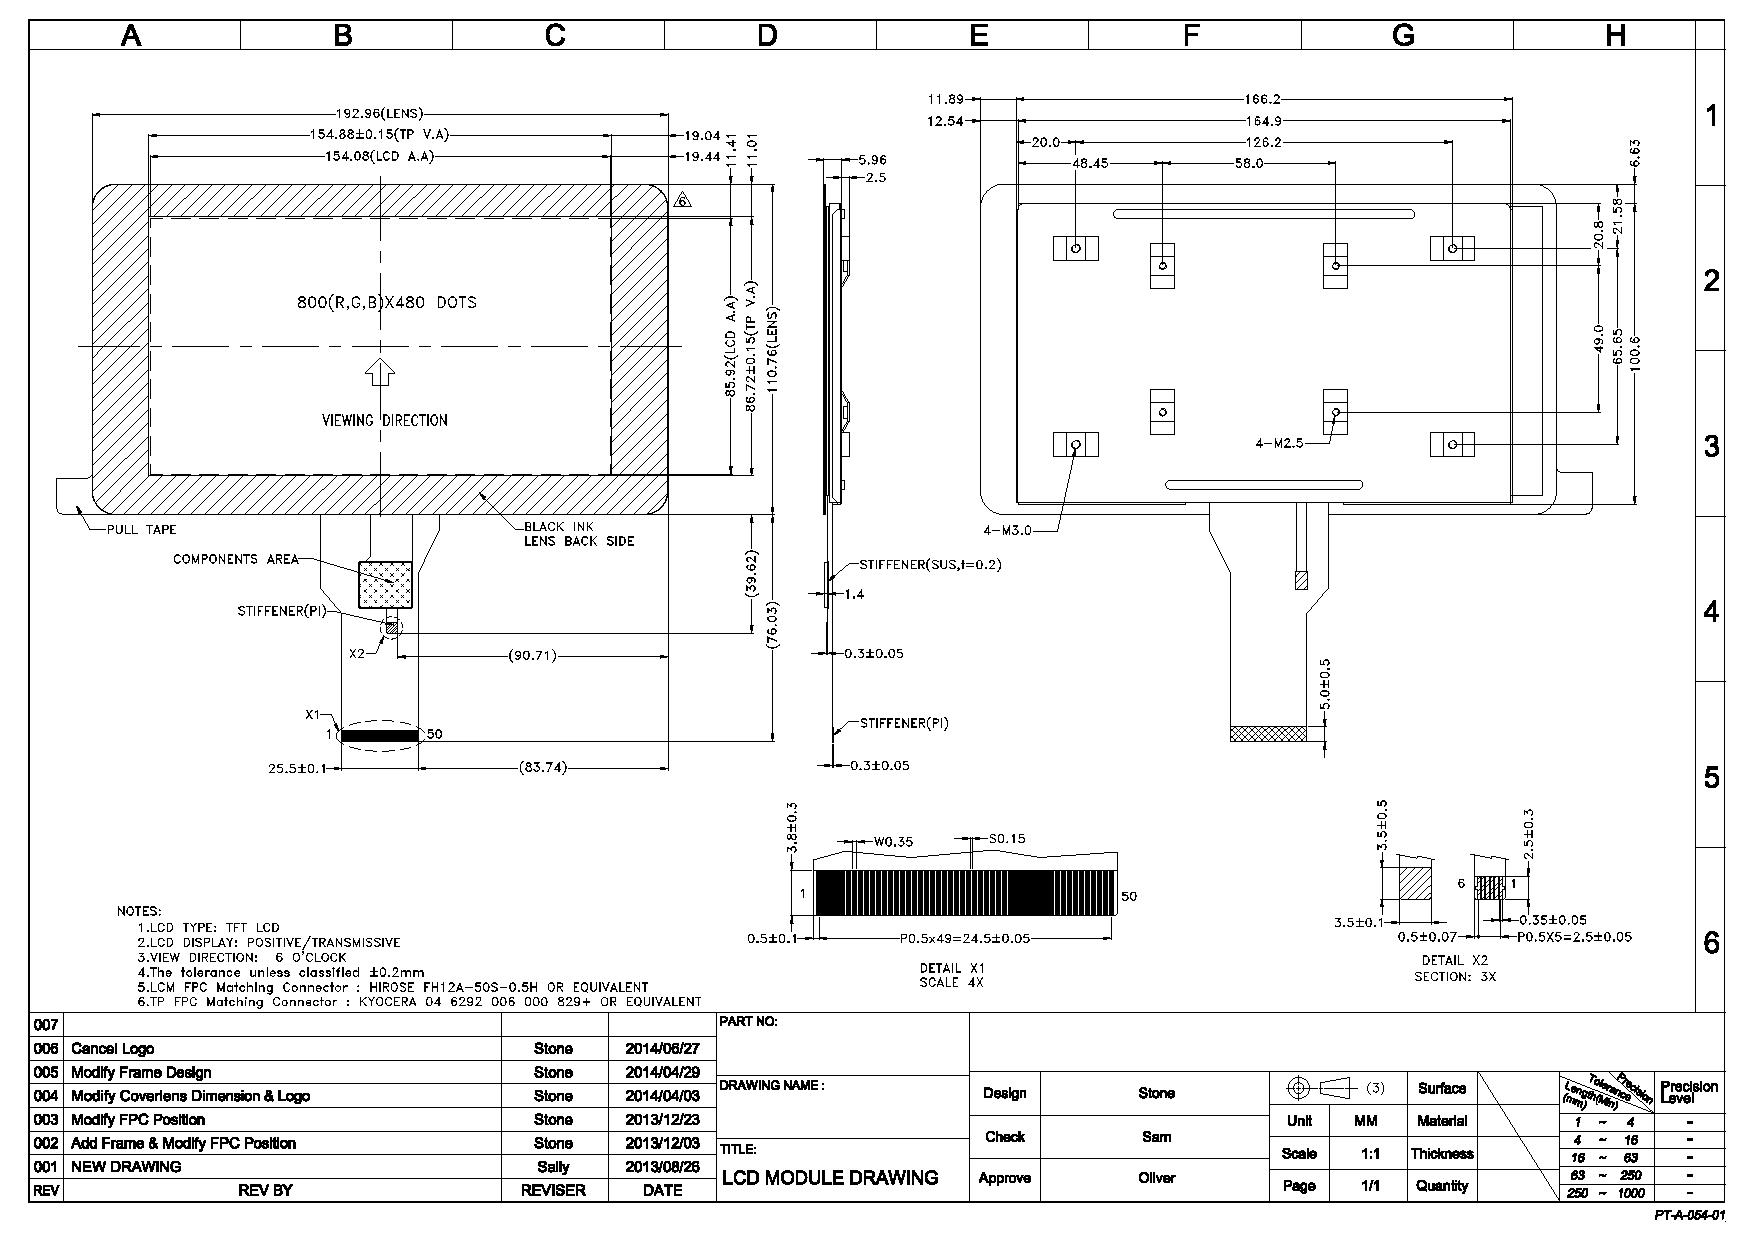
\includegraphics[scale=0.7, angle=90]{graphics/screen.pdf}
		\caption{Datenblatt RaspberryPI Bildschirm}
		\label{datasheet:raspiscreen}
\end{figure}

\begin{figure}[H]
  \centering
		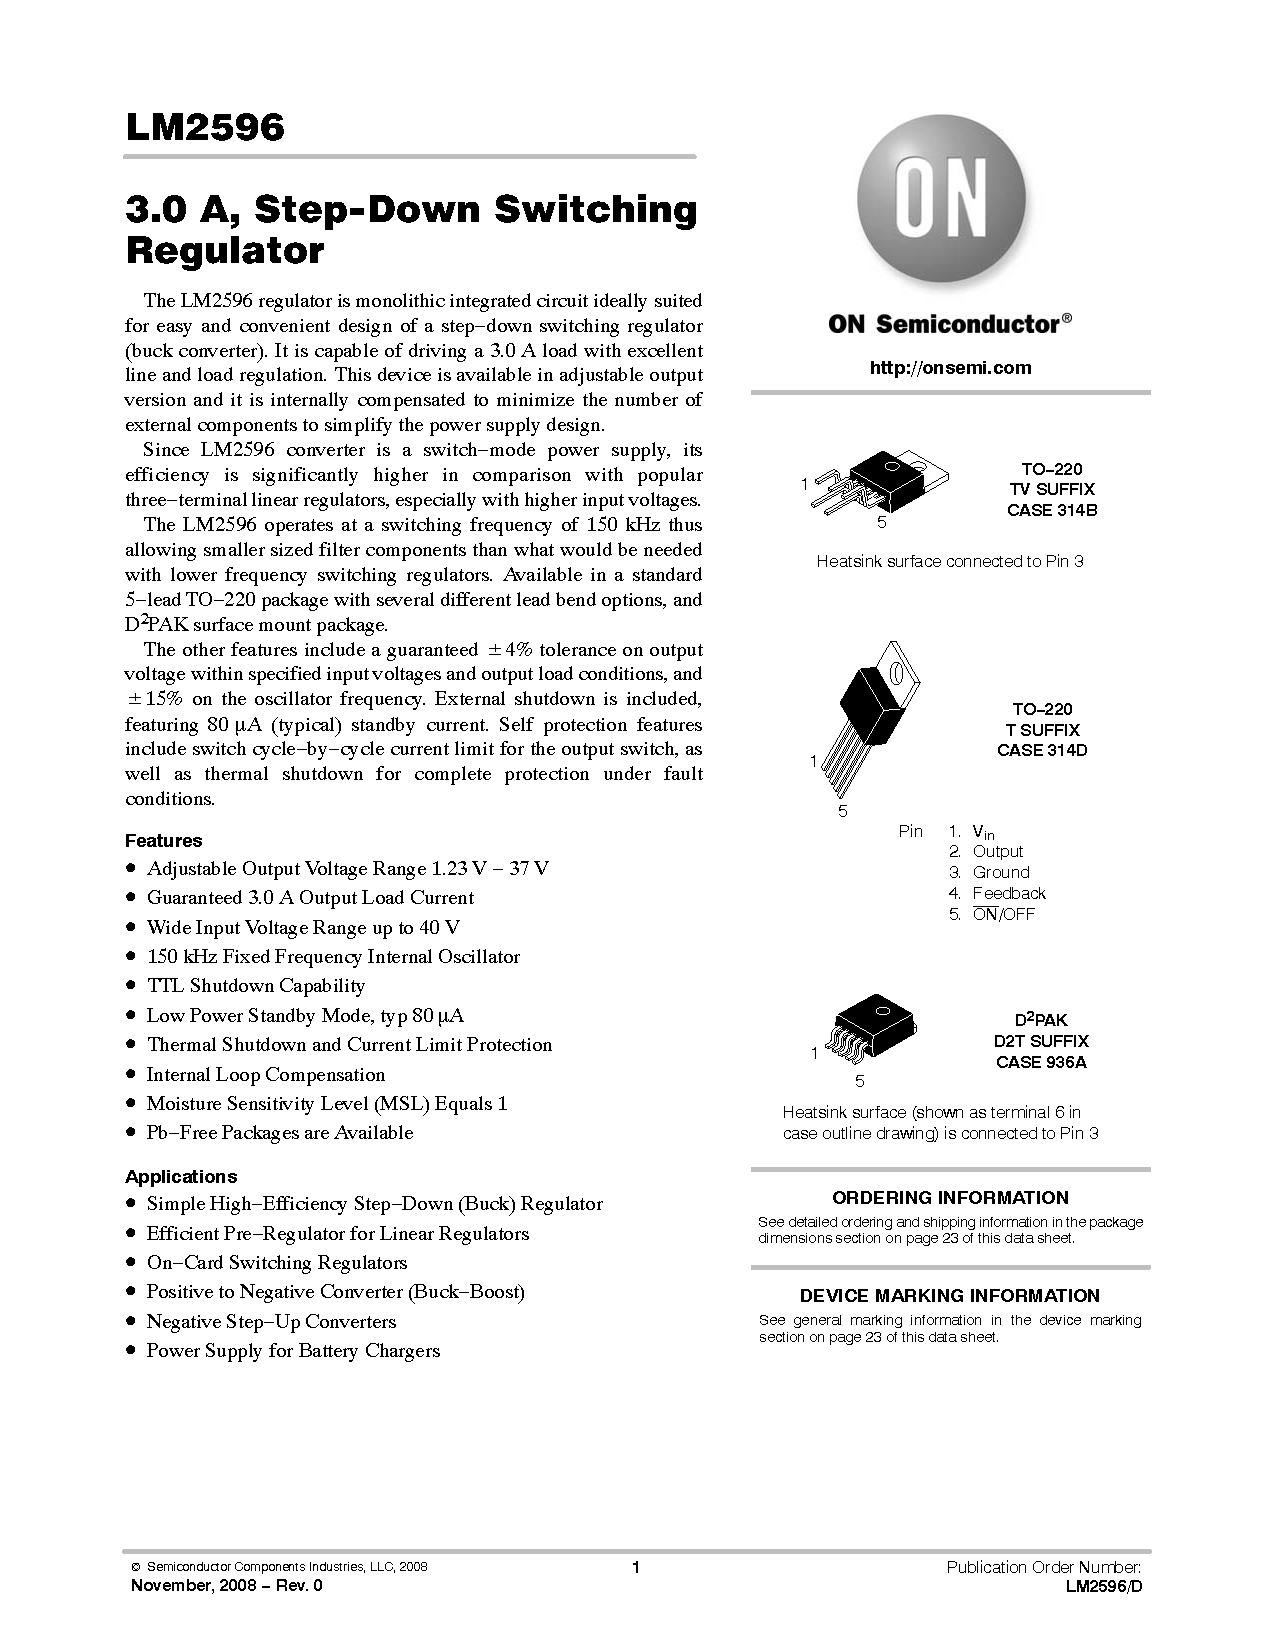
\includegraphics[scale=0.75, angle=0,page=1]{graphics/LM2596.PDF}
		\caption{Datenblatt LM2596-Seite 1}
		\label{datasheet:LM2596-1}
\end{figure}

\begin{figure}[H]
  \centering
		\includegraphics[scale=0.75, angle=0,page=7]{graphics/LM2596.PDF}
		\caption{Datenblatt LM2596-Seite 7 (Berechnung)}
		\label{datasheet:LM2596-2}
\end{figure}

\begin{figure}[H]
  \centering
		
\includegraphics[scale=0.8, angle=0,page=1]{graphics/LT1370.pdf}
		\caption{Datenblatt LT1370-Seite 1}
		\label{datasheet:LT1370-1}
\end{figure}

\begin{figure}[H]
  \centering
		
\includegraphics[scale=0.8, angle=0,page=7]{graphics/LT1370.pdf}
		\caption{Datenblatt LT1370-Seite 7 (Berechnung)}
		\label{datasheet:LT1370-2}
\end{figure}

\begin{figure}[H]
  \centering
		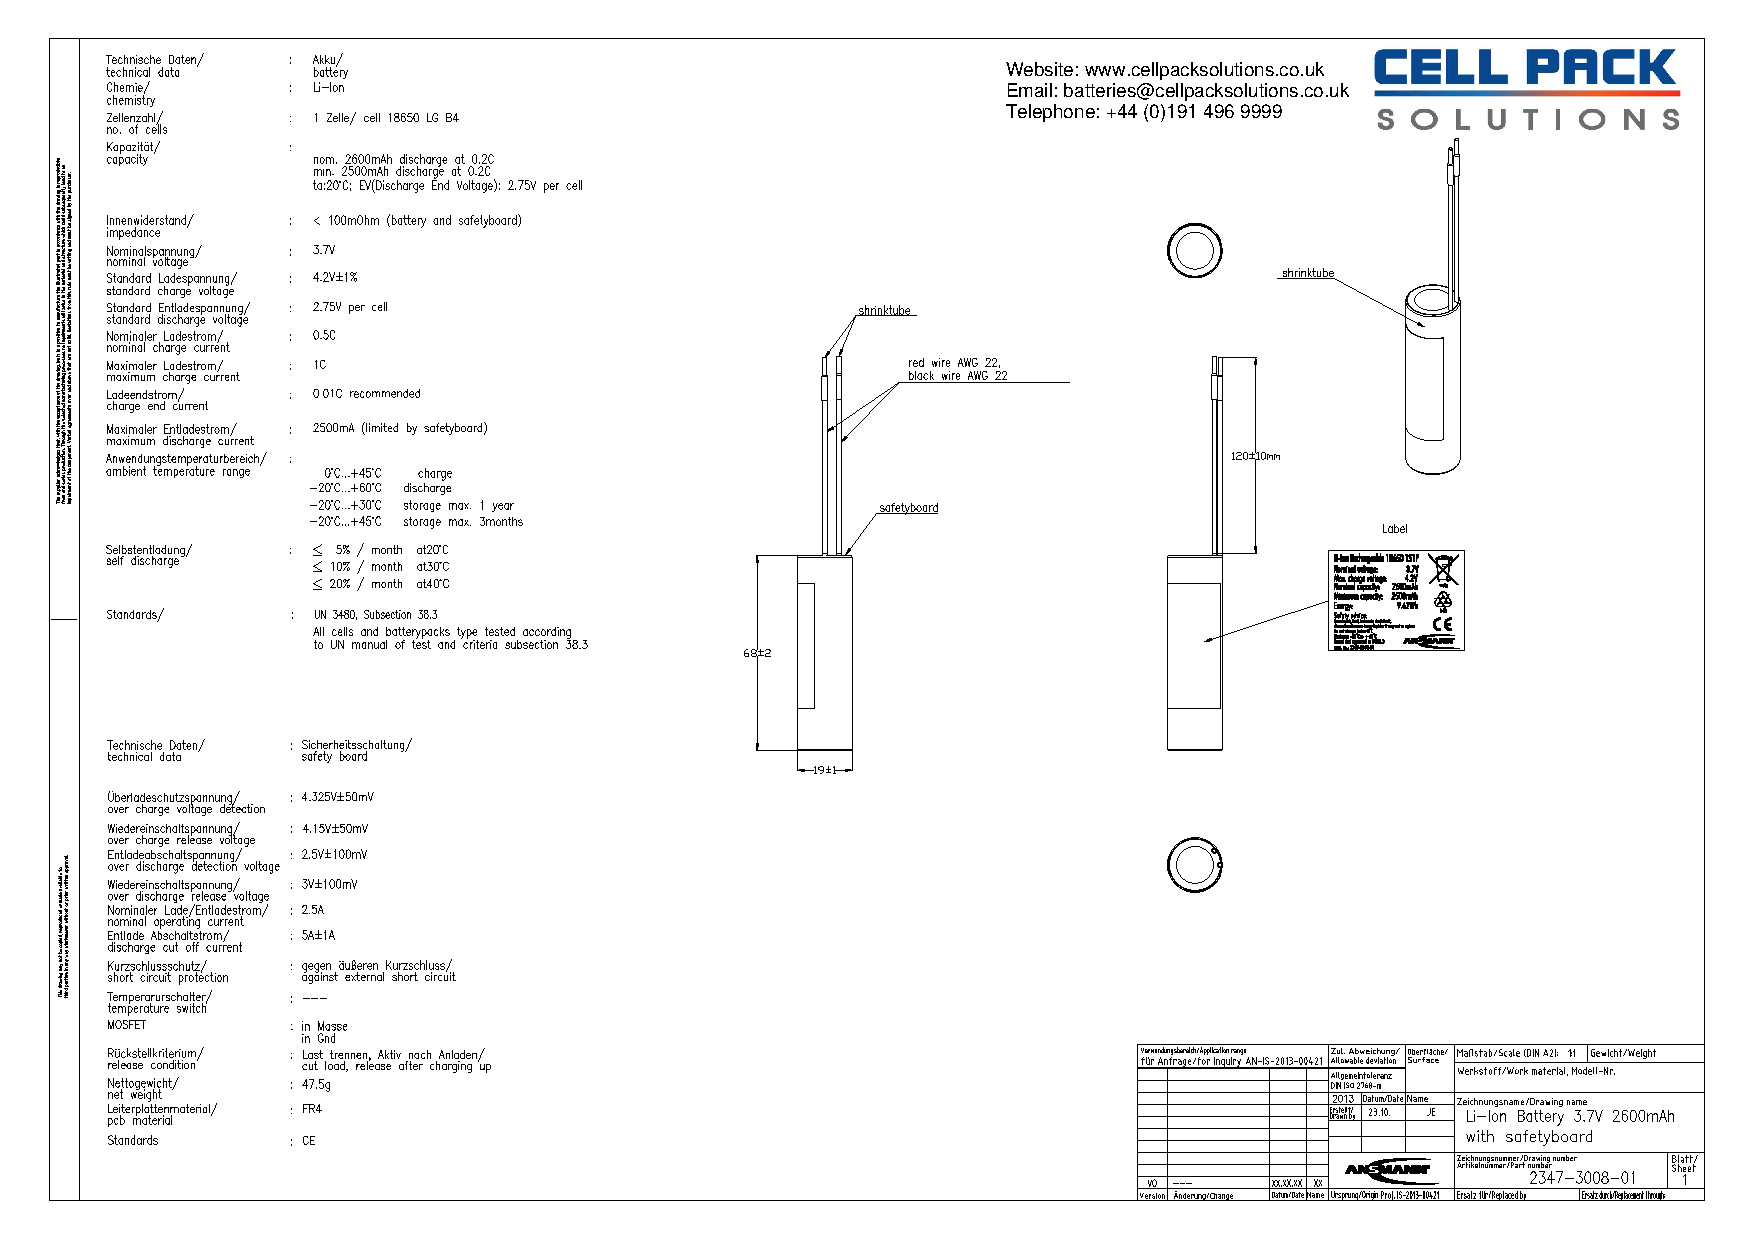
\includegraphics[scale=0.8, angle=90]{graphics/akku.pdf}
		\caption{Datenblatt Akku für Akkusteuerung}
		\label{datasheet:akku}
\end{figure}




\cmnt{

%==================================================================================
\clearpage\vfill\newpage
%==================================================================================
	% -???
	%iXH weiss nit, wieso da eine Leeseite zu sein hat.
	\vfill
	{\color{white} NIX}

}


%==================================================================================
\clearpage\vfill\newpage
%==================================================================================
\renewcommand\thesection{VII}
\section{\sc Zusammenfassung}

\subsection{Alexander Beiser}

Alexander Beiser war für einen Großteil der Spiellogik zuständig. Somit fallen darunter unter anderem:
\begin{itemize}
	\item{Logik des Ziehens der Spielfiguren,}
	\item{Schachmatt und Schach Abfrage,}
	\item{Speichern und Laden,}
	\item{und der Entwicklung des Computers (künstliche Intelligenz).}
\end{itemize}
Außerhalb des JavaChess Bereiches hat er, trotz Hindernissen, das Spiel auf den RaspberryPI portiert. Dazu hat er ein Gehäuse entwickelt und das Ganze mit einem Akku abgerundet, wodurch ein mobiles Spielen mit dem sogenannten ,,ChessPI'' möglich ist. \\
Dies ist das abgelieferte Ergebnis. Zusätzliche Aufgabe war es, eine Akkusteuerung selber zu entwerfen. Technisch gesehen sind zwei fertige Entwürfe dieser Akkusteuerung entwickelt worden, in der Messung der jeweiligen Schaltung stellte sich heraus, dass jedoch ein Laden mit diesen Schaltungen sehr lange dauern würde. Dadurch verfehlten diese Schaltungen ihren eigentlichen praktischen Nutzen. Die Weiterentwicklung dieser Schaltung, um dadurch ein Laden in entsprechender Zeit zu ermöglichen, schlugen fehl und somit wurde aus Zeitmangel heraus eine Powerbank verwendet.

\newpage
\subsection{Marcel Huber}

	Marcel Huber war für große Teile des ,,Frontends'' zuständig. Er entwickelte die grafische Benutzeroberfläche und gestaltete diese in Rücksprache mit den Testern so, dass sie ein optimales Spielerlebnis bietet. \\[2ex]
Er implementierte weitere Optionen und sorgte für eine passende Untermalung des Spielerlebnisses mithilfe von Soundeffekten.\\
Zudem wurde ein Spielmodus entwickelt, der es ermöglicht, zwei Spieler über ein Netzwerk spielen zu lassen. \\
Die Entwicklung der Android - Version wurde aufgrund von massivem Zeitmangel in der Frühphase eingestellt. 

\newpage
 \subsection{-Schlussfolgerung / Projekterfahrung}
 
 Das Projekt ist trotz einiger Rückschläge in weiten Teilen erfolgreich. Die künstliche Intelligenz ist stark genug um menschliche Spieler zu schlagen und das Spielen im Online Modus funktioniert tadellos. \\
	Beide Kandidaten hatten in einigen Punkten mit massiven Problemen zu kämpfen. Vor allem drei Punkte stellten sich als einen größeren Zeitaufwand heraus, als geplant:
\begin{enumerate}
	\item{Implementierung von JavaFX}
	\item{Das Portieren auf den RaspberryPI}
	\item{Die Entwicklung der Akkusteuerungsschaltung}
\end{enumerate}
1) - Das Verwenden von JavaFx bereitete anfänglich Probleme. Besonderns im Bereich des Multithreading, also das Auslagern von gewissen Aufgaben auf andere Abarbeitungsstränge sorgte im Zusammenhang mit JavaFx für Schwierigkeiten. Auch die mangelnde Ausbildung bezüglich JavaFx im Unterricht und die daraus folgende selbstständige Einarbeitung stellten eine besondere Herausforderung dar.  \\[1ex]
2) - Das Portieren auf den RaspberryPI stellte sich als einen sehr viel größeren Zeitaufwand heraus, als geplant. Oracle, also die Entwickler von Java, haben die Unterstützung von JavaFX für ,,Embedded-Processors'' eingestellt. Dadurch musste eine funktionierende Alternative gefunden werden. Nachdem diese Alternative gefunden wurde, stellte sich heraus, dass der Bildschirm in Verbindung mit Java einen gewissen ,,Offset'' besitzt, also der gedrückte Punkt stimmt nicht mit dem angezeigten überein. Dieser Fehler konnte ebenfalls unter entsprechendem Zeitaufwand behoben werden. \\[1ex]
3) - Die Entwicklung der Akkusteuerung stellte sich als ebenfalls größeres Problem als gedacht dar, da der Ladestrom viel zu klein war, um eine praktische Verwendung zu ermöglichen. \\[2ex]
Die wichtigste Projekterfahrung ist jedenfalls, dass bevor ein Projekt begonnen wird, eine Machbarkeitsstudie durchgeführt werden sollte. Dadurch können potentielle ,,Zeit fressende Singularitäten'' vermieden werden. Weiteres sollte man mehr Zeit für eventuelle Fehler einplanen, da der Zeitplan sonst unmöglich einzuhalten ist. \\
In zukünftigen Arbeiten im Team sollte man sich mehr absprechen und ständig in Kontakt über den momentanen Stand der Teammitglieder informiert sein, um die Effizienz und Effektivität zu steigern.

 \subsection{-Kostenaufstellung und Arbeitsnachweis} 
 \subsubsection{Kostenaufstellung}
 Hier erfolgt die Aufstellung der Projektkosten. Die Aufstellung erfolgt ohne Miteinberechnung der Versandkosten. \\
  
	\begin{center}
	
	
		\begin{tabular}{|c|c|c|}
		\hline
		 \sc Was & \sc Wie viel &  \sc Preis($\euro$)\\
		\specialrule{2.5pt}{1pt}{1pt}
		N-Mosfet			&		7							&		3.78				\\
		\hline
		4 Ohm Widerstand	&	5 (Packung)				&		1.51				\\
		\hline
		1N5408	 			& 10 (Packung)			&		5.2		\\
		\hline
		PNP-Transistor	&	10 (Packung)			&		2.99	\\
		\hline
		R-680 $\Omega$&	10 (Packung)			&		0.26		\\
		\hline
		R-3.9k$\Omega$	& 10 (Packung)			& 0.45		\\
		\hline
		1N5821				& 50 (Packung)			&	15.25		\\
		\hline
		Akku					&	2								& 35.94				\\
			\hline
		LM348					&		10 (Packung)		& 3.34				\\
			\hline
		R-1.8 k$\Omega$& 10 (Packung)			& 0.08				\\
			\hline
		LM2596				&	1								&	3.87			\\
			\hline
		C-100$\mu$F		&	5 (Packung)				&	1.23			\\
			\hline
		L-33 $\mu$H		&	1								& 2.89				\\
			\hline
		C-220$\mu$F		&	5 (Packung)				&	0.59			\\
			\hline
		Sicherung 4A		&	10 (Packung)			&	0.73			\\
			\hline
		Raspberry 3		&	1								&	61.41			\\
			\hline
		7'' Touchscreen	&	1								&	57.7			\\
			\hline
		Micro-USB Buchse& 1									&	 20.99			\\
			\hline
		Schalter				&	1								&			12.99	\\
			\hline
		M-3-Stange			&		1							& 0.89				\\
			\hline
			USB-2.0 Kabel		&	1								&	9.99			\\
			\hline
			Mikro-USB-Verlängerung		&	1								&		9.99		\\
			\hline
			LT-1370-SMD		&	1								&		11.41		\\
			\hline
			LT-1370-TO220		&	1								&		21.99		\\
			\hline
			Powerbank-RP-PB17		&	1								&		17.99		\\
			\specialrule{2.5pt}{1pt}{1pt}
			\multicolumn{2}{|c|}{$\sum$} & 316.31\\
			\hline
	\end{tabular}
\end{center}


  \subsubsection{Arbeitsnachweis Diplomarbeit}
	\label{SUBSEC:WORKDONE}	
	\cmnt{
	02.10.2017 -Alexander Beiser: Schachmatt Algorithmus und Vervollständigung des Hot-Seat Modus -Marcel Huber: Implementierung der Netzwerkfähigkeit

06.11.2017 -Alexander Beiser: Entwicklung der künstlichen Intelligenz -Marcel Huber: Implementierung von Java FX.

18.12.2017 -Alexander Beiser: Raspberry-PI Implementierung und Design des Gehäuses -Marcel Huber: Komplettüberarbeitung der GUI für eine bessere Benutzer-Erfahrung

04.02.2018 -Alexander Beiser: Entwicklung der Akku-Steuerungsschaltung und Einbau dieser -Marcel Huber: Portierung auf Android

05.03.2018 -Alexander Beiser: Durchführung einer Beta-Phase und Fehlerbehebungen -Marcel Huber: Durchführung einer Beta-Phase und Fehlerbehebungen 
		
	}
	
% Please add the following required packages to your document preamble:
% \usepackage[normalem]{ulem}
% \useunder{\uline}{\ul}{}
\begin{table}[H]
\centering
\begin{tabular}{ccccc}
\multicolumn{5}{c}{\textbf{Arbeitsaufstellung}}                                                                                                                                                                                                                                  \\ \hline
\multicolumn{1}{|c|}{{\ul Was  }}                                                                                                     & \multicolumn{1}{c|}{{\ul Person}} & \multicolumn{1}{c|}{{\ul Stunden}} & \multicolumn{1}{c|}{{\ul Von}}  & \multicolumn{1}{c|}{{\ul Bis}}  \\ \hline
\multicolumn{5}{|c|}{\textit{Beginn der Diplomarbeit - 14.09.2017}}                                                                                                                                                                                                              \\ \hline
\multicolumn{1}{|c|}{\begin{tabular}[c]{@{}c@{}}Schachmatt Algorithmus\\ und Hotseat Modus\end{tabular}}                            & \multicolumn{1}{c|}{Beiser}       & \multicolumn{1}{c|}{30}            & \multicolumn{1}{c|}{14.09.2017} & \multicolumn{1}{c|}{02.10.2017} \\ \hline
\multicolumn{1}{|c|}{\begin{tabular}[c]{@{}c@{}}Implementierung der \\ Netzwerkfähigkeit\end{tabular}}                              & \multicolumn{1}{c|}{Huber}        & \multicolumn{1}{c|}{30}            & \multicolumn{1}{c|}{14.09.2017} & \multicolumn{1}{c|}{02.10.2017} \\ \hline
\multicolumn{5}{|c|}{{\textit{Meilenstein 1 - 02.10.2017}}}                                                                                                                                                                                                                           \\ \hline
\multicolumn{1}{|c|}{\begin{tabular}[c]{@{}c@{}}Entwicklung der künstlichen\\ Intelligenz\end{tabular}}                             & \multicolumn{1}{c|}{Beiser}       & \multicolumn{1}{c|}{30}            & \multicolumn{1}{c|}{02.10.2017} & \multicolumn{1}{c|}{06.11.2017} \\ \hline
\multicolumn{1}{|c|}{Implementierung von JavaFX}                                                                                    & \multicolumn{1}{c|}{Huber}        & \multicolumn{1}{c|}{40}            & \multicolumn{1}{c|}{02.10.2017} & \multicolumn{1}{c|}{06.11.2017} \\ \hline
\multicolumn{5}{|c|}{{\textit{Meilenstein 2 - 06.11.2017}}}                                                                                                                                                                                                                           \\ \hline
\multicolumn{1}{|c|}{\begin{tabular}[c]{@{}c@{}}Raspberry-PI Implementierung\\ und Design des Gehäuses\end{tabular}}                & \multicolumn{1}{c|}{Beiser}       & \multicolumn{1}{c|}{35}            & \multicolumn{1}{c|}{06.11.2017} & \multicolumn{1}{c|}{18.12.2017} \\ \hline
\multicolumn{1}{|c|}{\begin{tabular}[c]{@{}c@{}}Komplettüberarbeitung der GUI\\ für eine bessere Benutzer\\ Erfahrung\end{tabular}} & \multicolumn{1}{c|}{Huber}        & \multicolumn{1}{c|}{34}            & \multicolumn{1}{c|}{06.11.2017} & \multicolumn{1}{c|}{18.12.2017} \\ \hline
\multicolumn{5}{|c|}{{\textit{Meilenstein 3 - 18.12.2017}}}                                                                                                                                                                                                                           \\ \hline
\multicolumn{1}{|c|}{\begin{tabular}[c]{@{}c@{}}Entwicklung der Akku-\\ Steuerschaltung und Einbau \\ dieser\end{tabular}}          & \multicolumn{1}{c|}{Beiser}       & \multicolumn{1}{c|}{34}            & \multicolumn{1}{c|}{18.12.2017} & \multicolumn{1}{c|}{04.02.2018} \\ \hline
\multicolumn{1}{|c|}{Portierung auf Android}                                                                                        & \multicolumn{1}{c|}{Huber}        & \multicolumn{1}{c|}{15}            & \multicolumn{1}{c|}{18.12.2017} & \multicolumn{1}{c|}{04.02.2018} \\ \hline
\multicolumn{5}{|c|}{{\textit{Meilenstein 4 - 04.02.2018}}}                                                                                                                                                                                                                           \\ \hline
\multicolumn{1}{|c|}{\begin{tabular}[c]{@{}c@{}}Durchführung einer Beta-Phase\\ und Fehlerbehebungen\end{tabular}}                  & \multicolumn{1}{c|}{Beiser}       & \multicolumn{1}{c|}{30}            & \multicolumn{1}{c|}{04.02.2018} & \multicolumn{1}{c|}{05.03.2018} \\ \hline
\multicolumn{1}{|c|}{\begin{tabular}[c]{@{}c@{}}Durchführung einer Beta-Phase und \\ Fehlerbehebungen\end{tabular}}                  & \multicolumn{1}{c|}{Huber}        & \multicolumn{1}{c|}{42}            & \multicolumn{1}{c|}{04.02.2018} & \multicolumn{1}{c|}{05.03.2018} \\ \hline
\multicolumn{5}{|c|}{{\textit{Meilenstein Dokumentation}}} \\ \hline
\multicolumn{1}{|c|}{\begin{tabular}[c]{@{}c@{}}Dokumentation\end{tabular}}                  & \multicolumn{1}{c|}{Beiser}       & \multicolumn{1}{c|}{21}            & \multicolumn{1}{c|}{14.09.2017} & \multicolumn{1}{c|}{04.04.2018} \\ \hline
\multicolumn{1}{|c|}{\begin{tabular}[c]{@{}c@{}}Dokumentation\end{tabular}}                  & \multicolumn{1}{c|}{Huber}        & \multicolumn{1}{c|}{19}            & \multicolumn{1}{c|}{14.09.2017} & \multicolumn{1}{c|}{04.04.2018} 
                                                                                                                                                                                                                           \\ \hline
\end{tabular}
\caption{Arbeitsaufstellung nach Meilensteinen}
\label{table:workgeneral}
\end{table}

\label{LastPage}
%\addtocontents{toc}{\protect\end{multicols}}
\end{document}





%XH 25Feb17:Anpassung gem.YH-neueVorlage 'YH-RbN1-moodle2-Vorlage_DA_sRDP_19102016.docx'
%	RbP:Logo Dicke scalable
%	RbN:Logo
%bis 21Mar17: Warten auf Modifikation Greif-Mikaelyan-Widmann (nicht erhalten)
%XH 21Mar17: Finalisierung (ohne Greif-Mikaelyan-Widmann)
%XH:RdC-1547-2213	Tests variablem '\{0.12}' in 'fancyheader'-Kopfzeilen: vergeblich
%XH:RdD:0857-1112	Text-Check2
%XH:RdF:0914-1737	Preambel-Header kommentieren+ausmisten, Abgleich m. YH'docx'-Version
